\documentclass[11pt]{article}

\usepackage{amsmath}
\usepackage{mathtools}
\usepackage{amssymb}
\usepackage{wrapfig}
\usepackage{fancyhdr}
\usepackage{tikz-qtree}
\usepackage{tikz-qtree-compat}
\usepackage[normalem]{ulem}
\usepackage{tikz}
\usepackage{graphicx}
\usepackage{lineno}
\usepackage{floatrow}
\usepackage{bm}
\usepackage{cite}

\DeclareMathOperator*{\argmin}{argmin}
\DeclareMathOperator*{\argmax}{argmax}

\oddsidemargin0cm
\topmargin-2cm
\textwidth16.5cm
\textheight23.5cm 

\newcommand{\question}[2] {\vspace{.25in} \hrule\vspace{0.5em}
\noindent{\bf #1: #2} \vspace{0.5em}
\hrule \vspace{.10in}}
\renewcommand{\part}[1] {\vspace{.10in} {\bf (#1)}}
\linespread{1.5}

\setlength{\parindent}{0pt}
\setlength{\parskip}{5pt plus 1pt}
 
\DeclarePairedDelimiter\abs{\lvert}{\rvert}%


\begin{document}
\medskip        

\thispagestyle{plain}
{\Large Interrogating theoretical models of neural computation with deep inference} \\
Sean R. Bittner$^{1}$, Agostina Palmigiano$^{1}$, Alex T. Piet$^{2,3,4}$, Chunyu A. Duan$^{5}$, Carlos D. Brody$^{2,3,6}$, \\
Kenneth D. Miller$^{1}$, and John P. Cunningham$^{7}$.

{\small
$^{1}$Department of Neuroscience, Columbia University, \\
$^{2}$Princeton Neuroscience Institute, \\
$^{3}$Princeton University, \\
$^{4}$Allen Institute for Brain Science, \\
$^{5}$Institute of Neuroscience, Chinese Academy of Sciences, \\
$^{6}$Howard Hughes Medical Institute, \\
$^{7}$Department of Statistics, Columbia University
}

\linenumbers
\section{Abstract}
%When analytic derivation of the relationship between model parameters and computational properties is intractable, approximate inference and simulation-based techniques are relied upon for scientific insight.
%We bring the use of deep generative models for probabilistic inference to bear on this problem, learning complex distributions of parameters that produce the specified properties of computation.
A cornerstone of theoretical neuroscience is the circuit model: a system of equations that captures a hypothesized neural mechanism.  
Such models are valuable when they give rise to an experimentally observed phenomenon -- whether behavioral or a pattern of neural activity -- and thus can offer insights into neural computation.
The operation of these mechanistic circuits, like all models, critically depends on the choices of model parameters.
A key process in circuit modeling is then to identify the model parameters consistent with observed phenomena: to solve the inverse problem.
To solve challenging inverse problems modeling neural datasets, neuroscientists have used statistical inference techniques to much success. 
However, most research in theoretical neuroscience focuses on how computation emerges in biologically interpretable circuit models, and how the model parameters govern computation; it is not focused on the latent structure of empirical models of noisy experimental datasets.
In this work, we present a novel technique that brings the power and versatility of the probabilistic modeling toolkit to theoretical inverse problems.
Our method uses deep neural networks to learn parameter distributions with rich structure that have specific computational properties in biologically relevant models.
This methodology is explained through a motivational example inferring conductance parameters in an STG subcircuit model.
Then, with RNNs of increasing size, we show that only EPI allows precise control over the behavior of inferred parameters, and that EPI scales better in parameter dimension than alternative techniques.
In the remainder of this work, we explain novel theoretical insights through the examination of intricate parametric structure in complex circuit models.
In a model of primary visual cortex with multiple neuron-types, where analysis becomes untenable with each additional neuron-type, we discovered how noise distributed across neuron-types governs the excitatory population.
Finally, in a model of superior colliculus, we identified and characterized two distinct regimes of connectivity that facilitate switching between opposite tasks amidst interleaved trials. 
We also found that all task-switching connectivities in this model reproduce behaviors from inactivation experiments, further establishing this hypothesized circuit model.
Beyond its scientific contribution, this work illustrates the variety of analyses possible once deep learning is harnessed towards solving theoretical inverse problems.


%-------- old sentences -----------

%Historically, the gold standard has been to analytically derive the relationship between model parameters and computational properties.  
%However, this enterprise quickly becomes infeasible as biologically realistic constraints are included into the model increasing its complexity, often resulting in \emph{ad hoc} approaches to understanding the relationship between model and computation.
%Importantly, the techniques we introduce offer a principled means to understand the implications of model parameter choices on computational properties of interest.  
%We then use it to go beyond linear theory of neuron-type input-responsivity in a model of primary visual cortex, gain a mechanistic understanding of rapid task switching in superior colliculus models, and attribute error to connectivity properties in recurrent neural networks solving a simple mathematical task.
%More generally, this work suggests a departure from realism vs tractability considerations, towards the use of modern machine learning for sophisticated interrogation of biologically relevant models.
%%%%%%%%%%%%%%%%%%%%%%%%%%%%%%%%%%%
%%%%%%%%%%%%%%%%%%%%%%%%%%%%%%%%%%%

\section{Introduction}
The fundamental practice of theoretical neuroscience is to use a mathematical model to understand neural computation, whether that computation enables perception, action, or some intermediate processing.  
A neural circuit is systematized with a set of equations -- the mechanistic model -- and these equations are motivated by biophysics, neurophysiology, and other conceptual considerations \cite{kopell1988coupled,  marder1998biophysics, abbott2008theoretical, wang2010neurophysiological}.
The function of this system is governed by the choice of model \emph{parameters}, which when configured in a particular way, give rise to a measurable signature of a computation.   
The work of analyzing a model then requires solving the inverse problem: given a computation of interest, how can we reason about particular parameter configurations?  
The inverse problem is crucial for reasoning about likely parameter values, uniquenesses and degeneracies, and predictions made by the model \cite{gutenkunst2007universally, o2014cell}.

Consider the idealized practice: one carefully designs a model and analytically derives how computational properties determine model parameters.
Seminal examples of this gold standard include our field's understanding of memory capacity in associative neural networks \cite{hopfield1982neural}, chaos and autocorrelation timescales in random neural networks \cite{sompolinsky1988chaos}, the paradoxical effect \cite{tsodyks1997paradoxical}, and decision making \cite{wong2006recurrent}.
Unfortunately, as circuit models include more biological realism, theory via analytical derivation becomes intractable.
Still, we can gain insight into these complex models by identifying the distribution of parameters that produce computations.
By solving the inverse problem in this way, scientific analysis of biologically realistic models is made possible \cite{foster1993significance, prinz2004similar, achard2006complex, o2014cell, alonso2019visualization}.

While theoretical neuroscience is concerned with how model parameters govern  computational properties, existing methodology for statistical inference in neuroscience \cite{kass2001spike, brown1998statistical, paninski2004maximum, truccolo2005point, schneidman2006weak, druckmann2007novel, turner2007maximum, byron2009gaussian, macke2011empirical, park2011bayesian, granot2013stimulus, latimer2015single, lakshminarasimhan2018dynamic, duncker2019learning, ladenbauer2019inferring, gao2016linear, zhao2017recursive, barello2018sparse, pandarinath2018inferring, wiltschko2015mapping, johnson2016composing, batty2019behavenet} (see review, \cite{paninski2018neural}) requires that parameters be conditioned on an explicit dataset.
The scientific insight for a model of computation is then limited by the quantity and quality of available neural data.
Even with a vast amount of high-quality recordings, neural data often reflect uninstructed behaviors \cite{niell2010modulation, saleem2013integration, musall2019single}, and thus may only reflect the computation of interest amidst a sea of task-irrelevant factors. 
A common alternative is to synthesize an explicit dataset that is exemplary of that computation, so that the framework of statistical inference can be applied for parameter identification.
In this case, well-defined computational properties are being shoehorned into artificial datasets for the purpose of methodological compatibility.

Another key challenge is that as models of computation become more complex, statistical inference becomes intractable.
Such mechanistic models in theoretical neuroscience are noisy systems of differential equations that can only be sampled or realized through forward simulation \cite{dayan2003theoretical, izhikevich2007dynamical}; they lack a tractable likelihood function, which is necessary for statistical inference.
Therefore, the most popular approaches to parameter inference in mechanistic models have been simulation-based inference methods \cite{sisson2007sequential, liepe2014framework}, in which reasonable parameters are obtained via simulation and rejection.
A new class of techniques \cite{gonccalves2019training, papamakarios2019sequential, hermans2020likelihood} use deep learning to improve upon traditional simulation-based inference approaches.
However, to use these methods in theoretical neuroscience, we must represent computation with an explicit dataset in some way.
Theorists are therefore barred from using the probabilistic modeling toolkit for science with circuit models, unless they reformulate their inverse problem into a framework for observational datasets.

%
%Existing approaches to the inverse problem in theoretical neuroscience fall short in three key ways. 
%First, theoretical models of neural computation aim to reflect a complex biological reality, and as a result, such models lack tractable likelihoods.
%Without an efficient calculation of the probability of model properties given model parameters, neuroscientists resort to approximate Bayesian computation \cite{beaumont2002approximate, marjoram2003markov, sisson2007sequential}, which requires a rejection heuristic, scales poorly, and only produces sets of accepted parameters lacking probabilities.
%Second, there is an undesirable trade-off between the flexibility and sampling speed of approximated posterior distributions.
%Sampling-based inference approaches (e.g. ABC and Markov chain Monte Carlo (MCMC) \cite{hastings1970monte, metropolis1953equation}) confer flexible approximations, yet scale poorly in number of parameters.
%While variational inference (VI) \cite{saul1998mean} often results in fast posterior sampling, existing practice relies heavily on simplified classes of distributions \cite{rezende2015variational}.  
%Third, such parameter inference methods are designed to operate on experimentally collected data-sets.
%Ultimately, the objects of interest in theoretical neuroscience are phenomena or features of the model rather than singular data-sets.

%To address these three challenges, we developed an inference methodology -- `emergent property inference' -- which learns a distribution over parameter configurations in a theoretical model.  
%This distribution has two critical properties: \emph{(i)} it is chosen such that draws from the distribution (parameter configurations) correspond to systems of equations that give rise to a specified emergent property (a set of constraints); and \emph{(ii)} it is chosen to have maximum entropy given those constraints, such that we identify all likely parameters and can use the distribution to reason about parametric sensitivity and degeneracies \cite{transtrum2015perspective}.  
%First, we use stochastic gradient techniques in the spirit of likelihood-free variational inference \cite{tran2017hierarchical} to enable inference in likelihood-free models of neural computation.
%Second, we stipulate a bijective deep neural network that induces a flexible family of probability distributions over model parameterizations with a probability density we can calculate \cite{rezende2015variational, dinh2017density, papamakarios2017masked}, which confers fast sampling and sensitivity measurements.
%Third, we quantify the notion of emergent properties as a set of moment constraints on datasets generated by the model.  
%Thus, an emergent property is not a single data realization, but a phenomenon or a feature of the model.
%Conditioning on an emergent property requires a variant of deep probabilistic inference methods, which we have previously introduced \cite{loaiza2017maximum}.
%Taken together, emergent property inference (EPI) provides a methodology for inferring parameter configurations consistent with a particular emergent phenomena in theoretical models.
%We use a classic example of parametric degeneracy in a biological system, the stomatogastric ganglion \cite{goldman2001global}, to motivate and clarify the technical details of EPI.
%
%These challenges motivate the development of a novel inference framework called emergent property inference (EPI).
%As an adaption of variational inference \cite{saul1998mean}, EPI infers parameter distributions that produce an emergent property: not a singular dataset, but a collection of datasets exhibiting some mathematical criteria.
%EPI constrains the predictions of the inferred parameter distribution to produce the emergent property, which requires a variant of probabilistic inference methods \cite{loaiza2017maximum}.
%Importantly, EPI uses deep learning to make rich, flexible approximations to the parameter distribution \cite{rezende2015variational} that produces an emergent property.
%The structure captured by these deep probability distributions are scientifically valuable, revealing the sensitivity and robustness of the emergent property to different parameter combinations.
%Perhaps most powerfully, EPI facilitates inference in mechanistic models, allowing theorists to capture rich parametric structure in biologically realistic models that is conditioned upon the emergent phenomena of interest.

To address the methodological incongruity between explicit datasets and emergent properties, we present a statistical inference method for conditioning parameters of neural circuit models directly on computation.
In this work, we define computation by an emergent property, which is a statistical description of the phenomena to be produced by the neural circuit model.
In emergent property inference (EPI), we infer the distribution of model parameters that produce this emergent property.
With EPI, parameters are conditioned directly on an implicit dataset defined by the computation of interest.
By using recent optimization techniques \cite{loaiza2017maximum}, EPI uses deep learning to make rich, flexible approximations to the parameter distributions \cite{rezende2015variational}, the structure of which reveals scientific insight about how parameters govern the emergent property.


Equipped with this method, we prove out the potential of EPI by demonstrating its capabilities and presenting novel theoretical findings borne from its analysis.
First, we show EPI's ability to handle mechanistic models using a classic model of parametric degeneracy in biology: the stomatogastric ganglion \cite{goldman2001global, gutierrez2013multiple}.
Then, we show EPI's scalability to high dimensional parameter distributions by inferring connectivities of recurrent neural networks (RNNs) that exhibit stable, yet amplified responses -- a hallmark of neural responses throughout the brain \cite{murphy2009balanced, hennequin2014optimal, bondanelli2019population}.
In a model of primary visual cortex (V1) \cite{litwin2016inhibitory, palmigiano2020structure} with different neuron-types, we show that the equation for excitatory variability become analytically intractable as more populations are added.
Strikingly, the way in which noisy inputs across neuron-types governs excitatory variability is salient in the visualized structure of the EPI inferred parameter distribution.
Finally, we investigated the possible connectivities of superior colliculus (SC) that allow execution of different tasks on intervleaved trials \cite{duan2018collicular}.
EPI discovered a rich distribution containing two connectivity regimes with different solution classes.
We queried the deep probability distribution learned by EPI to produce a mechanistic understanding of cortical responses in each regime. 
Intriguingly, all inferred connectivities reproduced results from optogenetic inactivation experiments in this behavioral paradigm -- emergent phenomena that EPI was not conditioned upon.
These theoretical insights afforded by EPI illustrate the value of deep inference for the interrogation of neural circuit models.

%-------- old sentences -----------

%The inverse problem is crucial for reasoning about likely parameter values, uniquenesses and degeneracies, attractor states and phase transitions, and predictions made by the model.

%This creates an unfavorable tradeoff.  On the one hand, one may tractably analyze systems of equations with unrealistic assumptions (for example symmetry or gaussianity), mathematically formalizing how parameters affect computation in a too-simple model.  
%On the other hand, one may choose a more biologically accurate, scientifically relevant model at the cost of \emph{ad hoc} approaches to analysis (such as simply examining simulated activity), potentially resulting in bad inference of parameters and thus erroneous scientific predictions or conclusions.

%Exact Bayesian inference is rarely tractable, so Markov chain Monte Carlo (MCMC) and variation inference (VI) techniques are used in practice.

% now transition to deep ML...
%Of course, this same tradeoff has been confronted in many scientific fields characterized by the need to do inference in complex models.
%In response, the machine learning community has made remarkable progress in recent years, via the use of deep neural networks as a powerful inference engine: a flexible function family that can map observed phenomena (in this case the measurable signal of some computation) back to probability distributions quantifying the likely parameter configurations. 
%One celebrated example of this approach from machine learning, of which we draw key inspiration for this work, is the variational autoencoder \cite{kingma2013auto, rezende2014stochastic}, which uses a deep neural network to induce an (approximate) posterior distribution on hidden variables in a latent variable model, given data. 

%However, these inference tools have not significantly influenced the study of theoretical neuroscience models, for at least three reasons.
%First, at a practical level, the nonlinearities and dynamics of many theoretical models are such that conventional inference tools typically produce a narrow set of insights into these models.
%Indeed, only in the last few years has deep learning research advanced to a point of relevance to this class of problem.
%Second, the object of interest from a theoretical model is not typically data itself, but rather a qualitative phenomenon -- inspection of model behavior, or better, a measurable signature of some computation -- an \emph{emergent property} of the model.  
%Third, because theoreticians work carefully to construct a model that has biological relevance, such a model as a result often does not fit cleanly into the framing of a statistical model.
%Technically, because many such models stipulate a noisy system of differential equations that can only be sampled or realized through forward simulation, they lack the explicit likelihood and priors central to the probabilistic modeling toolkit.

%First, we stipulate a bijective deep neural network that induces a flexible family of probability distributions over model parameterizations with a probability density we can calculate \cite{rezende2015variational, dinh2016density, papamakarios2017masked}.
%Second, we quantify the notion of emergent properties as a set of moment constraints on datasets generated by the model.  
%Thus, an emergent property is not a single data realization, but a phenomenon or a feature of the model, which is ultimately the object of interest in theoretical neuroscience.
%Conditioning on an emergent property requires a variant of deep probabilistic inference methods, which we have previously introduced \cite{loaiza2017maximum}.
%Third,  because we cannot assume the theoretical model has explicit likelihood on data or the emergent property of interest, we use stochastic gradient techniques in the spirit of likelihood free variational inference \cite{tran2017hierarchical}.    
%Taken together, emergent property inference (EPI) provides a methodology for inferring parameter configurations consistent with a particular emergent phenomena in theoretical models.
%We use a classic example of parametric degeneracy in a biological system, the stomatogastric ganglion \cite{goldman2001global}, to motivate and clarify the technical details of EPI.

%First, we use EPI to produce a set of verifiable hypotheses of input-responsivity in a four neuron-type dynamical model of primary visual cortex; we then validate these hypotheses in the model.
%Second, we demonstrated how the systematic application of EPI to levels of task performance can generate experimentally testable hypotheses regarding connectivity in superior colliculus.  
%Third, we use EPI to uncover the sources of error in a low-rank recurrent neural network executing a simple mathematical task.  

%%%%%%%%%%%%%%%%%%%%%%%%%%%%%%%%%%%
%%%%%%%%%%%%%%%%%%%%%%%%%%%%%%%%%%%

\section{Results}
\subsection{Motivating emergent property inference of theoretical models} \label{results_motivating}

%Consideration of the typical workflow of theoretical modeling clarifies the need for emergent property inference.  
Consideration of the typical workflow of theoretical modeling clarifies the need for emergent property inference.  
First, one designs or chooses an existing model that, it is hypothesized, captures the computation of interest. 
To ground this process in a well-known example, consider the stomatogastric ganglion (STG) of crustaceans, a small neural circuit which generates multiple rhythmic muscle activation patterns for digestion \cite{marder2002cellular}.
Despite full knowledge of STG connectivity and a precise characterization of its rhythmic pattern generation, biophysical models of the STG have complicated relationships between circuit parameters and computation \cite{goldman2001global, prinz2004similar}.
%A model of the STG \cite{gutierrez2013multiple} is shown schematically in Figure \ref{fig:STG}A, and note that the behavior of this model will be critically dependent on its parameterization -- the choices of conductance parameters $z = [g_{\text{el}}, g_{\text{synA}}]$.
A subcircuit model of the STG \cite{gutierrez2013multiple} is shown schematically in Figure \ref{fig:STG}A.
The jagged connections indicate electrical coupling having electrical conductance $g_{\text{el}}$, smooth connections in the diagram are inhibitory synaptic projections having strength $g_{\text{synA}}$ onto the hub neuron, and $g_{\text{synB}}=5$nS for mutual inhibitory connections.
Note that the behavior of this model will be critically dependent on its parameterization -- the choices of conductance parameters $\mathbf{z} = [g_{\text{el}}, g_{\text{synA}}]$.
Specifically, the two fast neurons ($f1$ and $f2$) mutually inhibit one another, and oscillate at a faster frequency than the mutually inhibiting slow neurons ($s1$ and $s2$).  
The hub neuron (hub) couples with either the fast or slow population, or both.  

Second, once the model is selected, one must specify what the model should produce.
In this STG model, we are concerned with neural spiking frequency, which emerges from the dynamics of the circuit model \ref{fig:STG}B.
An emergent property studied by Guttierez et al. of this stochastic model is the hub neuron firing at an intermediate frequency between the intrinsic spiking rates of the fast and slow populations.
This emergent property is shown in Figure \ref{fig:STG}C at an average frequency of 0.55Hz.
Our notion of intermediate hub frequency is not strictly 0.55Hz, but also moderate deviations of this frequency between the fast (.35Hz) and and slow (.68Hz) frequencies, which are quantified in the emergent property with variance {0.025$^2$Hz$^2$}.
%To continue our running STG example, one such emergent property is the phenomenon of \emph{network syncing} -- in certain parameter regimes, the frequency of the hub neuron matches that of the fast and slow populations at an intermediate frequency.


%Third, qualitative parameter analysis ensues: since precise mathematical analysis is intractable in this model, a brute force sweep of parameters is done \cite{gutierrez2013multiple}.
%Subsequently, a qualitative description is formulated to describe the different parameter configurations that lead to the emergent property.  
%In this last step lies the opportunity for a precise quantification of the emergent property as a statistical feature of the model. 
% Once we have such a methodology, we can infer a probability distribution over parameter configurations that produce this emergent property.
%Sensitivity analyses \cite{raue2009structural} are also used to identify which parameter contributions have the greatest effect.
%In this last step lies the opportunity for a precise quantification of the emergent property as a statistical feature of the model.
Third, the model parameters producing these outputs are inferred.
To infer the STG parameters of intermediate hub frequency with existing methodology, we  need an explicit dataset: experimentally recorded or synthesized.
By precisely quantifying the emergent property of interest as a statistical feature of the model, we use EPI to condition directly on this emergent property.
EPI learns a probability distribution of model parameters constrained to produce the emergent property.
In this last step lies the opportunity for a shift away from a dataset-oriented representation of model output towards that of an implicit dataset, where the only structure is the emergent property of interest.
%Most often, brute-force parameter sweeps or rejection sampling techniques \cite{liepe2014framework} are used to identify parameters whose model simulations are close to data or some desired feature.

\begin{figure}
\begin{center}
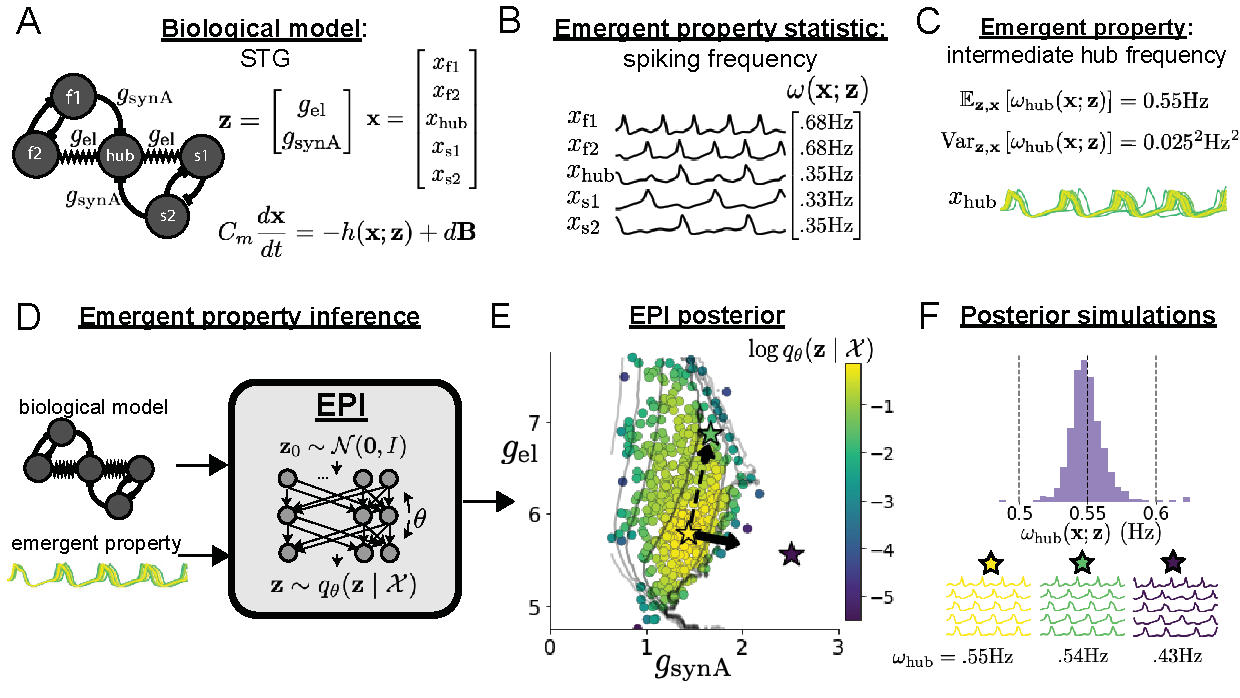
\includegraphics[scale=0.8]{figures/fig1/fig1.pdf}
\end{center}
\caption{\small Emergent property inference (EPI) in the stomatogastric ganglion.  
\textbf{A}. Conductance-based biophysical model of the STG subcircuit.
\textbf{B}. Spiking frequency $\omega(\mathbf{x}; \mathbf{z})$ is an emergent property statistic. 
Simulated at $g_{\text{el}} = 4.5$nS and $g_{\text{synA}} = 3$nS.
\textbf{C}. The emergent property of intermediate hub frequency.
Simulated activity traces are colored by $\log q_{\bm{\theta}}(\mathbf{z} \mid \mathcal{X})$ of generating parameters. (Panel E).
\textbf{D}. For a choice of model and emergent property, emergent property inference (EPI) learns a deep probability distribution of parameters $\mathbf{z}$.
\textbf{E}. The EPI distribution producing intermediate hub frequency.
Samples are colored by log probability density.  
Contours of hub neuron frequency error are shown at levels of $.525$, $.53$, ... $.575$ Hz (dark to light gray away from mean).
Dimension of sensitivity $\mathbf{v}_1$ (solid) and degeneracy $\mathbf{v}_2$ (dashed).
%(Inset) Sensitivity of the system with respect to network syncing along all dimensions of parameter space away from the mode.  
\textbf{F} (Top) The predictive distribution of EPI.
The black and gray dashed lines show the mean and two standard deviations according the emergent property.
(Bottom) Simulations at the starred parameter values.
 }
 \label{fig:STG}
\end{figure}


%Before presenting technical details (in the following section), let us understand emergent property inference schematically:  EPI (Fig. \ref{fig:STG}A gray box) takes, as input, the model and the specified emergent property, and as its output, produces the parameter distribution shown in Figure \ref{fig:STG}B.
Before presenting technical details (in the following section), let us understand emergent property inference schematically.
EPI (Fig. \ref{fig:STG}D) takes, as input, the model and the specified emergent property, and as its output, produces the parameter distribution  EPI (Fig. \ref{fig:STG}E).  
This distribution -- represented for clarity as samples from the distribution -- is a parameter distribution that produces the emergent property. 
%In the STG model, this distribution can be specifically queried to reveal the prototypical parameter configuration for intermediate hub frequency (the mode; Figure \ref{fig:STG}E yellow star), and how it decays based on changes away from the mode.
%Indeed, samples equidistant from the mode along these EPI-identified dimensions of sensitivity ($v_1$) and degeneracy ($v_2$) (Fig. \ref{fig:STG}E, arrows) agree with error contours (Fig. \ref{fig:STG}E contours) and have diminished or preserved hub frequency, respectively (Fig. \ref{fig:STG}F activity traces) (see Section \ref{methods_STG}).

\subsection{A deep generative modeling approach to emergent property inference} \label{results_dgm}
Emergent property inference (EPI) formalizes the three-step procedure of the previous section with deep probability distributions.
%First, we consider the model as a coupled set of differential (and potentially stochastic) equations \cite{gutierrez2013multiple}.  
First, as is typical, we consider the model as a coupled set of differential equations.  
In this STG example, the model activity $\mathbf{x} = \left[ x_{\text{f1}}, x_{\text{f2}}, x_{\text{hub}}, x_{\text{s1}}, x_{\text{s2}} \right]$ is the membrane potential for each neuron, which evolves according to the biophysical conductance-based equation:
\begin{equation} 
\begin{split}
C_m \frac{d\mathbf{x}(t)}{dt} = -h(\mathbf{x}(t); \mathbf{z}) + d\mathbf{B}
 \end{split}
\end{equation} 
where $C_m$=1nF, and $\mathbf{h}$ is a sum of the leak, calcium, potassium, hyperpolarization, electrical, and synaptic currents, all of which have their own complicated dependence on activity $\mathbf{x}$ and parameters $\mathbf{z} = [g_{\text{el}}, g_{\text{synA}}]$, and $d\mathbf{B}$ is white gaussian noise \cite{morris1981voltage, gutierrez2013multiple} (see Section \ref{methods_STG} for more detail).

%Second, we define the emergent property, which as above is network syncing: oscillation of the entire population at an intermediate frequency of our choosing (Figure \ref{fig:STG}A bottom).
%Quantifying this phenomenon is straightforward: we define network syncing to be that each neuron's spiking frequency -- denoted $\omega_{\text{f1}}(\mathbf{x})$, $\omega_{\text{f2}}(\mathbf{x})$, etc. -- is close to an intermediate frequency of 0.53Hz.  
%Mathematically, we achieve this via constraints on the mean and variance of $\omega_\alpha(\mathbf{x})$ for each neuron $\alpha \in \{ \text{f1}, \text{f2}, \text{hub}, \text{s1}, \text{s2} \}$:
%Mathematically, we achieve this via constraints on the mean and variance of the hub neuron spiking frequency.

%Second, we define the emergent property, which as above is ``intermediate hub  frequency" (Figure \ref{fig:STG}C).
%Quantifying this phenomenon is straightforward: we stipulate that the hub neuron's spiking frequency -- denoted $\omega_{\text{hub}}(\mathbf{x})$ is close to a frequency of 0.55Hz.  
%Mathematically, we achieve this with two constraints: by fixing the mean hub frequency over the inferred parameter distribution of $\mathbf{z}$ and its resulting simulations $\mathbf{x}$ to 0.55Hz,
%\begin{equation}\label{eq:EP_STG1}
% \mathbb{E}_{\mathbf{z},\mathbf{x}}\begin{bmatrix} \omega_{\text{hub}}(\mathbf{x}; \mathbf{z}) \end{bmatrix}  ~~=~~  \begin{bmatrix} 0.55 \end{bmatrix}
%\end{equation}
%and requiring that the variance of the hub frequency over the produced simulations is small
%\begin{equation}\label{eq:EP_STG2}
%\text{Var}_{\mathbf{z},\mathbf{x}}\begin{bmatrix} \omega_{\text{hub}}(\mathbf{x}; \mathbf{z}) \end{bmatrix}  ~~=~~  \begin{bmatrix} 0.025^2 \end{bmatrix}.
%\end{equation}
%This level of variance was chosen to be low enough to exclude the fast and slow frequencies of the two populations, but large enough to allow structural examination of the inferred parameter distribution.
%By constraining the means and variances of emergent property statistics over $\mathbf{z}$ as well as the stochasticity of $\mathbf{x}$, we can precisely control the behavior that the inferred distribution that EPI infers.
%In general, an emergent property
%\begin{equation}\label{eq:EP_STG}
%\mathcal{X}:~~ \mathbb{E}_{\mathbf{z},\mathbf{x}}\left[f(\mathbf{x}; \mathbf{z})\right] = \bm{\mu}, \text{Var}_{\mathbf{z},\mathbf{x}}\left[f(\mathbf{x}; \mathbf{z})\right] = \bm{\sigma}^2
%\end{equation}
%defines a collection of datasets with a statistic $f(\mathbf{x}; \mathbf{z})$ (which may be comprised of multiple statistics) and the means $\bm{\mu}$ and variances $\bm{\sigma}^2$ of those statistics over the datasets.
%The choice of $\bm{\sigma}^2$ predicates the degree of variability around the mean $\bm{\mu}$ that is consistent with the emergent property.

Second, we stipulate that our model should produce the emergent property of ``intermediate hub frequency" (Figure \ref{fig:STG}C).
We stipulate that the hub neuron's spiking frequency -- denoted $\omega_{\text{hub}}(\mathbf{x})$ is close to a frequency of 0.55Hz, between that of the slow and fast frequencies.
Mathematically, we define this emergent property with two statistical constraints: that the mean hub frequency is 0.55Hz,
\begin{equation}\label{eq:EP_STG1}
 \mathbb{E}_{\mathbf{z},\mathbf{x}}\begin{bmatrix} \omega_{\text{hub}}(\mathbf{x}; \mathbf{z}) \end{bmatrix}  ~~=~~  0.55 
\end{equation}
and that the variance of the hub frequency is moderate
\begin{equation}\label{eq:EP_STG2}
\text{Var}_{\mathbf{z},\mathbf{x}}\begin{bmatrix} \omega_{\text{hub}}(\mathbf{x}; \mathbf{z}) \end{bmatrix}  ~~=~~   0.025^2.
\end{equation}
The hub neuron frequency is constrained over the distribution of parameters $\mathbf{z}$  and the distribution of the data $\mathbf{x}$ that those parameters produce.
Formally, the emergent property is the collection of these two constraints
\begin{equation}\label{eq:EP_STG}
\mathcal{X}:~~ \mathbb{E}_{\mathbf{z},\mathbf{x}}\left[\omega_{\text{hub}}(\mathbf{x}; \mathbf{z})\right] = 0.55,~~\text{Var}_{\mathbf{z},\mathbf{x}}\left[\omega_{\text{hub}}(\mathbf{x}; \mathbf{z})\right] =0.025^2.
\end{equation}
In general, an emergent property is a collection of first-, second- and higher moments of  statistics that together define the phenomena.

Third, we perform emergent property inference: we find a distribution over parameter configurations $\mathbf{z}$ that produces the emergent property; in other words, they obey the constraints introduced in Equation \ref{eq:EP_STG}.  
This distribution will be chosen from a family of probability distributions $\mathcal{Q} = \left\{ q_{\bm{\theta}}(\mathbf{z}) : \bm{\theta} \in \Theta \right\}$, defined by a deep neural network \cite{rezende2015variational, dinh2017density, papamakarios2017masked} (Figure \ref{fig:STG}D, EPI box).
Deep probability distributions map a simple random variable $\mathbf{z}_0$ through a deep neural network with weights and biases $\bm{\theta}$ to parameters $\mathbf{z} = g_{\bm{\theta}}(\mathbf{z}_0)$ to a suitably complicated distribution (see Section \ref{methods_NF} for more details).
Many distributions in $\mathcal{Q}$ will respect the emergent property constraints, so we select the most random (highest entropy) distribution, which is the same choice made in Bayesian posterior inference (see Section \ref{methods_VI}).
%\cite{jaynes1957information, elsayed2017structure, loaiza2017maximum, savin2017maximum}
In EPI optimization, stochastic gradient steps in $\bm{\theta}$ are taken such that entropy is maximized, and the emergent property $\mathcal{X}$ is produced (see Section \ref{methods_EPI})
The inferred EPI distribution is denoted $q_{\bm{\theta}}(\mathbf{z} \mid \mathcal{X})$, since it is conditioned upon emergent property $\mathcal{X}$. 
This is meant to share the same notation as a posterior distribution $q_{\bm{\theta}}(\mathbf{z} \mid \mathbf{x})$ that is conditioned upon an explicit dataset.

EPI produces parameter distributions that can be queried for scientific insight.
The modes of $q_{\bm{\theta}}(\mathbf{z} \mid \mathcal{X})$ indicate parameter choices exemplary of the emergent property (Fig. \ref{fig:STG}E yellow star).
As probability in the EPI inferred distribution decreases, the emergent property deteriorates.
Perturbing $\mathbf{z}$ along a dimension in which $q_{\bm{\theta}}(\mathbf{z} \mid \mathcal{X})$ does not change will not disturb the emergent property, making this parameter combination \emph{degenerate} with respect to the emergent property.
In contrast, if $\mathbf{z}$ is perturbed along a dimension that strongly decreases $q_{\bm{\theta}}(\mathbf{z} \mid \mathcal{X})$, we call that parameter combination \emph{sensitive}.
By querying the second order derivative (Hessian) of $\log q_{\bm{\theta}}(\mathbf{z} \mid \mathcal{X})$ at a mode, we can quantitatively identify how sensitive (or robust) each eigenvector is by its eigenvalue; the more negative the eigenvalue, the more sensitive.
Indeed, samples equidistant from the mode along these EPI-identified dimensions of sensitivity ($v_1$, smaller eigenvalue) and robustness ($v_2$, greater eigenvalue) (Fig. \ref{fig:STG}E, arrows) agree with error contours (Fig. \ref{fig:STG}E contours) and have diminished or preserved hub frequency, respectively (Fig. \ref{fig:STG}F activity traces).
Once an EPI distribution has been inferred, this Hessian calculation requires trivial computation (when the correct architecture class is chosen, see Section \ref{methods_NF}).

In the following sections, we demonstrate EPI on three neural circuit models across ranges of biological realism, neural system function, and network scale.
First, we demonstrate the superior scalability of EPI compared to alternative techniques by inferring high-dimensional distributions of recurrent neural network (RNN) connectivities that exhibit amplified, yet stable responses.
Also in this RNN example, we emphasize that EPI is the only technique that controls the predictions made by the inferred parameter distribution.
Next, in a model of primary visual cortex \cite{litwin2016inhibitory, palmigiano2020structure}, we show how EPI captures a curved manifold of parametric degeneracy, revealing how input variability across neuron types affects the excitatory population.
Finally, in a model of superior colliculus \cite{duan2018collicular}, we used EPI to capture multiple parametric regimes of task switching, and queried the dimensions of sensitivity ($\mathbf{v}_1(\mathbf{z})$) to mechanistically characterize each regime.

%Third, we perform emergent property inference: we find a distribution over parameter configurations $\mathbf{z}$, and insist that samples from this distribution produce the emergent property; in other words, they obey the constraints introduced in Equation \ref{eq:EP_STG}.  
%This distribution will be chosen from a family of probability distributions $\mathcal{Q} = \left\{ q_{\bm{\theta}}(\mathbf{z}) : \bm{\theta} \in \Theta \right\}$, defined by a deep generative distribution of the normalizing flow class \cite{rezende2015variational, dinh2017density, papamakarios2017masked} -- neural networks which transform a simple distribution into a suitably complicated distribution (as is needed here).  
%This deep distribution is represented in Figure \ref{fig:STG}E (see Section \ref{methods_EPI}).  
%Then, mathematically, we must solve the following optimization program: 
%\begin{equation} \label{eq:EPI}
%\begin{split}
%q_{\bm{\theta}}(\mathbf{z} \mid \mathcal{X}) ~~=~~ &\argmax_{q_{\bm{\theta}} \in \mathcal{Q}} H(q_{\bm{\theta}}(\mathbf{z})) \\
%&\text{  s.t.  } ~\mathcal{X}:~~ \mathbb{E}_{\mathbf{z},\mathbf{x}}\left[f(\mathbf{x}; \mathbf{z})\right] = \bm{\mu}, \text{Var}_{\mathbf{z},\mathbf{x}}\left[f(\mathbf{x}; \mathbf{z})\right] = \bm{\sigma}^2 \\
%\end{split}
%\end{equation}
%where $f(\mathbf{x}, \mathbf{z}), \bm{\mu}$, and $\bm{\sigma}$ are defined as in Equation \ref{eq:EP}.
%According to the emergent property of interest, $f(\mathbf{x}, \mathbf{z})$ may contain multiple statistics, in which case the mean and variance vectors $\bm{\mu}$ and $\bm{\sigma}^2$ match this dimension.
%Finally, we recognize that many distributions in $\mathcal{Q}$ will respect the emergent property constraints, so we select that which has maximum entropy.
%This principle, captured in Equation \ref{eq:EPI} by the primal objective $H$, identifies parameter distributions with minimal assumptions beyond some chosen structure \cite{jaynes1957information, elsayed2017structure, loaiza2017maximum, savin2017maximum}.
%Such a normative principle of maximum entropy, which is also that of Bayesian inference, naturally fits with our scientific objective of reasoning about parametric sensitivity and robustness. 
%The recovered distribution of EPI is as variable as possible along each parametric manifold such that it produces the emergent property.

%EPI optimizes the weights and biases $\bm{\theta}$ of the deep network (which induces the probability distribution) by iteratively solving Equation \ref{eq:EPI}. 
%The optimization is complete when the sampled models with parameters $\mathbf{z} \sim q_{\bm{\theta}}(z \mid \mathcal{X})$ produce activity consistent with the specified emergent property (Fig. S4).
%%Such convergence is evaluated with a hypothesis test that the mean of each emergent property statistic is not different than its emergent property value (see Section \ref{methods_AL_opt}). 
%Such convergence is evaluated with a hypothesis test that the means and variances of each emergent property statistic are not different than their constrained values (see Section \ref{methods_AL_opt}). 
%Further validation of EPI is available in the supplementary materials, where we analyze a simpler model for which ground-truth statements can be made (Section \ref{methods_2DLDS}).

%In relation to broader methodology, inspection of the EPI objective reveals a natural relationship to posterior inference.
%Specifically, EPI executes a novel variant of  Bayesian inference with a uniform prior and a gaussian likelihood on the emergent property statistic (see Section \ref{methods_ME_EF}).
%A key advantage of EPI over established Bayesian inference is that the predictions made by the inferred distribution are constrained to produce the specified emergent property.

%The major scientific value of EPI is in the rich, queryable structure of these deep probability distributions.
%The probabilities of $q_{\bm{\theta}}(\mathbf{z} \mid \mathcal{X})$ are the densities of these parameters in the distribution producing the emergent property.
%The greatest probabilities (the modes) indicate prototypical parameter configurations, and the manner in which probabilities change away from the modes shows how different parameter combinations preserve or diminish the emergent property.
%The dimensions of greatest sensitivity (e.g. Fig. 1E solid arrow) or degeneracy (e.g. Fig. 1E dashed arrow) can be measured directly from the second order derivative of $\log q_{\bm{\theta}}(\mathbf{z} \mid \mathcal{X})$ called the ``Hessian."
%Around the mode, eigenvalues of the Hessian are negative; probabilities decrease locally in all directions away from the mode.
%The eigenvector with most negative eigenvalue is the parameter combination causing probability to decrease the fastest, making it the most sensitive dimension.
%Likewise, the flattest eigenvector, corresponding to the least negative eigenvalue, points in the most degenerate dimension.
%Once an EPI distribution has been inferred, this second order derivative requires trivial computation (when correct architecture class is chosen, see Section \ref{methods_NF}).

\subsection{Scaling inference of RNN connectivity with EPI} \label{results_LRRNN}
Transient amplification is a hallmark of neural activity throughout cortex, and is often thought to be intrinsically generated by recurrent connectivity in the responding cortical area \cite{murphy2009balanced, hennequin2014optimal, bondanelli2019population}.
It has been shown that to generate such amplified, yet stabilized responses, the connectivity of RNNs must be non-normal \cite{goldman2009memory, murphy2009balanced}, and satisfy additional constraints \cite{bondanelli2020coding}.
In theoretical neuroscience, RNNs are optimized and then examined to show how dynamical systems could execute a given computation \cite{sussillo2014neural, barak2017recurrent}, but such biologically realistic constraints on connectivity are  ignored during optimization for practical reasons.
In general, access to distributions of connectivity adhering to theoretical criteria like stable amplification, chaotic fluctuations \cite{sompolinsky1988chaos}, or low tangling \cite{russo2018motor} would add scientific value and context to existing research with RNNs.
Here, we use EPI to learn RNN connectivities producing stable amplification, and demonstrate the superior scalability and efficiency of EPI to alternative approaches.
\begin{figure}
\begin{center}
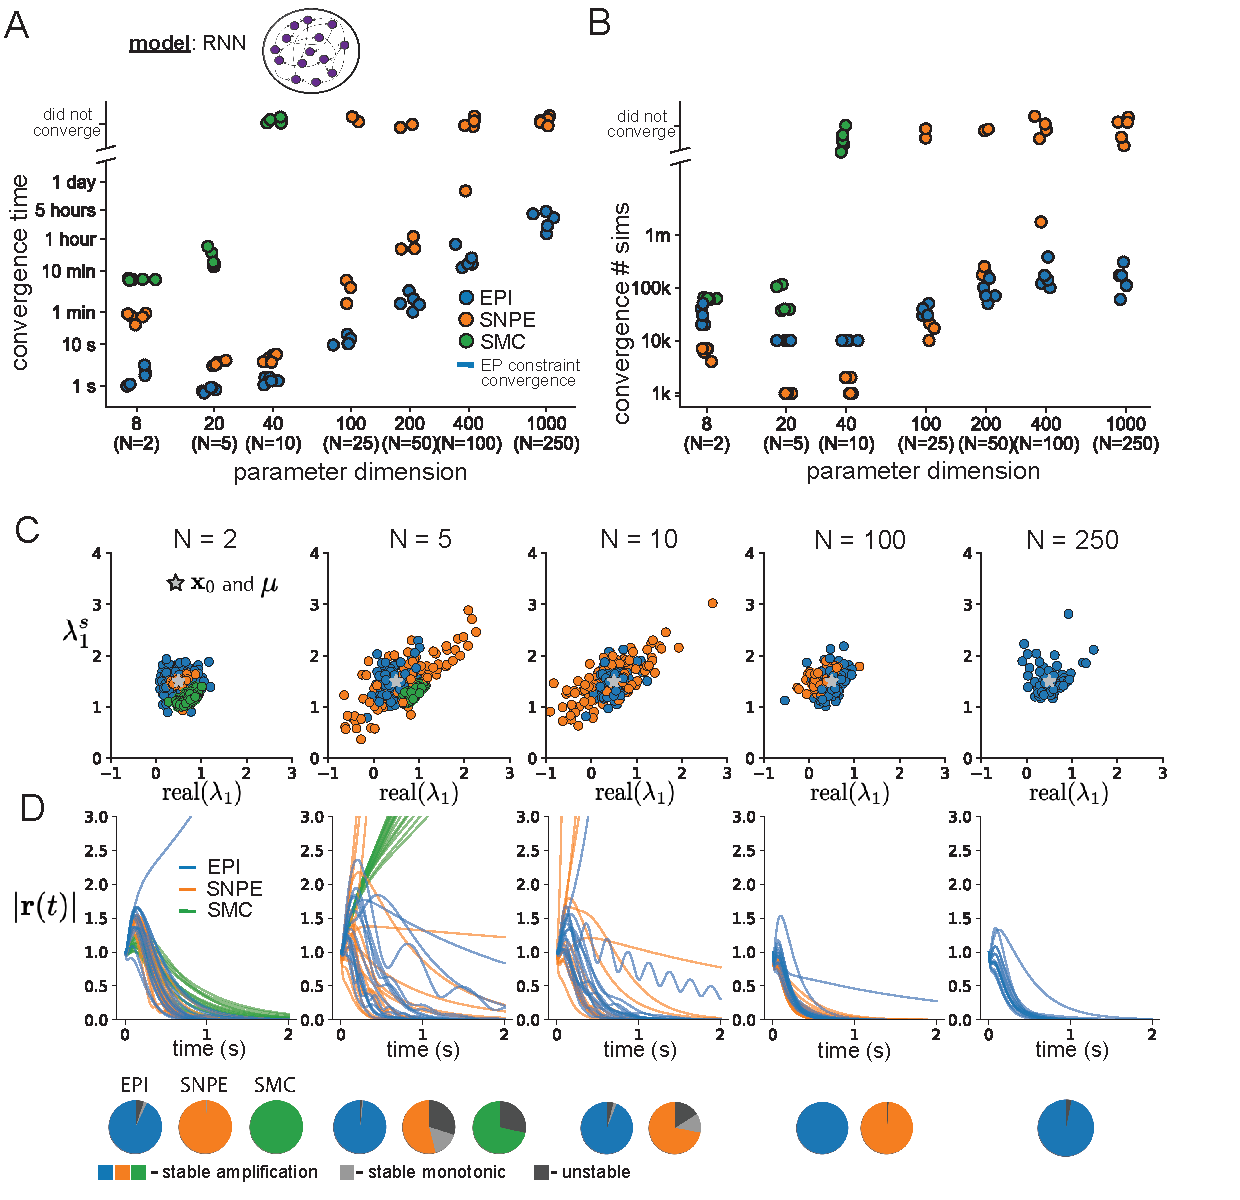
\includegraphics[scale=.8]{figures/fig2/fig2.pdf}
\end{center}
\caption{\small 
\textbf{A}. Wall time of EPI (blue), SNPE (orange), and SMC-ABC (green) to converge on RNN connectivities producing stable amplification.  
Each dot shows convergence time for an individual random seed.
For reference, the mean wall time for EPI to achieve its full constraint convergence (means and variances) is shown (blue line).
\textbf{B}. Simulation count of each algorithm to achieve convergence. Same conventions as A.
\textbf{C}. The predictive distributions of connectivities inferred by EPI (blue), SNPE (orange), and SMC-ABC (green), with reference to $\mathbf{x}_0 = \bm{\mu}$ (gray star).
\textbf{D}. Simulations of networks inferred by each method ($\tau=100ms$).  Each trace (15 per algorithm) corresponds to simulation of one $z$.  (Below) Ratio of obtained samples producing stable amplification, monotonic decay, and instability.
}
\label{fig:LRRNN}
\end{figure}

We consider a rank-2 RNN with $N$ neurons having connectivity $W = UV^\top$
 and dynamics
 \begin{equation}
 \tau \dot{\mathbf{x}} = -\mathbf{x} + W\mathbf{x},
 \end{equation}
where $U = \begin{bmatrix} \mathbf{u}_1 & \mathbf{u}_2 \end{bmatrix} + g \chi^{(U)}$, $V = \begin{bmatrix} \mathbf{v}_1 & \mathbf{v}_2 \end{bmatrix} + g\chi^{(V)}$, $\mathbf{u}_1 \mathbf{u}_2, \mathbf{v}_1, \mathbf{v}_2 \in \left[-1, 1 \right]^N$, and $\chi^{(U)}_{i,j}, \chi^{(V)}_{i,j} \sim \mathcal{N}(0, 1)$.
We infer connectivity parameterizations $\mathbf{z} = \left[\mathbf{u}_1^\top, \mathbf{u}_2^\top, \mathbf{v}_1^\top, \mathbf{v}_2^\top \right]^\top$   that produce stable amplification.
Two conditions are necessary and sufficient for RNNs to exhibit stable amplification \cite{bondanelli2020coding}:  $\text{real}(\lambda_1) < 1$ and
$\lambda^s_1 > 1$, where $\lambda_1$ is the eigenvalue of $W$ with greatest real part and $\lambda^s$ is the maximum eigenvalue of $W^s = \frac{W + W^\top}{2}$.
RNNs  with $\text{real}(\lambda_1) = 0.5 \pm 0.5$ and $\lambda_1^s = 1.5 \pm 0.5$ will be stable with modest decay rate ($\text{real}(\lambda_1)$ close to its upper bound of 1) and exhibit modest amplification ($\lambda_1^s$ close to its lower bound of 1).
 EPI can naturally condition on this emergent property
\begin{equation}\label{eq:EP_LRRNN}
\begin{split}
\mathcal{X} ~~:~~ \mathbb{E}_{\mathbf{z}, \mathbf{x}} \begin{bmatrix} \text{real}(\lambda_1) \\ \lambda^s_1 \end{bmatrix} &= \begin{bmatrix} 0.5 \\ 1.5 \end{bmatrix} \\
\text{Var}_{\mathbf{z}, \mathbf{x}} \begin{bmatrix} \text{real}(\lambda_1) \\ \lambda^s_1 \end{bmatrix} &= \begin{bmatrix} 0.25^2 \\ 0.25^2 \end{bmatrix},
\end{split}
\end{equation}
under the notion that variance constraints with standard deviation 0.25 predicate that the vast majority of samples (those within two standard deviations) are within the specified ranges.

For comparison, we infer the parameters $\mathbf{z}$ likely to produce stable amplification using two alternative simulation-based inference approaches.
We ran sequential Monte Carlo approximate Bayesian computation (SMC-ABC) \cite{sisson2007sequential} and sequential neural posterior estimation (SNPE) \cite{gonccalves2019training} with observation $\mathbf{x}_0 = \bm{\mu}$.
SMC-ABC is a rejection sampling approach that SMC techniques to improve efficiency, and SNPE approximates posteriors with deep probability distributions using a two-network architecture (see Section \ref{methods_related}).
Unlike EPI, these statistical inference techniques do not constrain the statistics of the predictive distribution, and these predictions of the inferred posteriors are typically affected by model characteristics (e.g. $N$ and $g$, Fig. \ref{fig:RNN2}).
To compare the efficiency of these different techniques, we measured the time and number of simulations necessary for the distance of the predictive mean to be less than 0.5 from $\bm{\mu} = \mathbf{x}_0$ (see Section \ref{methods_RNN}).

As the number of neurons $N$ in the RNN is scaled, and thus the dimension of the parameter space $\mathbf{z} \in [-1, 1]^{4N}$, we see that EPI converges at greater speed and at greater dimension than SMC-ABC and SNPE (Fig. \ref{fig:LRRNN}A).
It also becomes most efficient to use EPI in terms of simulation count at $N=50$ (Fig. \ref{fig:LRRNN}B).
It is well known that ABC techniques struggle in dimensions greater than about 30 \cite{sisson2018handbook}, yet we were careful to assess the scalability of the more comparable approach SNPE.
Between EPI and SNPE, we closely controlled the number of parameters in deep probability distributions by dimensionality (Fig. \ref{fig:RNN1}), and tested more aggressive SNPE hyperparameterizations when SNPE failed to converge (Fig. \ref{fig:RNN3}).
From this analysis, we see that deep inference techniques EPI and SNPE are far more amenable to inference of high dimensional parameter distributions than rejection sampling techniques like SMC-ABC, and that EPI outperforms SNPE in both criteria in high dimensions.

No matter the number of neurons, EPI always produces connectivity distributions with mean and variance of $\text{real}(\lambda_1)$ and $\lambda_1^s$ according to $\mathcal{X}$ (Fig. \ref{fig:LRRNN}C, blue).
For the dimensionalities in which SMC-ABC is tractable, the inferred parameters are concentrated and offset from $\mathbf{x}_0$ (Fig. \ref{fig:LRRNN}C, green).
When using SNPE the predictions of the inferred parameters are highly concentrated at some RNN sizes and widely varied in others (Fig. \ref{fig:LRRNN}C, orange).
We see these properties reflected in simulations from the inferred distributions: EPI produces a consistent variety of stable, amplified activity norms $|r(t)|$, SMC-ABC produces a limited variety of responses, and the changing variety of responses from SNPE emphasizes the control of EPI on parameter predictions.

EPI outperforms SNPE in high dimensions by using gradient information (from $\nabla_\mathbf{z} f(\mathbf{x}; \mathbf{z}) = \nabla_\mathbf{z} [\text{real}(\lambda_1), \lambda_1^s]^\top$) on each iteration of optimization.
This agrees with recent speculation that such gradient information could improve the efficiency of simulation-based inference techniques \cite{cranmer2020frontier}.
Since gradients of the emergent property statistics are necessary in EPI optimization, gradient tractabillity is a key criteria when determining the suitability of a simulation-based inference technique.
Evidenced by this analysis, EPI is a clear choice for inferring high dimensional parameter distributions when the emergent property gradient is efficiently calculated.
This can be invaluable for understanding how RNNs produce complex emergent phenomena.
Even with a high degree of biophysical realism and expensive emergent property gradients, EPI was run successfully on intermediate hub frequency in a 5-neuron subcircuit model of the STG (Section \ref{results_motivating}).
However, conditioning on the pyloric rhythm \cite{marder1992dynamic} in a model of the pyloric subnetwork model \cite{prinz2004similar} proved to be prohibitive with EPI.
The pyloric subnetwork requires many time steps for simulation and many key emergent property statistics (e.g. burst duration and phase gap) are not calculable or easily approximated with differentiable functions.
In such cases, gradient-free approaches like SNPE have proved to be a powerful option \cite{gonccalves2019training}.
In the next two sections, we use EPI for novel scientific insight by examining the structure of inferred distributions.

%\section{Discussion}
%\subsection{EPI is a general tool for theoretical neuroscience} 
%Biologically realistic models of neural circuits are comprised of complex nonlinear differential equations, making traditional theoretical analysis and statistical inference intractable. 
%We advance the capabilities of statistical inference in theoretical neuroscience by presenting EPI, a deep inference methodology for learning parameter distributions of theoretical models performing neural computation.
%We have demonstrated the utility of EPI on biological models (STG), intermediate-level models of interacting genetically- and functionally-defined neuron-types (V1, SC), and the most abstract of models (RNNs).  
%We are able to condition both deterministic and stochastic models on low-level emergent properties like spiking frequency of membrane potentials, as well as high-level cognitive function like posterior conditioning.
%Technically, EPI is tractable when the emergent property statistics are continuously differentiable with respect to the model parameters, which is very often the case; this emphasizes the general applicability of EPI.
%
%In this study, we have focused on applying EPI to low dimensional parameter spaces of models with low dimensional dynamical states.
%These choices were made to present the reader with a series of  interpretable conclusions, which is more challenging in high dimensional spaces.
%In fact, EPI should scale reasonably to high dimensional parameter spaces, as the underlying technology has produced state-of-the-art performance on high-dimensional tasks such as texture generation \cite{loaiza2017maximum}.
%Of course, increasing the dimensionality of the dynamical state of the model makes optimization more expensive, and there is a practical limit there as with any machine learning approach.
%Although, theoretical approaches (e.g. \cite{mastrogiuseppe2018linking}) can be used to reason about the wholistic activity of such high dimensional systems by introducing some degree of additional structure into the model.

%%%%%%%%%%%%%%%%%%%%%%%%%%%%
\subsection{EPI reveals how noisy input across neuron-types governs excitatory variability in a V1 model} \label{results_V1}

\begin{figure}
\vspace{-1cm}
\begin{center}
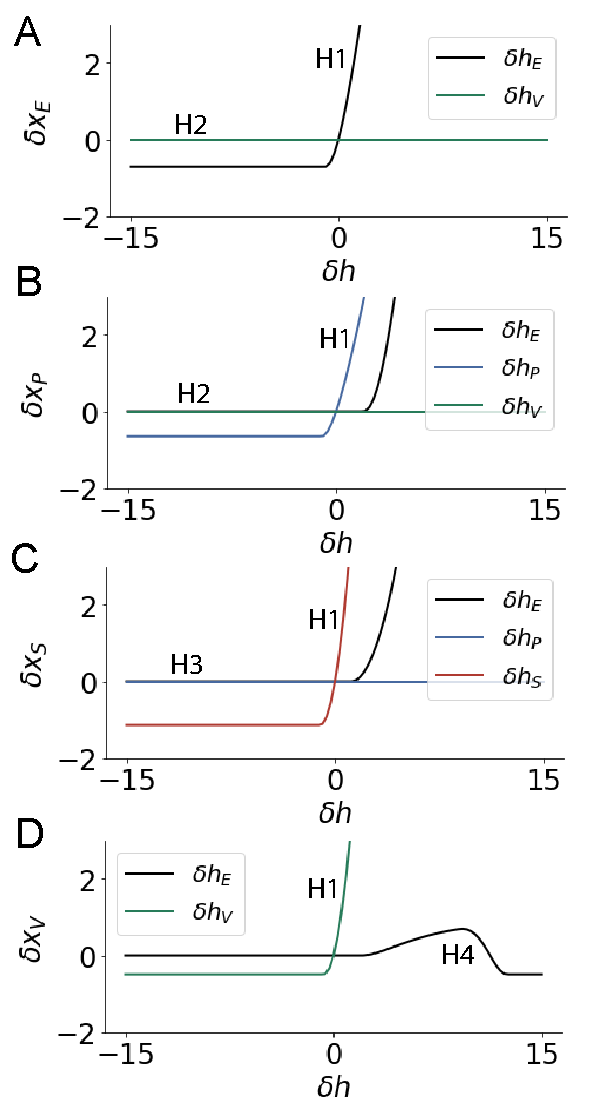
\includegraphics[scale=0.8]{figures/fig3/fig3.pdf}
\end{center}
\vspace{-1cm}
\caption{\small Emergent property inference in the stochastic stabilized supralinear network (SSSN)
\textbf{A}.  Four-population model of primary visual cortex with excitatory (black), parvalbumin (blue), somatostatin (red), and VIP (green) neurons (excitatory and inhibitory projections filled and unfilled, respectively).   
Some neuron-types largely do not form synaptic projections to others ($|W_{\alpha_1, \alpha_2})| < 0.025$).
Each neural population receives a baseline input $\mathbf{h}_b$, and the E- and P-populations also receive a contrast-dependent input $\mathbf{h}_c$.
Additionally, each neural population receives a slow noisy input $\bm{\epsilon}$.
\textbf{B}. Transient network responses of the SSSN model. Traces are independent trials with varying initialization $\mathbf{x}(0)$ and noise $\bm{\epsilon}$. 
\textbf{C}. Mean (solid line) and standard deviation $s_E(\mathbf{x}; \mathbf{z})$ (shading)  across 100 trials.
\textbf{D}. EPI distribution of noise parameters $\mathbf{z}$ conditioned on E-population variability.
The EPI predictive distribution of $s_E(\mathbf{x}; \mathbf{z})$ is show on the bottom-left.
\textbf{E}. (Top) Enlarged visualization of the $\sigma_E$-$\sigma_P$ marginal distribution of EPI $q_{\bm{\theta}}(\mathbf{z} \mid \mathcal{X}(5\text{ Hz})$ and $q_{\bm{\theta}}(\mathbf{z} \mid \mathcal{X}(10\text{ Hz})$.
Each black dot shows the mode at each $\sigma_P$.
The arrows show the most sensitive dimensions of the Hessian evaluated at these modes.
\textbf{F}. The predictive distributions of $\sigma_E^2 + \sigma_P^2$ of each inferred distribution $q_{\bm{\theta}}(\mathbf{z} \mid \mathcal{X}(5\text{ Hz})$ and $q_{\bm{\theta}}(\mathbf{z} \mid \mathcal{X}(10\text{ Hz})$.
}
 \label{fig:V1}
\end{figure}

Dynamical models of excitatory (E) and inhibitory (I) populations with supralinear input-output function have succeeded in explaining a host of experimentally documented phenomena.
In a regime characterized by inhibitory stabilization of strong recurrent excitation, these models give rise to paradoxical responses \cite{tsodyks1997paradoxical}, selective amplification  \cite{goldman2009memory, murphy2009balanced}, surround suppression \cite{ozeki2009inhibitory} and normalization \cite{rubin2015stabilized}. 
Despite their strong predictive power, E-I circuit models rely on the assumption that inhibition can be studied as an indivisible unit. 
However, experimental evidence shows that inhibition is composed of distinct elements -- parvalbumin (P), somatostatin (S), VIP (V) --
composing 80\% of GABAergic interneurons in V1 \cite{markram2004interneurons, rudy2011three, tremblay2016}, and that these inhibitory cell types follow specific connectivity patterns (Fig. \ref{fig:V1}A) \cite{pfeffer2013inhibition}.
%Recent theoretical advances \cite{litwin2016inhibitory, GarciaDelMolino2017, Chen2019},  have only started to address the consequences of this multiplicity in the dynamics of V1, strongly relying on linear theoretical tools. 
While research has shown that V1 only shares specific dimensions of neuronal variability with downstream areas \cite{semedo2019cortical}, the role played by recurrent dynamics and the connectivity across neuron-type populations is not understood.
Here, in a model of V1 with biologically realistic connectivity, we use EPI to show how the structure of input across neuron types affects the variability of the excitatory population -- the population largely responsible for projecting to other brain areas \cite{felleman1991distributed}.

We considered response variability of a nonlinear dynamical V1 circuit model (Fig. \ref{fig:V1}A) with a state comprised of each neuron-type population's rate $\mathbf{x} = \left[x_E, x_P , x_S, x_V \right]^\top$.
Each population receives recurrent input $W \mathbf{x}$, where $W$ is the effective connectivity estimated from post-synaptic potential and connectivity rate measurements (see Section \ref{methods_V1}).
Each population also experiences an external input $\mathbf{h}$, which determines population rate via supralinear nonlinearity $\phi(\cdot) = \left[\cdot \right]^2_+$.
There is also an additive noisy input $\bm{\epsilon}$ parameterized by variances for each neuron type population $\bm{\sigma}^2 = \left[ \sigma_E^2, \sigma_P^2, \sigma_S^2, \sigma_V^2\right]$.
This noise has a slower dynamical timescale $\tau_{\text{noise}} > \tau$ than the population rate, allowing fluctuations around a stimulus-dependent steady-state (Fig. \ref{fig:V1}B).
This model is the stochastic stabilized supralinear network (SSSN) \cite{hennequin2018dynamical} 
\begin{equation}
    \tau \frac{d\mathbf{x}}{dt} = -\mathbf{x} +\phi(W\mathbf{x} + \mathbf{h} + \bm{\epsilon}).
\end{equation}
generalized to have multiple inhibitory neuron types, and introduces stochasticity to previous four neuron-type models of V1 \cite{litwin2016inhibitory}.
Stochasticity and inhibitory multiplicity introduce substantial complexity to mathematical derivations (see Section \ref{methods_V1_complexity}) motivating the treatment of this model with EPI.
Here, we consider fixed weights $W$ and input $\mathbf{h}$ \cite{palmigiano2020structure}, and study the effect of input variability $\mathbf{z} = [\sigma_E, \sigma_P, \sigma_S, \sigma_V]^\top$ on excitatory variability.

We quantify levels $y$ of E-population variability with the emergent property
\begin{equation}\label{eq:EP_V1}
\begin{split}
\mathcal{X}(y) ~~:~~  \mathbb{E}_{\mathbf{z}}\begin{bmatrix} s_E(\mathbf{x}; \mathbf{z}) \end{bmatrix}  &~~=~~ y \\ 
 \text{Var}_{\mathbf{z}}\begin{bmatrix} s_E(\mathbf{x}; \mathbf{z}) \end{bmatrix}  &~~=~~  1 \text{Hz}^2,
\end{split}
\end{equation}
where $s_E(\mathbf{x}; \mathbf{z})$ is the standard deviation of the stochastic $E$-population response about its steady state (Fig. \ref{fig:V1}C).
In the following analyses, we compare levels of 5Hz and 10Hz, and select 1 Hz$^2$ variance such that the two emergent properties do not overlap in $s_E(\mathbf{z}; \mathbf{x})$.

First, we ran EPI to obtain parameter distribution $q_{\bm{\theta}}(\mathbf{z} \mid \mathcal{X}(5\text{ Hz}))$ producing E-population variability around 5 Hz (Fig. \ref{fig:V1}D).
From the marginal distribution of $\sigma_E$ and $\sigma_P$ (Fig. \ref{fig:V1}D, top-left), we can see that $s_E(\mathbf{x}; \mathbf{z})$ is sensitive to various combinations of $\sigma_E$ and $\sigma_P$.
Alternatively, both $\sigma_S$ and $\sigma_V$ are degenerate with respect to $s_E(\mathbf{x}; \mathbf{z})$ evidenced by the high variability in those dimensions (Fig. \ref{fig:V1}D, bottom-right).
Together, these observations imply a curved path with respect to $s_E(\mathbf{x}; \mathbf{z})$ of 5 Hz, which is indicated by the modes along $\sigma_P$ (Fig. \ref{fig:V1}E).

Figure \ref{fig:V1}E suggests a quadratic relationship in E-population fluctuations and the standard deviation of E- and P-population input; as the square of either $\sigma_E$ or $\sigma_P$ increases, the other compensatorily decreases to preserve the level of $s_E(\mathbf{x}; \mathbf{z})$.
This quadratic relationship is preserved at greater level of E-population variability $\mathcal{X}(10\text{ Hz})$ (Fig. \ref{fig:V1}E).
Indeed, the sum of squares of $\sigma_E$ and $\sigma_P$ is larger in $q_{\bm{\theta}}(\mathbf{z} \mid \mathcal{X}(10\text{ Hz}))$ than $q_{\bm{\theta}}(\mathbf{z} \mid \mathcal{X}(5\text{ Hz}))$ (Fig \ref{fig:V1}F, $p < 1 \times 10^{-10}$), while the sum of squares of $\sigma_S$ and $\sigma_V$ are not significantly different in the two EPI distributions (Fig. \ref{fig:V1_3}, $p=.40$), in which parameters were bounded from 0 to 0.5.
The strong interactive influence of E- and P-population input variability on excitatory varability is intriguing, since this circuit exhibits a paradoxical effect in the P-population (and no other inhibitory types) (Fig. \ref{fig:V1_3}), meaning that the E-population is P-stabilized.
Future research may uncover a link between the population of network stabilization and compensatory interactions governing excitatory variability.

EPI revealed the quadratic dependence of excitatory variability on input variability to the E- and P-populations, as well as its independence to input from the other two inhibitory populations.
We show that with each neuron-type population added to this E-I model, calculations of excitatory variability with respect to noise parameters become unruly and challenging to work with (see Section \ref{methods_V1_complexity}).
This emphasizes the value of streamlined methods for gaining understanding about theoretical models when mathematical analysis becomes onerous or impractical.
While EPI can be used to investigate fundamental aspects of sensory processing, in the next section, we use the probabilistic tools of EPI to identify and characterize two distinct parametric regimes of a neural circuit executing a computation, and then relate these insights to  behavioral experiments.

%%%%%%%%%%%%%%%%%%%%%%%%
\subsection{EPI identifies two regimes of rapid task switching} \label{results_SC}
It has been shown that rats can learn to switch from one behavioral task to the next on randomly interleaved trials \cite{duan2015requirement}, and an important question is what types of neural connectivity allow this ability.
In this experimental setup, rats were explicitly cued on each trial to either orient towards a visual stimulus in the Pro (P) task or orient away from a visual stimulus in the Anti (A) task (Fig. \ref{fig:SC}A). 
Neural recordings in superior colliculus (SC) exhibited two populations of neurons that represented task context (Pro or Anti).
Furthermore, Pro/Anti neurons in each hemisphere were strongly correlated with the animal's decision \cite{duan2018collicular}.
These results motivated a model of SC that is a four-population dynamical system with functionally-defined neuron-types.
Here, our goal is to understand how connectivity in this circuit model governs the ability to perform rapid task switching: to respond with satisfactory accuracy in both tasks on randomly interleaved trials.

In this SC model, there are Pro- and Anti-populations in each hemisphere (left (L) and right (R)) with activity variables $\mathbf{x} = [x_{LP}, x_{LA}, x_{RP}, x_{RA}]^\top$.
The connectivity of these populations is parameterized by self $sW$, vertical $vW$, diagonal $dW$ and horizontal $hW$ connections (Fig. \ref{fig:SC}B).
The input $\mathbf{h}$ is comprised of a positive cue-dependent signal to the Pro or Anti populations, a positive stimulus-dependent input to either the Left or Right populations, and a choice-period input to the entire network (see Section \ref{methods_SC}).
Model responses are bounded from 0 to 1 as a function $\phi$ of an internal variable $\mathbf{u}$
\begin{equation}
\begin{split}
\tau \frac{d\mathbf{u}}{dt} &= -\mathbf{u} + W\mathbf{x} + \mathbf{h} + d\mathbf{B} \\
\mathbf{x} &= \phi(\mathbf{u}).
\end{split}
\end{equation}
The model responds to the side with greater Pro neuron activation; e.g. the response is left if $x_{LP} > x_{RP}$ at the end of the trial.  
Here, we use EPI to determine the network connectivity $\mathbf{z} = [sW, vW, dW, hW]^{\top}$ that produces rapid task switching.

\begin{figure}
\begin{center}
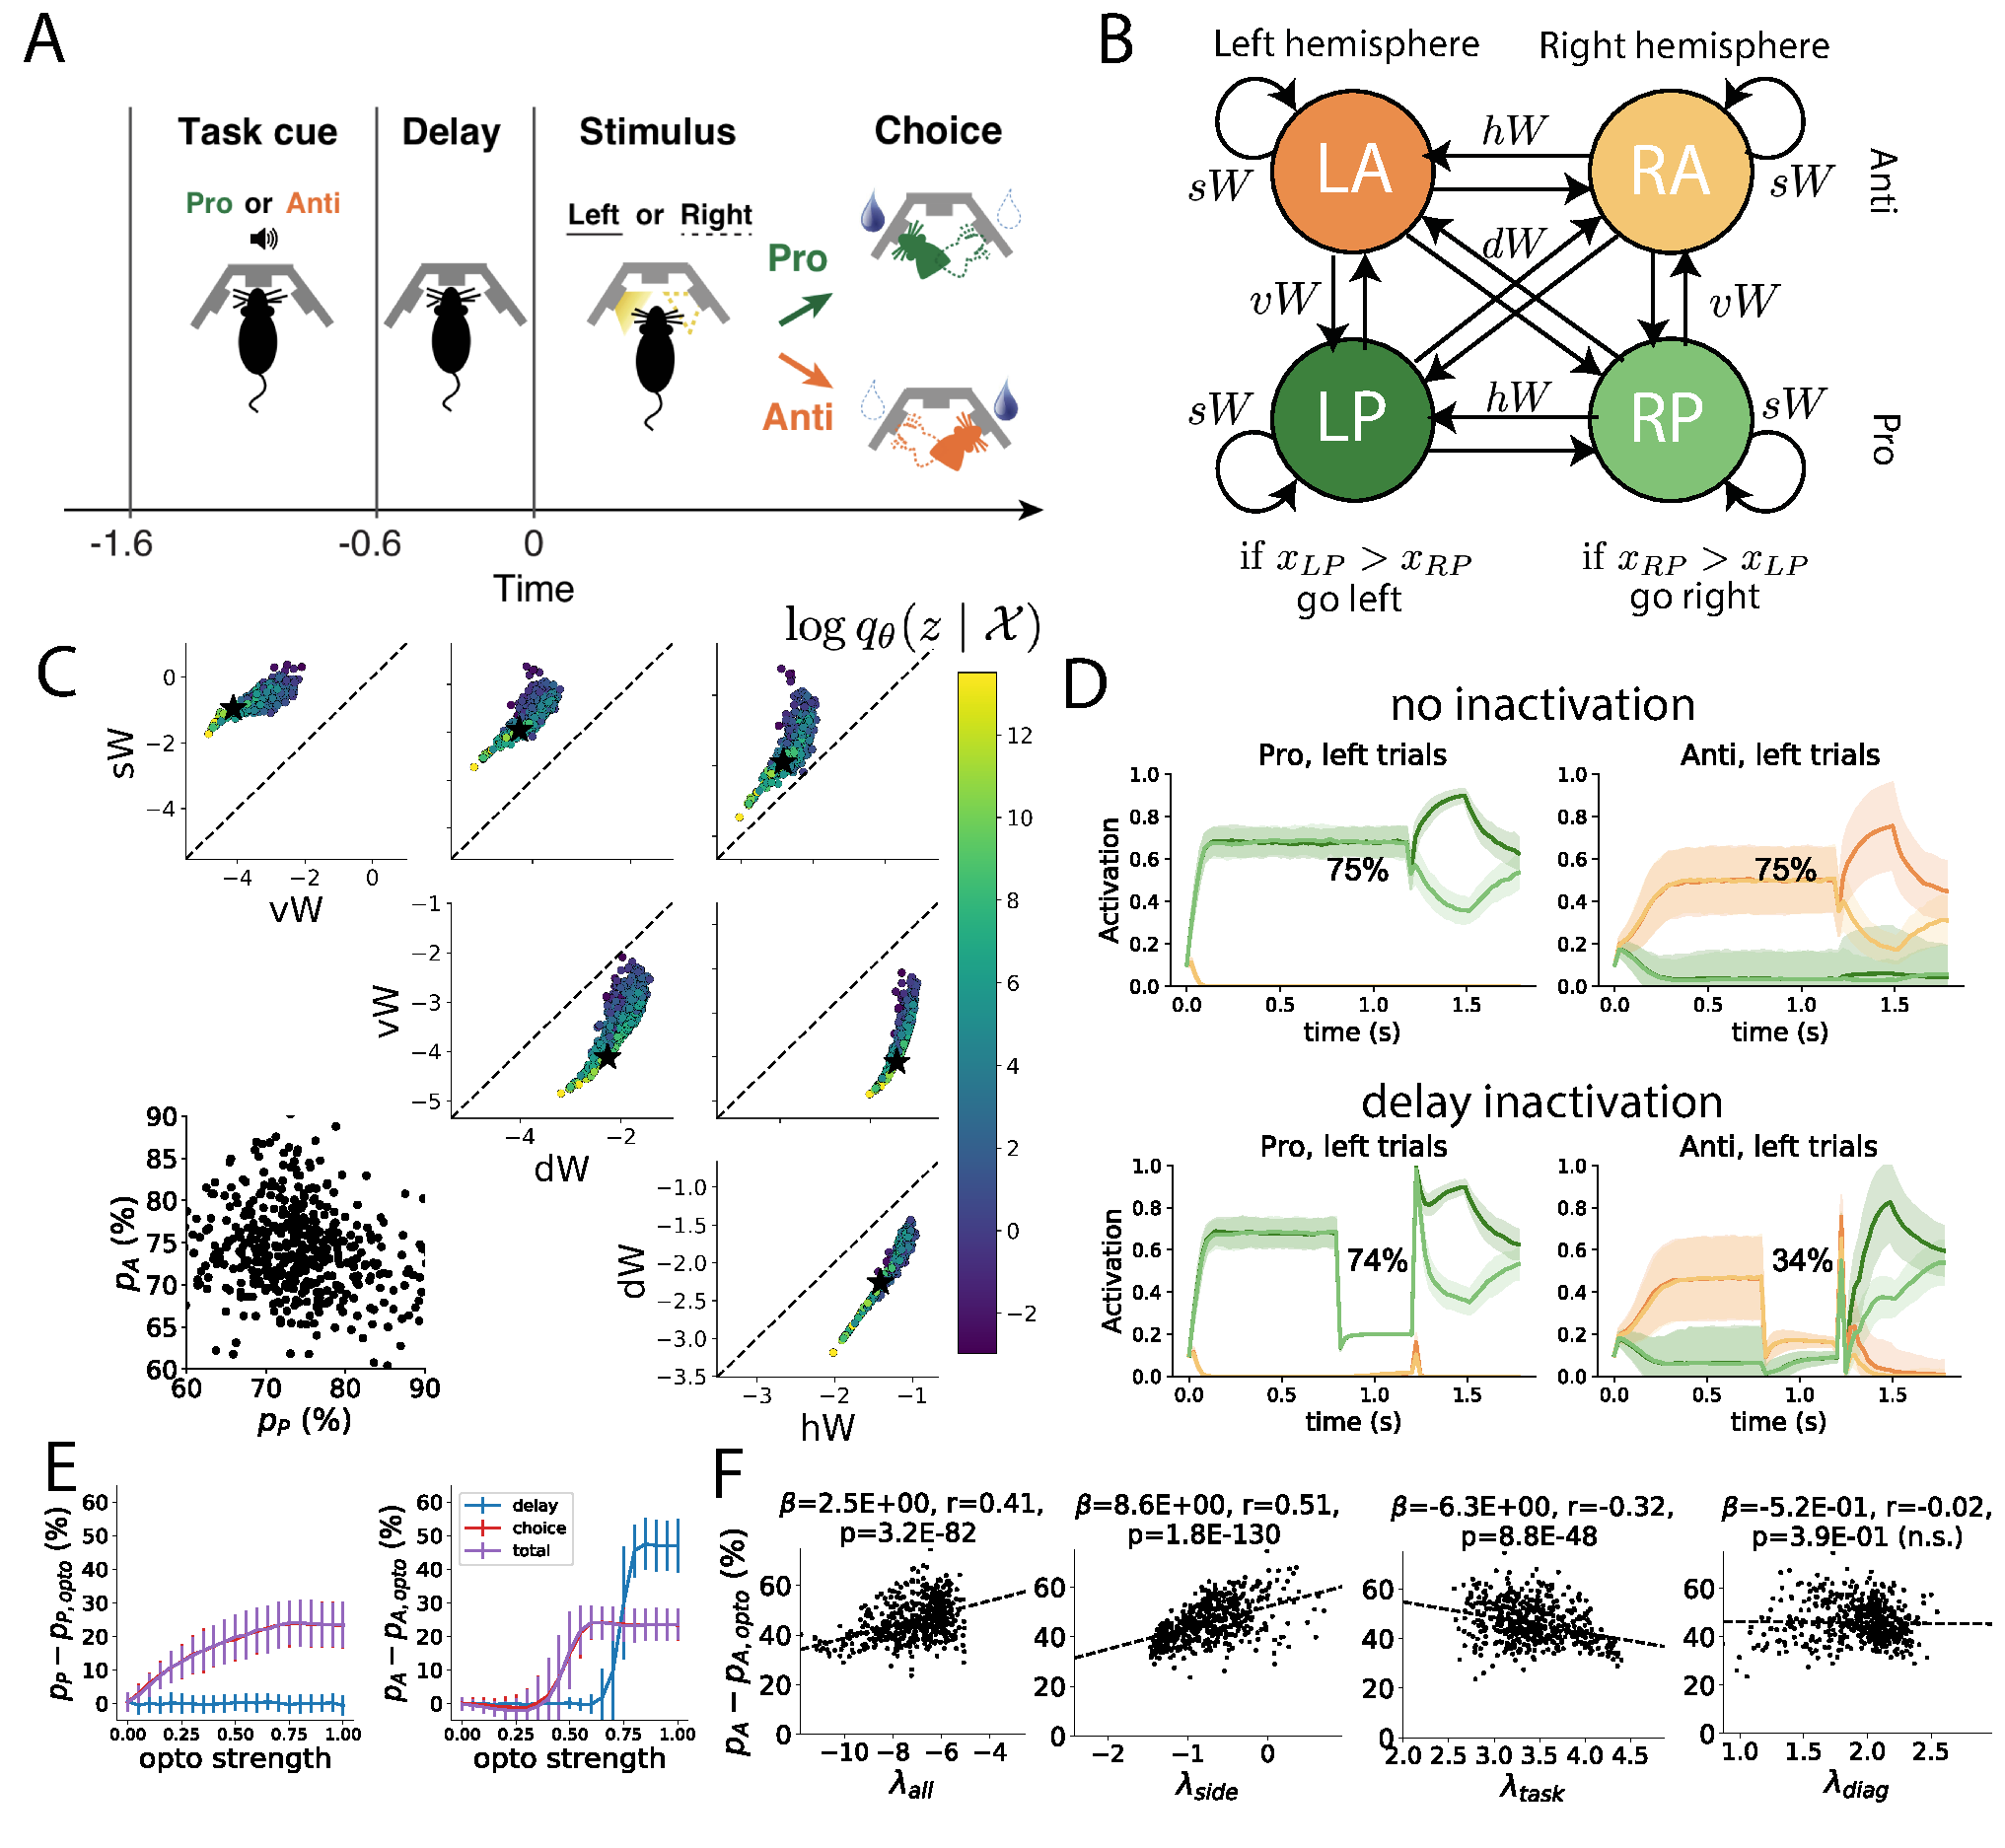
\includegraphics[scale=0.8]{figures/fig4/fig4.pdf}
\end{center}
\caption{\footnotesize 
\textbf{A}. Rapid task switching behavioral paradigm (see text). 
\textbf{B}. Model of superior colliculus (SC). Neurons: LP - left pro, RP - right pro, LA - left anti, RA - right anti. 
Parameters: $sW$ - self, $hW$ - horizontal, $vW$ -vertical, $dW$ - diagonal weights.  
\textbf{C}. The EPI inferred distribution of rapid task switching networks.  
Red and purple stars indicate modes $\mathbf{z}^*$ of each connectivity regime.
Sensitivity vectors $\mathbf{v}_1(\mathbf{z}^*)$ are shown by arrows.
(Bottom-left) EPI predictive distribution of task accuracies.
\textbf{D}. The connectivity regimes have different responses to perturbation.
(Top) Mean and standard error ($N_{\text{test}}$ = 25) of accuracy with respect to perturbation along the sensitivity dimension of each mode $\mathbf{z}^*$.
(Middle) Same with perturbation in the dimension of increasing $\lambda_{\text{task}}$ ($\mathbf{v}_{\text{task}}$).
(Bottom) Same with perturbation in the dimension of increasing $\lambda_{\text{diag}}$ ($\mathbf{v}_{\text{diag}}$).
}
\label{fig:SC}
\end{figure}

Rapid task switching is formalized mathematically as an emergent property with two statistics: accuracy in the Pro task $p_P(\mathbf{x}; \mathbf{z})$ and Anti task $p_A(\mathbf{x}; \mathbf{z})$.
We stipulate that accuracy be on average $.75$ in each task with variance $.075^2$
\begin{equation}\label{eq:SC_EP}
\begin{split}
\mathcal{X} ~~:~~ \mathbb{E}_{\mathbf{z}}\begin{bmatrix} p_P(\mathbf{x}; \mathbf{z}) \\ p_A(\mathbf{x}; \mathbf{z}) \end{bmatrix}  &~~=~~  \begin{bmatrix} .75 \\ .75 \end{bmatrix}  \\ 
 \text{Var}_{\mathbf{z}}\begin{bmatrix} p_P(\mathbf{x}; \mathbf{z}) \\ p_A(\mathbf{x}; \mathbf{z}) \end{bmatrix}  &~~=~~  \begin{bmatrix} .075^2 \\ .075^2  \end{bmatrix}.
\end{split}
\end{equation}
75\% accuracy is a realistic level of performance in each task, and with the chosen variance, inferred models will not exhibit fully random responses (50\%), nor perfect performance (100\%).

The EPI inferred distribution  (Fig. \ref{fig:SC}C) produces Pro and Anti task accuracies (Fig. \ref{fig:SC}C, middle-left) consistent with rapid task switching (Equation \ref{eq:SC_EP}).
This parameter distribution has intricate structure, that is not captured well by simple linear correlations (Fig. \ref{fig:SC1}).
Specifically, the shape of the EPI distribution changes dramatically on different sides of parameter space.
This is most saliently pointed out in the marginal distribution of  $sW$-$hW$ (Fig. \ref{fig:SC}C top-right), where anticorrelation between $sW$ and $hW$ switches to correlation with decreasing $sW$.
Not only has EPI captured this complicated distribution of connectivities producing rapid task switching, we can query the EPI distribution $q_{\bm{\theta}}(\mathbf{z} \mid \mathcal{X})$ to understand these two parametric regimes of SC connectivity.

To distinguish these two regimes, we use the EPI distribution to identify two sets of modes.
By fixing $hW$ to different values and doing gradient ascent on $\log q_{\bm{\theta}}(\mathbf{z} \mid \mathcal{X})$, we arrive at two solutions $\mathbf{z}^*(hW_{\text{fixed}}, r)$ where regime $r \in [1,2]$, and regime 1 is that of greater $sW$ (see Section \ref{methods_SC}).
As $hW_{\text{fixed}}$ increases, the modes coalesce to intermediate parameters reflecting a transition between the two sets of modes (Fig. \ref{fig:SC4} top).
By using EPI to connect these two regimes through this transitionary region of parameter space, we can explore what distinguishes the two regimes by stepping from the prototypical connectivity of regime 1 to that of regime 2.

While the connectivities gradually coalesce to the transitionary part of parameter space, the sensitivity dimensions $\mathbf{v}_1(\mathbf{z})$ are categorically different across regimes (Fig. \ref{fig:SC4} bottom).
The sensitivity dimension identifies the parameter combination which causes the emergent property to diminish with the shortest perturbation.
Since the two regimes have different $\mathbf{v}_1(\mathbf{z})$, this suggests they have different pathologies in their connectivity.
By perturbing connectivity in each regime along the sensitivity dimension, we can get a sense of the differing nature of these pathologies.

When perturbing connectivity along the sensitivity dimension, Pro accuracy monotonically increases in both regimes (Fig. \ref{fig:SC}D, top-left).
However, there is a stark difference between regimes in Anti accuracy. 
Anti accuracy falls in either direction of $\mathbf{v}_1$ in regime 1, yet monotonically increases along with Pro accuracy in regime 2 (Fig. \ref{fig:SC}D, top-right).
These distinct pathologies of rapid task switching are caused by distinct connectivity changes ($\mathbf{v}_1(\mathbf{z}^*(r=1))$ vs $\mathbf{v}_1(\mathbf{z}^*(r=2))$) and explain the sharp change in local structure of the EPI distribution.
With further perturbation analyses along dimensions of connectivity having established effects on processing, we are able to distinguish these two regimes with mechanistic insights (Fig. \ref{fig:SC}D, middle, bottom) (Section \ref{methods_SC}).

\subsection{EPI inferred SC connectivities reproduce results from optogenetic inactivation experiments} \label{results_SC_opt}

During the delay period of this task, the circuit must prepare to execute the correct task based on the cue input.
Experimental results from Duan et al. found that optogenetic inactivation of SC during the delay period consistently decreased performance in the Anti task, but had no effect on the Pro task (Fig. \ref{fig:SC_opto}A).
All network connectivities inferred by EPI exhibited this same effect, when network activities were silenced during the delay period (see Section \ref{methods_SC}).
Notably, EPI inferred connectivities were only conditioned upon the emergent property of rapid task switching, not on Anti task failure during delay period silencing.

Following delay period inactivation, there are strong similarities in the responses of Pro and Anti trials during the choice period (Fig. \ref{fig:SC5}A).
We interpreted these similarities to suggest that delay period inactivation flips the internal representation of task in the model.
Connectivity patterns inducing greater Pro task accuracy would antagonistically reduce accuracy in Anti trials subject to delay period inactivation in which this flip in task representation occurs.
In fact, across connectivities in the EPI inferred distribution, there was strong anti-correlation between Pro task accuracy $p_P$ and Anti task accuracy during delay period silencing $p_{A, opto}$ (Fig. \ref{fig:SC_opto}B).

We explored whether this antagonism between $p_P$ and $p_{A, opto}$ was present in each connectivity regime.
As in the previous section, we tested perturbations in the dimension of sensitivity $\mathbf{v}_1(\mathbf{z})$ from regime 1 to regime 2.
In both regimes, we recall that perturbations along $\mathbf{v}_1(\mathbf{z})$ yield increasing $p_P$.
We found that only in regime 2, does $p_{A,\text{opto}}$ decrease as $p_P$ increases(Fig. \ref{fig:SC_opto}C).
This context further distinguishes the two regimes discovered with EPI.

\begin{figure}
\begin{center}
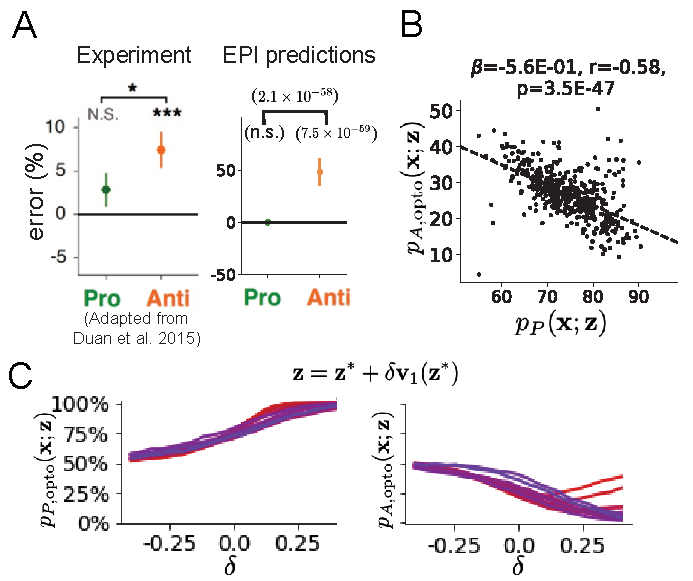
\includegraphics[scale=0.8]{figures/fig5/fig5.pdf}
\end{center}
\caption{\footnotesize 
\textbf{A}. The EPI distribution predicts experimental results (left) showing no change in the Pro task, but larger error in the Anti task (right).
\textbf{B}. Accuracy in the Anti task during delay period optogenetic inactivation $p_{A,\text{opto}}$ is strongly anticorrelated with accuracy in the Pro task.
\textbf{C}. Mean and standard error ($N_{\text{test}}$ = 25) of accuracy with respect to perturbation along the sensitivity dimension of each mode $\mathbf{z}^*$.
}
\label{fig:SC_opto}
\end{figure}

In summary, we used EPI to obtain the full distribution of connectivities that execute rapid task switching.
This EPI distribution revealed two regimes of rapid task switching, which we characterized using the probabilistic toolkit afforded by EPI.
We found that both of these parametric regimes identified by EPI reproduce results from optogenetic inactivation experiments: when activity is silenced during the delay period, only Anti accuracy suffers.
We then identified connectivity mechanisms governing Anti accuracy during delay period silencing, and showed the parametric regime they describe.

%To establish these two regimes of connectivity, we took gradient steps along $q_{\bm{\theta}}(\mathbf{z} \mid \mathcal{X})$ to produce modes $\mathbf{z}_1$ and $\mathbf{z}_2$  (Fig. \ref{fig:SC}C red and purple stars, Section \ref{methods_SC}).
%Simulations from these two regimes reveal different responses in each task (Fig. \ref{fig:SC}D).
%We charcaterized these regimes by identifying the dimensions of connectivity that rapid task switching is most sensitive to.
%The sensitivity dimensions $\mathbf{v}_1$ and  $\mathbf{v}_2$ (Fig. \ref{fig:SC}C, red and purple arrows) point in different directions, resulting in different changes to task accuracy (Fig. \ref{fig:SC}D, bottom-left, Fig. \ref{fig:SC2}).
%In regime 1, Anti accuracy diminishes in either direction of sensitivity away from the mode, while in regime 2, Anti accuracy matches monotonic increases in Pro accuracy.
%
%To understand why these distinct connectivity regimes have different failure modes, we can analyze the properties of connectivity in each regime.
%By taking the eigendecomposition of $W$, we can quantify how strongly different modes of processing are reflected in the connectivity matrix (see Section \ref{methods_SC}).  

%\subsection{Novel hypotheses from EPI} 
\section{Discussion} 
In neuroscience, machine learning has primarily been used to reveal structure in neural datasets \cite{paninski2018neural}.
Careful inference procedures are developed for these statistical models allowing precise, quantitative reasoning, which clarifies the way data informs beliefs about the model parameters.  
However, these statistical models often lack resemblance to the underlying biology, making it unclear how to go from the structure revealed by these methods, to the neural mechanisms giving rise to it. 
In contrast, theoretical neuroscience has focused on careful mechanistic modeling and the production of emergent properties of computation, rather than measuring structure in some noisy observed dataset.
%The careful steps of \emph{i}.) model design and \emph{ii}.) emergent property definition, are followed by \emph{iii}.) practical inference methods resulting in an opaque characterization of the way model parameters govern computation.  
In this work, we improve upon parameter inference techniques in theoretical neuroscience with emergent property inference, harnessing deep learning towards parameter inference with respect to emergent phenomena in  interpretable models of neural computation (see Section \ref{methods_related}).

Methodology for statistical inference in mechanistic models of neural circuits has evolved considerably in recent years.
Early work used rejection sampling techniques \cite{beaumont2002approximate, marjoram2003markov,sisson2007sequential}, but more recently developed methodology employs deep learning to improve efficiency or provide flexible distribution approximations.
SNPE \cite{gonccalves2019training} and other sequential techniques for inference in mechanistic models developed along with EPI (see Section \ref{methods_related}) have been used for posterior inference with noisy experimental datasets.
On the other hand, EPI is a deep inference technique designed to condition directly on emergent properties, such that the parameter distribution only produces the computation of interest.
EPI is thus ideally suited for questions in theoretical neuroscience, and we show that it has superior scaling properties to these other inference techniques (see Section \ref{results_LRRNN}).


%In neuroscience, machine learning has primarily been used to reveal structure in neural datasets \cite{paninski2018neural}.
%Careful inference procedures are developed for these statistical models allowing precise, quantitative reasoning, which clarifies the way data informs beliefs about the model parameters.  
%However, these statistical models often lack resemblance to the underlying biology, making it unclear how to go from the structure revealed by these methods, to the neural mechanisms giving rise to it. 
%In contrast, theoretical neuroscience has focused on careful mechanistic modeling and the production of emergent properties of computation.  
%The careful steps of \emph{i}.) model design and \emph{ii}.) emergent property definition, are followed by \emph{iii}.) practical inference methods resulting in an opaque characterization of the way model parameters govern computation.  
%In this work, we improve upon parameter inference techniques in theoretical neuroscience with emergent property inference, harnessing deep learning towards careful inference in careful models of neural computation (see Section \ref{methods_related}).
%
%Specifically, approximate Bayesian computation \cite{beaumont2002approximate, marjoram2003markov, sisson2007sequential} has been the standard approach to parameter inference in neural circuit models lacking tractable likelihoods.
%ABC methods do not confer probabilities on accepted parameters, require an acceptance threshold chosen to trade-off inference quality with tractability, do not scale efficiently to high-dimensional parameter spaces, and require independent techniques to analyze sensitivity for local parameter choices \cite{sisson2018handbook}.
%In contrast, EPI allows probability evaluations at any point in parameter space, conditions distributions on the natural quantification of emergent properties, scales to high dimensional parameter spaces, and admits fast sensitivity calculations.
%
%Technically, EPI is a maximum entropy method, which learns parameter distributions that are as random as possible given that they produce the emergent property.
%Conceptually, maximally random distributions given some constraints are useful for understanding parametric sensitivity.
%This is well understood in Bayesian inference, where maximum entropy is the chosen normative principle.
%This is emphasized by an innovative formalism unifying top-down maximum entropy normative models with bottom-up statistical models \cite{mlynarski2020statistical}.
%Indeed, EPI is an adaptive variational inference program, and may be considered to have a Bayesian uniform prior (see Section \ref{methods_VI}).
%
%Biologically realistic models of neural circuits often prove formidable to analyze for two main reasons.
%A primary challenge is that the number of parameters scales dramatically with the number of neurons, limiting analysis of its parameter space.
%We see in Section \ref{results_LRRNN} that EPI scales seamlessly to high dimensional parameter spaces of RNN connectivities, while maintaining the production of the specified emergent property.
%EPI strongly outperforms the standard likelihood-free inference technique (SMC-ABC \cite{sisson2007sequential}), and a recently developed deep likelihood-free inference technique (SNPE \cite{gonccalves2019training}), most likely because of it's ability to leverage the gradient information of the emergent property statistics and to adapt it's paramter sampling distribution at every step of gradient descent.
%
%A secondary challenge is that the structure of the parametric regimes governing emergent properties is intricate.  
%For example, even in low dimensional circuits, models can support more than one steady state \cite{kraynyukova2018stabilized} and non-trivial dynamics on strange attractors \cite{morrison2016diversity}.
%With EPI, we use deep probabillity distributions to capture the complex nonlinear parameter distributions governing model behavior.
%In Section \ref{results_V1}, we used EPI to reveal a curved parametric manifolds governing curcuit variability in the stochastic stabilized supralinear network, and used hypothesis testing techniques to validate our findings.
%In Section \ref{results_SC}, we identified two regimes of SC connectivity resulting in rapid task switching, and found that the full distribution of rapid task switching networks reproduced an experimental result.
%
%EPI leverages deep learning technology for neuroscientific inquiry in a categorically different way than approaches focused on training neural networks to execute behavioral tasks \cite{richards2019deep}. 
%These works focus on examining optimized deep neural networks while considering the objective function, learning rule, and architecture used.
%This endeavor efficiently obtains sets of parameters that can be reasoned about with respect to such considerations, but lacks the careful probabilistic treatment of parameter inference in EPI.
%All of these approaches can be used complementarily to enhance the practice of theoretical neuroscience.


\textbf{Acknowledgements}: \\
This work was funded by NSF Graduate Research Fellowship,  DGE-1644869, McKnight Endowment Fund, NIH NINDS 5R01NS100066, Simons Foundation 542963, NSF NeuroNex Award, DBI-1707398, The Gatsby Charitable Foundation, Simons Collaboration on the Global Brain Postdoctoral Fellowship, Chinese Postdoctoral Science Foundation, and International Exchange Program Fellowship. 
Helpful conversations were had with Francesca Mastrogiuseppe, Srdjan Ostojic, James Fitzgerald, Stephen Baccus, Dhruva Raman, Liam Paninski, and Larry Abbott.

\textbf{Data availability statement}: \\
The datasets generated during and/or analyzed during the current study are available from the corresponding author upon reasonable request.

\textbf{Code availability statement}: \\
All software written for the current study is available at https://github.com/cunningham-lab/epi.

\bibliography{eLife2020}
\bibliographystyle{unsrt}

\newpage 

\section{Methods}

\subsection{Emergent property inference (EPI)}\label{methods_EPI}
%Consider model parameterization $\mathbf{z}$ and data $\mathbf{x}$ which has an intractable likelihood $p(\mathbf{x} \mid \mathbf{z})$ defined by a model simulator of which samples are available $\mathbf{x} \sim p(\mathbf{x} \mid \mathbf{z})$.  
%EPI optimizes a distribution $q_{\bm{\theta}}(\mathbf{z})$ (itself parameterized by $\bm{\theta}$) of model parameters $\mathbf{z}$ to produce an emergent property of interest $\mathcal{X}$ defined by the means and variances of emergent property statistics $f(\mathbf{x}; \mathbf{z})$
% \begin{equation}
%\mathcal{X}: \mathbb{E}_{\mathbf{z},\mathbf{x}}\left[f(\mathbf{x}; \mathbf{z})\right] = \bm{\mu}, \text{Var}_{\mathbf{z},\mathbf{x}}\left[f(\mathbf{x}; \mathbf{z})\right] = \bm{\sigma}^2.
%\end{equation}
%Precisely, the emergent property statistics $f(\mathbf{x})$ must have means $\bm{\mu}$ and variances $\bm{\sigma}^2$  over the EPI distribution of parameters $q_{\bm{\theta}}(\mathbf{z})$ and stochasticity of the data given the parameters defined by the model $p(\mathbf{x} \mid \mathbf{z})$.  
%This is a viable way to represent emergent properties in theoretical models, as we have demonstrated in the main text, and enables the EPI optimization.
%
%
%With EPI, we use deep probability distributions to learn flexible approximations to model parameter distributions $q_{\bm{\theta}}(\mathbf{z})$.
% In deep probability distributions, a simple random variable $\mathbf{z}_0 \sim q_0(\mathbf{z}_0)$ is mapped deterministically via a sequence of deep neural network layers ($g_1$, .. $g_l$) parameterized by weights and biases $\bm{\theta}$ to the support of the distribution of interest:
%\begin{equation}
%\mathbf{z} = g_{\bm{\theta}}(\mathbf{z}_0) = g_l(..g_1(\mathbf{z}_0)) \sim q_{\bm{\theta}}(\mathbf{z}).
%\end{equation}
%Given a simulator defined by a theoretical model $\mathbf{x} \sim p(\mathbf{x} \mid \mathbf{z})$ and some emergent property of interest $\mathcal{X}$, $q_{\bm{\theta}}(\mathbf{z})$ is optimized via the neural network parameters $\bm{\theta}$ to find a maximally entropic distribution $q_{\bm{\theta}}^*$ within the deep variational family $\mathcal{Q}$ producing the emergent property:
%\begin{equation} \label{eq:opt}
%\begin{split}
%q_{\bm{\theta}}^*(\mathbf{z}) &= \argmax_{q_{\bm{\theta}} \in Q} H(q_{\bm{\theta}}(\mathbf{z})) \\
% &  \text{s.t.  } \mathbb{E}_{\mathbf{z},\mathbf{x}}\left[f(\mathbf{x}; \mathbf{z})\right] = \bm{\mu}, \text{Var}_{\mathbf{z},\mathbf{x}}\left[f(\mathbf{x}; \mathbf{z})\right] = \bm{\sigma}^2. \\
% \end{split}
%\end{equation} 
%Since we are optimizing parameters $\bm{\theta}$ of our deep probability distribution with respect to the entropy $H(q_{\bm{\theta}}(\mathbf{z}))$, we must take gradients with respect to the log probability density of samples from the deep probability distribution.  
%Entropy of $q_{\bm{\theta}}(\mathbf{z})$ can be expressed as an expectation of the negative log density of parameter samples $\mathbf{z}$ over the randomness in the parameterless initial distribution $q_0$:
%\begin{equation}
%H(q_{\bm{\theta}}(\mathbf{z})) = \int - q_{\bm{\theta}}(\mathbf{z}) \log(q_{\bm{\theta}}(\mathbf{z})) d\mathbf{z} = \mathbb{E}_{\mathbf{z} \sim q_{\bm{\theta}}}\left[-\log(q_{\bm{\theta}}(\mathbf{z})) \right] = \mathbb{E}_{\mathbf{z}_0 \sim q_0}\left[-\log(q_{\bm{\theta}}(g_{\bm{\theta}}(\mathbf{z}_0))) \right].
%\end{equation}
%Thus, the gradient of the entropy of the deep probability distribution can be estimated as an average of gradients of the log density of samples $\mathbf{z}$:
%\begin{equation}
%\nabla_{\bm{\theta}} H(q_{\bm{\theta}}(\mathbf{z})) = \mathbb{E}_{\mathbf{z}_0 \sim q_0}\left[- \nabla_{\bm{\theta}} \log(q_{\bm{\theta}}(g_{\bm{\theta}}(\mathbf{z}_0))) \right].
%\end{equation}
%In EPI, MEFNs are purposed towards variational learning of model parameter distributions.

Determining the combinations of model parameters that can produce observed data or a desired output is a key part of scientific practice.
Solving inverse problems is especially important in neuroscience, since we require complex models to describe the complex phenomena of neural computations.
While much machine learning research has focused on how to find latent structure in large-scale neural datasets, less has focused on inverting theoretical circuit models conditioned upon the emergent phenomena they produce.
Here, we introduce a novel method for statistical inference, which finds distributions of parameter solutions that only produce the desired emergent property.
This method seamlessly handles neural circuit models with stochastic nonlinear dynamical generative processes, which are predominant in theoretical neuroscience.

 
Consider model parameterization $\mathbf{z}$, which is a collection of scientifically interesting variables that govern the complex simulation of data $\mathbf{x}$.
For example (see Section \ref{results_motivating}), $\mathbf{z}$ may be the electrical conductance parameters of an STG subcircuit, and $\mathbf{x}$ the evolving membrane potentials of the five neurons.
In terms of statistical modeling, this circuit model has an intractable likelihood $p(\mathbf{x} \mid \mathbf{z})$, which is predicated by the stochastic differential equations that define the model.
Even so, we do not scientifically reason about how $\mathbf{z}$ governs all of $\mathbf{x}$, but rather specific phenomena that are a function of the data $f(\mathbf{x}; \mathbf{z})$.
In the STG example, $f(\mathbf{x}; \mathbf{z})$ measures hub neuron frequency from the evolution of $\mathbf{x}$ governed by $\mathbf{z}$.
With EPI, we learn distributions of $\mathbf{z}$ that results in an average and variance of $f(\mathbf{x}; \mathbf{z})$, denoted $\bm{\mu}$ and $\bm{\sigma}^2$.
We refer to the collection of these statistical moments as an emergent property.
Such emergent properties $\mathcal{X}$ are defined through choice of $f(\mathbf{x}; \mathbf{z})$ (which may be one or multiple statistics), $\bm{\mu}$, and $\bm{\sigma}^2$
 \begin{equation}
\mathcal{X}: \mathbb{E}_{\mathbf{z},\mathbf{x}}\left[f(\mathbf{x}; \mathbf{z})\right] = \bm{\mu}, \text{Var}_{\mathbf{z},\mathbf{x}}\left[f(\mathbf{x}; \mathbf{z})\right] = \bm{\sigma}^2.
\end{equation}
Precisely, the emergent property statistics $f(\mathbf{x}; \mathbf{z})$ must have means $\bm{\mu}$ and variances $\bm{\sigma}^2$  over the EPI distribution of parameters and stochasticity of the data given the parameters.
By defining these means and variances over both levels of stochasticity -- the inferred distribution and that of the model -- there is a fine degree of control over predictions made by the inferred parameters.

In EPI, deep probability distributions are optimized to learn the inferred distribution.
 In deep probability distributions, a simple random variable $\mathbf{z}_0 \sim q_0(\mathbf{z}_0)$ is mapped deterministically via a sequence of deep neural network layers ($g_1$, .. $g_l$) parameterized by weights and biases $\bm{\theta}$ to the support of the distribution of interest:
\begin{equation}
\label{eq:deep_transform}
\mathbf{z} = g_{\bm{\theta}}(\mathbf{z}_0) = g_l(..g_1(\mathbf{z}_0)) \sim q_{\bm{\theta}}(\mathbf{z}).
\end{equation}
Such deep probability distributions embed the inferred distribution in a deep network.
Once optimized, this deep network representation has remarkably useful properties: fast sampling, probability evaluations, and also first- and second-order probability gradient evaluations.

By choosing a neural circuit model, often represented as a system of differential equations, we implictly definge a model likelihood $p(\mathbf{x} \mid \mathbf{z})$, which may be unknown or intractable for our purposes.  Given this model choice and that of an emergent property $\mathcal{X}$, $q_{\bm{\theta}}(\mathbf{z})$ is optimized via the neural network parameters $\bm{\theta}$ to find a maximally entropic distribution $q_{\bm{\theta}}^*$ within the deep variational family $\mathcal{Q}$ producing the emergent property $\mathcal{X}$:
\begin{equation} \label{eq:opt}
\begin{split}
q_{\bm{\theta}}(\mathbf{z} \mid \mathcal{X}) = q_{\bm{\theta}}^*(\mathbf{z}) &= \argmax_{q_{\bm{\theta}} \in Q} H(q_{\bm{\theta}}(\mathbf{z})) \\
 &  \text{s.t.  } \mathcal{X} ~~:~~ \mathbb{E}_{\mathbf{z},\mathbf{x}}\left[f(\mathbf{x}; \mathbf{z})\right] = \bm{\mu}, \text{Var}_{\mathbf{z},\mathbf{x}}\left[f(\mathbf{x}; \mathbf{z})\right] = \bm{\sigma}^2. \\
 \end{split}
\end{equation} 
Entropy is chosen as the normative selection principle to match that of Bayesian inference (see Section \ref{methods_ME_EF}).
However, a key difference is that variational inference and other Bayesian methods do not constrain the predictions of their inferred parameter distribution.
This optimization is executed using the algorithm of Maximum Entropy Flow Networks (MEFNs) \cite{loaiza2017maximum}.


In the remainder of Section \ref{methods_EPI}, we will explain the finer details and motivation of the EPI method. 
First, we explain related approaches and what EPI introduces to this domain (Section \ref{methods_related}).
Second, we describe the special class of deep probability distributions used in EPI called normalizing flows (Section \ref{methods_NF}).  
Next, we explain the constrained optimization technique used to solve Equation \ref{eq:opt} (Section \ref{methods_AL_opt}).
Then, we demonstrate the details of this optimization in a toy example (Section \ref{methods_2DLDS}).
Finally, we establish the known relationship between maximum entropy distributions and exponential families (Section \ref{methods_ME_EF}), which is used to explain how EPI can be viewed as a form of variational inference (Section \ref{methods_VI}).

 \subsubsection{Related approaches}\label{methods_related}
 When Bayesian inference problems lack conjugacy, scientists use approximate inference methods like variational inference (VI) \cite{saul1998mean} and Markov chain Monte Carlo (MCMC) \cite{metropolis1953equation, hastings1970monte}. 
After optimization, variational methods return a parameterized posterior distribution, which we can analyze.
Also, the variational approximating distribution class is often chosen such that it permits fast sampling.
In contrast MCMC methods only produce samples from the approximated posterior distribution.
No parameterized distribution is estimated, and additional samples are always generated with the same sampling complexity.
Inference in models defined by systems of differential has been demonstrated with MCMC \cite{girolami2011riemann}, although this approach requires tractable likelihoods.
Advancements have leveraged structure in stochastic differential equation models to improve likelihood approximations, thus expanding the domain of applicable models \cite{golightly2011bayesian}.
 
Simulation-based inference \cite{cranmer2020frontier} is model parameter inference in the absence of a tractable likelihood function.
The most prevalent approach to simulation-based inference is approximate Bayesian computation \cite{beaumont2002approximate}, in which satisfactory parameter samples are kept from random prior sampling according to a rejection heuristic.
The obtained set of parameters do not have a probabilities, and further insight about the model must be gained from examination of the parameter set and their generated activity.
Methodological advances to ABC methods have come through the use of Markov chain Monte Carlo (MCMC-ABC) \cite{marjoram2003markov} and sequential Monte Carlo (SMC-ABC) \cite{sisson2007sequential} sampling techniques.
SMC-ABC is considered state-of-the-art ABC, yet this approach still struggles to scale in dimensionality (cf. Fig. \ref{fig:LRRNN}).
Furthermore, once a parameter set has been obtained by SMC-ABC from a finite set of particles, the SMC-ABC algorithm must be run again from scratch with a new population of initialized particles to obtain additional samples.

For scientific model analysis, we seek a parameter distribution exhibiting the properties of a well-chosen variational approximation: a parametric form conferring analytic calculations, and trivial sampling time.
For this reason, ABC and MCMC techniques are unattractive, since they only produce a set of parameter samples and have unchanging sampling rate.
EPI infers parameters in mechanistic models using the MEFN \cite{loaiza2017maximum} algorithm using a deep variational approximation.
The deep neural network of EPI defines the parametric form of the distribution approximation.
Furthermore, the EPI distribution is constrained to produce an emergent property.
In other words, the summary statistics of the posterior predictive distribution are fixed to have certain first and second moments.
EPI optimization is enabled using stochastic gradient techniques in the spirit of likelihood-free variational inference \cite{tran2017hierarchical}.
The analytic relationship between EPI and variational inference is explained in Secton \ref{methods_VI}.

 We note that, during our preparation and early presentation of this work \cite{bittner2019degenerate, bittner2019examining}, another work has arisen with broadly similar goals: bringing statistical inference to mechanistic models of neural circuits (\cite{nonnenmacher2018sbi, desitler2019statistical, gonccalves2019training}).%, preprint posted simultaneously with this preprint).
We are encouraged by this general problem being recognized by others in the community, and we emphasize that these works offer complementary neuroscientific contributions (different theoretical models of focus) and use different technical methodologies (ours is built on our prior work \cite{loaiza2017maximum}, theirs similarly \cite{LueckmannGoncalves_17}).

The method EPI differs from SNPE in some key ways.
SNPE belongs to a ``sequential" class of recently developed simulation-based inference methods in which two neural networks are used for posterior inference.
This first neural network is a deep probability distribution (normalizing flow) used to estimate the posterior $p(\mathbf{z} \mid \mathbf{x})$ (SNPE) or the likelihood  $p(\mathbf{x} \mid \mathbf{z})$ (sequential neural likelihood (SNL \cite{papamakarios2019sequential})).
A recent advance uses an unconstrained neural network to estimate the likelihood ratio (sequential neural ratio estimation (SNRE \cite{hermans2020likelihood}).
In SNL and SNRE, MCMC sampling techniques are used to obtain samples from the approximated posterior.
This contrasts with EPI and SNPE, which use deep probability distributions to model parameters, which facilitates immediate measurements of sample probability, gradient, or Hessian for system analysis.
The second neural network in this sequential class of methods is the amortizer.  This unconstrained deep network maps data $\mathbf{x}$ (or statistics $f(\mathbf{x}; \mathbf{z})$ or model parameters $\mathbf{z}$ to the weights and biases of the first neural network.
These methods are optimized on a conditional density (or ratio) estimation objective.
The data used to optimize this objective are generated via an adaptive procedure, in which training data pairs ($\mathbf{x}_i$, $\mathbf{z}_i$) become sequentiall closer to the true data and posterior.

The approximating fidelity of the deep probability distribution in sequential approaches is optimized to generalize across the training distribution of the conditioning variable.
This generalization property of the sequential methods can reduce the accuracy at the singular posterior of interest.
Whereas in EPI, the entire expressivity of the deep probability distribution is dedicated to learning a single distribution as well as possible.
Amortization is not possible in EPI, since EPI learns an exponential family distribution parameterized by its mean (see Section \ref{methods_ME_EF}).
Since EPI distributions are defined by the mean $\bm{\mu}$ of their statistics, there is the well-known inverse mapping problem of exponential families \cite{wainwright2008graphical} that prohibits an amortization based approach.
However, we have shown that the same two-network architecture of the sequential simulation-based inference methods can be used for amortized inference in intractable exponential family posteriors using their natural parameterization \cite{bittner2019approximating}.

Finally, one important differentiating factor between EPI and sequential simulation-based inference methods is that EPI leverages gradients $\nabla_{\mathbf{z}} f(\mathbf{x}; \mathbf{z})$ during optimization.
These gradients can improve convergence time and scalability, as we have shown on an example conditioning low-rank RNN connectivity on the property of stable amplification (see Section \ref{results_LRRNN}).
With EPI, we prove out the suggestion that a deep inference technique can improve efficiency by leveraging these model gradients when they are tractable.
Sequential simulation-based inference techniques may be better suited for sceintific problems where $\nabla_{\mathbf{z}} f(\mathbf{x}; \mathbf{z})$ is intractable or unavailable: when there is a nondifferentiable model or it requires lengthy simulations.
However, the sequential simulation-based inference techniques cannot constrain the predictions of the inferred distribution in the manner of EPI.

Structural identifiability analysis involves the measurement of sensitivity and unidentifiabilities in natural models.
Around a point, one can measure the Jacobian. One approach that scales well is EAR \cite{karlsson2012efficient}.
A popular efficient approach for systems of ODEs has been neural ODE adjoint \cite{chen2018neural} and its stochastic adaptation \cite{li2020scalable}.
Casting identifiability as a statistical estimation problem, the profile likelihood can assess via iterated optimization while holding parameters fixed \cite{raue2009structural}.
An exciting recent method is capable of recovering the functional form of such unidentifiabilities away from a point by following degenerate dimensions of the fisher information matrix \cite{raman2017delineating}.
Global structural non-identifiabilities can be found for models with polynomial or rational dynamics equations using DAISY \cite{saccomani2003parameter}.
With EPI, we have all the benefits given by a statistical inference method plus the ability to query the first- or second-order gradient of the probability of the inferred distribution at any chosen parameter value.
The second-order gradient of the log probability (the Hessian), which is directly afforded by EPI distributions, produces salient information about parametric sensitivty of the emergent property.
For example, the eigenvector with most negative eigenvalue of the Hessian shows parametric combinations away from a parameter choice that decrease the in EPI distribution probability the fastest.
We refer to this eigenvector as the sensitivity dimension, and it is used to generate scientific insight about a model of superior colliculus connectivity (see Section \ref{results_SC}). 

%\cite{dhruva/goldman papers}

%A closely related methodology, variational inference, uses optimization to approximate posterior distributions \cite{blei2017variational}.
%Standard methods like stochastic gradient variational Bayes \cite{kingma2013auto} or black box variational inference \cite{ranganath2014black} simply do not work for inference in theoretical models of neural circuits, since they require tractable likelihoods $p(\mathbf{x} \mid \mathbf{z})$.
%Work on likelihood-free variational inference (LFVI) \cite{tran2017hierarchical}, which like EPI seeks to do inference in models with intractable likelihoods, employs an additional deep neural network as a ratio estimator, enabling an estimation of the optimization objective for variational inference.
%Like LFVI, EPI can be framed as variational inference (see Section \ref{methods_VI}).
%But, unlike LFVI, EPI uses a single deep network to learn a distribution and is optimized to produce an emergent property, rather than condition on data points.  
%Optimizing the EPI objective is a technological challenge, the details of which we elaborate in Section \ref{methods_AL_opt}.  
%Before going through those details, we ground this optimization in a toy example.
% We note that, during our preparation and early presentation of this work \cite{bittner2019degenerate, bittner2019examining}, another work has arisen with broadly similar goals: bringing statistical inference to mechanistic models of neural circuits (\cite{nonnenmacher2018sbi, desitler2019statistical, gonccalves2019training}, preprint posted simultaneously with this preprint).
%We are encouraged by this general problem being recognized by others in the community, and we emphasize that these works offer complementary neuroscientific contributions (different theoretical models of focus) and use different technical methodologies (ours is built on our prior work \cite{loaiza2017maximum}, theirs similarly \cite{LueckmannGoncalves_17}).
%These distinct methodologies and scientific investigations emphasize the increased importance and timeliness of both works. 

\subsubsection{Deep probability distributions and normalizing flows}\label{methods_NF}
Deep probability distributions are comprised of multiple layers of fully connected neural networks (Equation \ref{eq:deep_transform}).
When each neural network layer is restricted to be a bijective function, the sample density can be calculated using the change of variables formula at each layer of the network.  For $\mathbf{z}_i = g_i(\mathbf{z_{i-1}})$,
%\begin{equation}
%q(\mathbf{z}') = q(f^{-1}(\mathbf{z}')) \left| \det \frac{\partial f^{-1}(\mathbf{z}')}{\partial \mathbf{z}'} \right| = q(\mathbf{z}) \left| \det \frac{\partial f(\mathbf{z})}{\partial \mathbf{z}} \right|^{-1}.
%\end{equation}
\begin{equation}
p(\mathbf{z}_i) = p(g_i^{-1}(\mathbf{z}_i)) \left| \det \frac{\partial g_i^{-1}(\mathbf{z}_i)}{\partial \mathbf{z}_i} \right| = p(\mathbf{z}_{i-1}) \left| \det \frac{\partial g_i(\mathbf{z}_{i-1})}{\partial \mathbf{z}_{i-1}} \right|^{-1}.
\end{equation}

However, this computation has cubic complexity in dimensionality for fully connected layers.  
By restricting our layers to normalizing flows \cite{rezende2015variational, papamakarios2019normalizing} -- bijective functions with fast log determinant Jacobian computations, which confer a fast calculation of the sample log probability.
Fast log probability calculation confers efficient optimization of the maximum entropy objective (see Section \ref{methods_AL_opt}).
%Most of our analyses use either a planar flow \cite{rezende2015variational} or real NVP \cite{dinh2017density}, which have proven effective in our architecture searches.  
%Planar flow architectures are specified by the number of planar bijection layers used, while real NVP architectures are specified by the number of masks, neural network layers per mask, units per layer, and batch normalization momentum parameter.
We use the Real NVP \cite{dinh2017density} normalizing flow class, because its coupling architecture confers both fast sampling (forward) and fast log probability evaluation (backward).
Fast probability evaluation in turn facilitates fast gradient and Hessian evaluation of log probability throughout parameter space.
Glow permutations were used in between coupling stages \cite{kingma2018glow}.
This is in contrast to autoregressive architectures \cite{papamakarios2017masked, kingma2016improved}, in which only one of the forward or backward passes can be efficient.
In this work, normalizing flows are used as flexible posterior approximations $q_{\bm{\theta}}(\mathbf{z})$ having weights and biases $\bm{\theta}$. 
We specify the architecture used in each application by the number of Real-NVP affine coupling stages, and the number of neural network layers and units per layer of the conditioning functions.

\subsubsection{Augmented Lagrangian optimization}\label{methods_AL_opt}
To optimize $q_{\bm{\theta}}(\mathbf{z})$ in Equation \ref{eq:opt}, the constrained maximum entropy optimization is executed using the augmented Lagrangian method.  
The following objective is minimized:
\begin{equation} \label{eq:AL}
L(\bm{\theta}; \bm{\eta}_{\text{opt}}, c) = -H(q_{\bm{\theta}}) + \bm{\eta}_{\text{opt}}^\top R(\bm{\theta}) + \frac{c}{2}||R(\bm{\theta})||^2
\end{equation}
where average constraint violations $R(\bm{\theta}) = \mathbb{E}_{\mathbf{z} \sim q_{\bm{\theta}}}\left[ \mathbb{E}_{\mathbf{x}\sim p(\mathbf{x} \mid \mathbf{z})}\left[T(\mathbf{x}; \mathbf{z}) - \bm{\mu}_{\text{opt}} \right] \right]$, $\bm{\eta}_{\text{opt}} \in \mathbb{R}^m$ are the Lagrange multipliers where $m = |\bm{\mu}_{\text{opt}}| = |T(\mathbf{x}; \mathbf{z})| = 2|f(\mathbf{x}; \mathbf{z})|$,  and $c$ is the penalty coefficient. 
The sufficient statistics $T(\mathbf{x}; \mathbf{z})$ and mean parameter $\bm{\mu}_{\text{opt}}$ are determined by the means $\bm{\mu}$ and variances $\bm{\sigma}^2$ of emergent property statistics $f(\mathbf{x}; \mathbf{z})$ defined in Equation \ref{eq:opt} (see Section \ref{methods_VI}).
Specifically, $T(\mathbf{x}; \mathbf{z})$ is a concatenation of the first and second moments, $\bm{\mu}_{\text{opt}}$ is a concatenation of $\bm{\mu}$ and $\bm{\sigma}^2$ (see section \ref{methods_ME_EF}), and the Lagrange multipliers are closely related to the natural parameters $\bm{\eta}$ of exponential families (see Section \ref{methods_ME_EF}).
Weights and biases $\bm{\theta}$ of the deep probability distribution are optimized according to Equation \ref{eq:AL} using the Adam optimizer with learning rate $10^{-3}$ \cite{kingma2014adam}.

The gradient with respect to entropy $H(q_{\bm{\theta}}(\mathbf{z}))$ can be expressed using the reparameterization trick as an expectation of the negative log density of parameter samples $\mathbf{z}$ over the randomness in the parameterless initial distribution $q_0(\mathbf{z}_0$):
\begin{equation}
H(q_{\bm{\theta}}(\mathbf{z})) = \int - q_{\bm{\theta}}(\mathbf{z}) \log(q_{\bm{\theta}}(\mathbf{z})) d\mathbf{z} = \mathbb{E}_{\mathbf{z} \sim q_{\bm{\theta}}}\left[-\log(q_{\bm{\theta}}(\mathbf{z})) \right] = \mathbb{E}_{\mathbf{z}_0 \sim q_0}\left[-\log(q_{\bm{\theta}}(g_{\bm{\theta}}(\mathbf{z}_0))) \right].
\end{equation}
Thus, the gradient of the entropy of the deep probability distribution can be estimated as an average with respect to the base distribution $\mathbf{z}_0$:
\begin{equation}
\nabla_{\bm{\theta}} H(q_{\bm{\theta}}(\mathbf{z})) = \mathbb{E}_{\mathbf{z}_0 \sim q_0}\left[- \nabla_{\bm{\theta}} \log(q_{\bm{\theta}}(g_{\bm{\theta}}(\mathbf{z}_0))) \right].
\end{equation}

The lagrangian parameters $\bm{\eta}_{\text{opt}}$ are initialized to zero and adapted following each augmented Lagrangian epoch, which is a period of optimization with fixed ($\bm{\eta}_{\text{opt}}$, $c$) for a given number of stochastic optimization iterations. 
A low value of $c$ is used initially, and conditionally increased after each epoch based on constraint error reduction.
The penalty coefficient is updated based on the result of a hypothesis test regarding the reduction in constraint violation.  
The p-value of $\mathbb{E}[||R(\bm{\theta}_{k+1})||] > \gamma \mathbb{E} \left[||R(\bm{\theta}_{k})|| \right]$ is computed, and $c_{k+1}$ is updated  to $\beta c_k$ with probability $1-p$.  
The other update rule is $\bm{\eta}_{\text{opt},k+1} = \bm{\eta}_{\text{opt},k} + c_k \frac{1}{n} \sum_{i=1}^n (T(\mathbf{x}^{(i)}) - \bm{\mu}_{\text{opt}})$ given a batch size $n$.
Throughout the study, $\gamma = 0.25$, while $\beta$ was chosen to be either 2 or 4.  The batch size of EPI also varied according to application.

The intention is that $c$ and $\bm{\eta}_{\text{opt}}$ start at values encouraging entropic growth early in optimization.  
With each training epoch in which the update rule for $c$ is invoked by unsatisfactory constraint error reduction, the constraint satisfaction terms are increasingly weighted, resulting in a decreased entropy.
This encourages the discovery of suitable regions of parameter space, and the subsequent refinement of the distribution to produce the emergent property (see example in Section \ref{methods_2DLDS}).
The momentum parameters of the Adam optimizer are reset at the end of each augmented Lagrangian epoch.

Rather than starting optimization from some $\bm{\theta}$ drawn from a randomized distribution, we found that initializing $q_{\bm{\theta}}(\mathbf{z})$ to approximate an isotropic Gaussian distribution conferred more stable, consistent optimization.  
The parameters of the Gaussian initialization were chosen on an application-specific basis.  
Throughout the study, we chose isotropic Gaussian initializations with mean $\bm{\mu}_{\text{init}}$ at the center of the distribution support and some standard deviation $\bm{\sigma}_{\text{init}}$, except for one case, where an initialization informed by random search was used (see Section \ref{methods_STG}).

To assess whether the EPI distribution $q_{\bm{\theta}}(\mathbf{z})$ produces the emergent property, we assess whether each individual constraint on the means and variances of $f(\mathbf{x}; \mathbf{z})$ is satisfied.
We consider the EPI to have converged when a null hypothesis test of constraint violations $R(\bm{\theta})_i$ being zero is accepted for all constraints $i \in \{1, ..., m\}$ at a significance threshold $\alpha=0.05$. 
This significance threshold is adjusted through Bonferroni correction according to the number of constraints $m$.  
The p-values for each constraint are calculated according to a two-tailed nonparametric test, where 200 estimations of the sample mean $R(\bm{\theta})^i$ are made using $N_{\text{test}}$ samples of $\mathbf{z} \sim q_{\bm{\theta}}(\mathbf{z})$ at the end of the augmented Lagrangian epoch.

When assessing the suitability of EPI for a particular modeling question, there are some important technical considerations. 
First and foremost, as in any optimization problem, the defined emergent property should always be appropriately conditioned (constraints should not have wildly different units).  
Furthermore, if the program is underconstrained (not enough constraints), the distribution grows (in entropy) unstably unless mapped to a finite support.  
If overconstrained, there is no parameter set producing the emergent property, and EPI optimization will fail (appropriately).
Next, one should consider the computational cost of the gradient calculations. 
In the best circumstance, there is a simple, closed form expression (e.g. Section \ref{methods_RNN}) for the emergent property statistic given the model parameters.  
On the other end of the spectrum, many forward simulation iterations may be required before a high quality measurement of the emergent property statistic is available  (e.g. Section \ref{methods_STG}).  
In such cases, backpropagating gradients through the SDE evolution will be expensive.

\subsubsection{Example: 2D LDS}\label{methods_2DLDS}
To gain intuition for EPI, consider a two-dimensional linear dynamical system (2D LDS) model (Fig. S1A):
\begin{equation} 
\tau \frac{d\mathbf{x}}{dt} = A\mathbf{x}
\end{equation}
with
\begin{equation}
A = \begin{bmatrix} a_1 & a_2 \\ a_3 & a_4 \end{bmatrix}.
\end{equation}
To run EPI with the dynamics matrix elements as the free parameters $\mathbf{z} = [ a_1, a_2, a_3, a_4]$ (fixing $\tau=1$), the emergent property statistics $T(\mathbf{x})$ were chosen to contain the first and second moments of the oscillatory frequency, $\frac{\text{imag}(\lambda_1)}{2 \pi}$, and the growth/decay factor, $\text{real}(\lambda_1)$, of the oscillating system. 
 $\lambda_1$ is the eigenvalue of greatest real part when the imaginary component is zero, and alternatively of positive imaginary component when the eigenvalues are complex conjugate pairs.  
To learn the distribution of real entries of $A$ that produce a band of oscillating systems around 1Hz, we formalized this emergent property as $\text{real}(\lambda_1)$ having mean zero with variance $0.25^2$, and the oscillation frequency $2 \pi \text{imag}(\lambda_1)$ having mean $\omega = 1$ Hz with variance (0.1Hz)$^2$:
\begin{equation}
 \mathbb{E}\left[T(\mathbf{x}) \right] ~~ \triangleq ~~ \mathbb{E} \begin{bmatrix} \text{real}(\lambda_1) \\ \text{imag}(\lambda_1) \\ (\text{real}(\lambda_1)-0)^2  \\ (\text{imag}(\lambda_1)-2 \pi \omega)^2 \end{bmatrix} = \begin{bmatrix} 0.0 \\ 2 \pi \omega \\ 0.25^2 \\ (2 \pi 0.1)^2 \end{bmatrix} ~~ \triangleq ~~ \bm{\mu}.
 \end{equation} 
\begin{figure}
\begin{center}
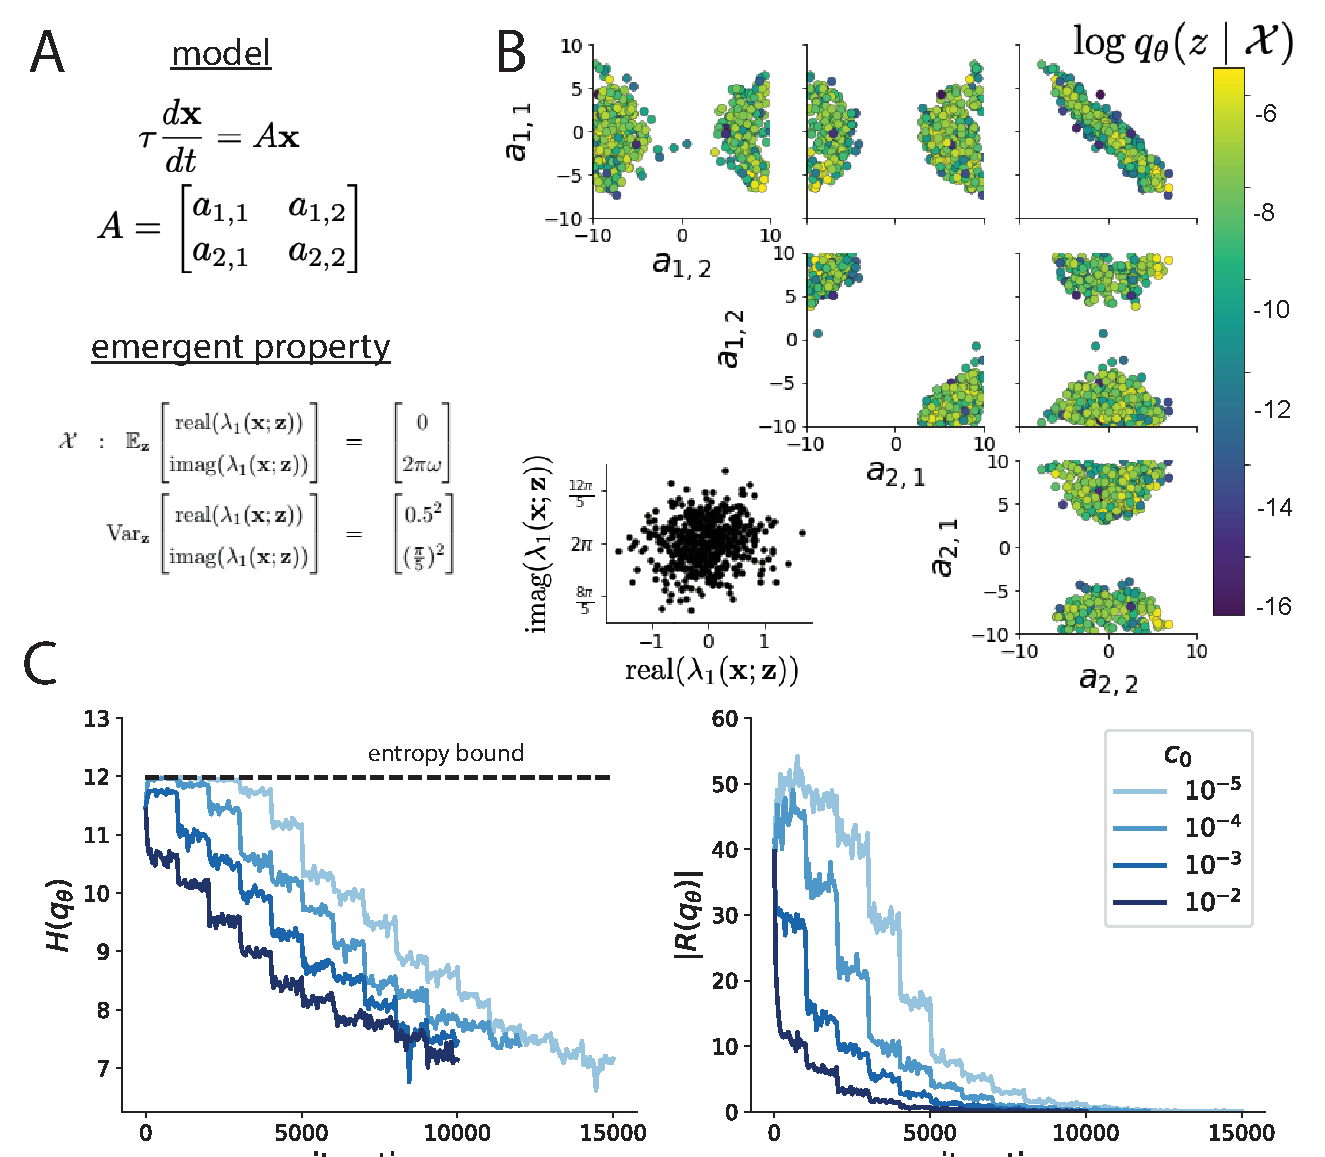
\includegraphics[scale=0.8]{figures/figLDS1/figLDS1.pdf}
\end{center}
\begin{flushleft}
\caption{\small (LDS1): \textbf{A}. Two-dimensional linear dynamical system model, where real entries of the dynamics matrix $A$ are the parameters.  
\textbf{B}. The EPI distribution for a two-dimensional linear dynamical system with $\tau=1$ that produces an average of 1Hz oscillations with some small amount of variance.  Dashed lines indicate the parameter axes. 
\textbf{C}. Entropy throughout the optimization.  
At the beginning of each augmented Lagrangian epoch (2,000 iterations), the entropy dipped due to the shifted optimization manifold where emergent property constraint satisfaction is increasingly weighted.  
\textbf{D}. Emergent property moments throughout optimization.  
At the beginning of each augmented Lagrangian epoch, the emergent property moments adjust closer to their constraints.}
\end{flushleft}
\label{fig:LDS1}
\end{figure}

Unlike the models we presented in the main text, this model admits an analytical form for the mean emergent property statistics given parameter $\mathbf{z}$, since the eigenvalues can be calculated using the quadratic formula: 
\begin{equation}
\lambda = \frac{(\frac{a_1 + a_4}{\tau}) \pm \sqrt{(\frac{a_1+a_4}{\tau})^2 + 4(\frac{a_2 a_3 - a_1 a_4}{\tau})}}{2}.
\end{equation}

Importantly, even though $\mathbb{E}_{\mathbf{x}\sim p(\mathbf{x} \mid \mathbf{z})}\left[T(\mathbf{x})\right]$ is calculable directly via a closed form function and does not require simulation, we cannot derive the distribution $q^*_{\bm{\theta}}$ directly.  
This fact is due to the formally hard problem of the backward mapping: finding the natural parameters $\eta$ from the mean parameters $\bm{\mu}$ of an exponential family distribution \cite{wainwright2008graphical}.  
Instead, we used EPI to approximate this distribution (Fig. S1B). We used a real-NVP normalizing flow architecture with four masks, two neural network layers of 15 units per mask, with batch normalization momentum 0.99, mapped onto a support of $z_i \in \left[-10, 10 \right]$. (see Section \ref{methods_NF}).

Even this relatively simple system has nontrivial (though intuitively sensible) structure in the parameter distribution.  
To validate our method, we analytically derived the contours of the probability density from the emergent property statistics and values.
In the $a_1$-$a_4$ plane, the black line at $\text{real}(\lambda_1) = \frac{a_1 + a_4}{2} = 0$, dotted black line at
the standard deviation $\text{real}(\lambda_1) = \frac{a_1 + a_4}{2} \pm 0.25$, and the dotted gray line at twice the standard deviation
$\text{real}(\lambda_1) = \frac{a_1 + a_4}{2} \pm 0.5$ follow the contour of probability density of the samples (Fig. S2A). 
The distribution precisely reflects the desired statistical constraints and model degeneracy in the sum of $a_1$ and $a_4$.
Intuitively, the parameters equivalent with respect to emergent property statistic $\text{real}(\lambda_1)$ have similar log densities.

\begin{figure}
\begin{center}
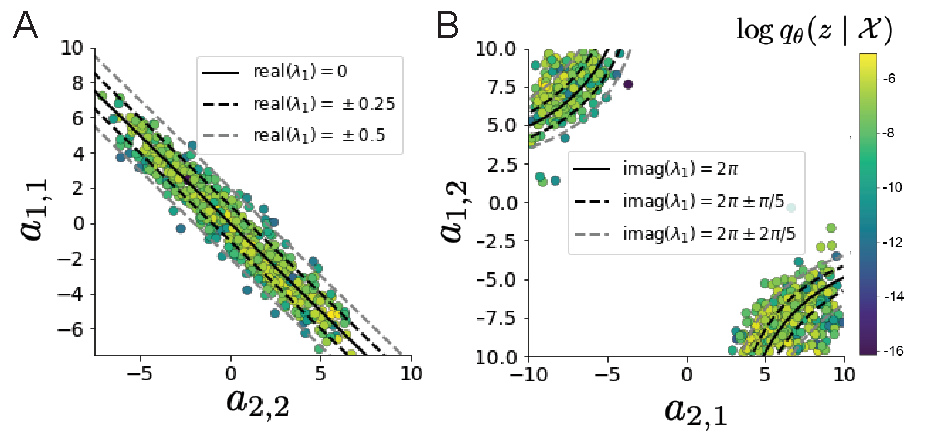
\includegraphics[scale=0.8]{figures/figLDS2/figLDS2.pdf}
\end{center}
\begin{flushleft}
\caption{\small (LDS2): \textbf{A}. Probability contours in the $a_1$-$a_4$ plane were derived from the relationship to emergent property statistic of growth/decay factor $\text{real}(\lambda_1)$. 
\textbf{B}. Probability contours in the $a_2$-$a_3$ plane were derived from the emergent property statistic of oscillation frequency $2\pi \text{imag}(\lambda_1)$.}
\end{flushleft}
\label{fig:LDS2}
\end{figure}

To explain the bimodality of the EPI distribution, we examined the imaginary component of $\lambda_1$.  When $\text{real}(\lambda_1) = \frac{a_1 + a_4}{2} = 0$, we have
\begin{equation}
\text{imag}(\lambda_1) = \begin{cases}
                             \sqrt{\frac{a_1 a_4 - a_2 a_3}{\tau}},  & \text{if } a_1 a_4 < a_2 a_3 \\
                             0 & \text{otherwise } \\
                         \end{cases}.
\end{equation}

When $\tau=1$ and $a_1 a_4 > a_2 a_3$ (center of distribution above), we have the following equation for the other two dimensions:
\begin{equation}
\text{imag}(\lambda_1)^2 = a_1 a_4 - a_2 a_3
\end{equation}
Since we constrained $\mathbb{E}_{\mathbf{z} \sim q_{\bm{\theta}}}\left[\text{imag}(\lambda)\right] = 2 \pi$ (with $\omega=1$), we can plot contours of the equation $\text{imag}(\lambda_1)^2 = a_1 a_4 - a_2 a_3 = (2 \pi)^2$ for various $a_1 a_4$ (Fig. S2B). 
With $\sigma_{1,4} = \mathbb{E}_{\mathbf{z} \sim q_{\bm{\theta}}}(|a_1 a_4 - E_{q_{\bm{\theta}}}[a_1 a_4]|)$, we show the contours as $a_1 a_4 = 0$ (black), $a_1 a_4 = -\sigma_{1,4}$ (black dotted), and $a_1 a_4 = -2\sigma_{1,4}$ (grey dotted). 
This validates the curved structure of the inferred distribution learned through EPI.  
We took steps in negative standard deviation of $a_1 a_4$ (dotted and gray lines), since there are few positive values $a_1 a_4$ in the learned distribution.  
Subtler combinations of model and emergent property will have more complexity, further motivating the use of EPI for understanding these systems.  
As we expect, the distribution results in samples of two-dimensional linear systems oscillating near 1Hz (Fig. S3).

\begin{figure}
\begin{center}
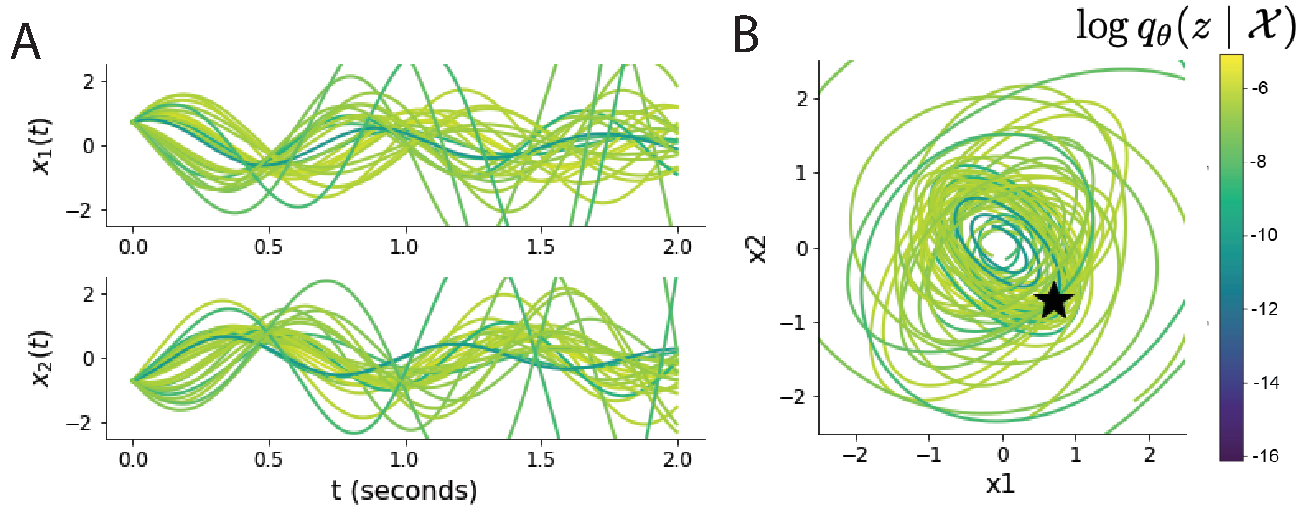
\includegraphics[scale=0.8]{figures/figLDS3/figLDS3.pdf}
\end{center}
\begin{flushleft}
\caption{\small (LDS3): Sampled dynamical systems $\mathbf{z} \sim q_{\bm{\theta}}(\mathbf{z})$ and their simulated activity from $\mathbf{x}(0) = [\frac{\sqrt{2}}{2}, -\frac{\sqrt{2}}{2}]$ colored by log probability. 
\textbf{A}. Each dimension of the simulated trajectories throughout time.  
\textbf{B}.  The simulated trajectories in phase space.}
\end{flushleft}
\label{fig:LDS3}
\end{figure}


\subsubsection{Maximum entropy distributions and exponential families}\label{methods_ME_EF}
%As we compare EPI to variational inference, it is important to consider that EPI is a maximum entropy method, and that maximum entropy methods have a fundamental relationship with exponential family distributions. 
%A maximum entropy distribution of form:
%\begin{equation} \label{eq:max_ent}
%\begin{split}
%p^*(\mathbf{z}) &= \argmax_{p \in \mathcal{P}} H(p(\mathbf{z})) \\
% &  \text{s.t.  } \mathbb{E}_{\mathbf{z} \sim p}\left[T(\mathbf{z})\right] = \bm{\mu}. \\
% \end{split}
%\end{equation} 
%will have probability density in the exponential family:
%\begin{equation}
%p^*(\mathbf{z}) \propto \exp(\bm{\eta}^\top T(\textbf{z})).
%\end{equation}
%The mappings between the mean parameterization $\bm{\mu}$ and the natural parameterization $\bm{\eta}$ are formally hard to identify \cite{wainwright2008graphical}.
EPI is a maximum entropy distribution, which have fundamental links to exponential family distributions. 
A maximum entropy distribution of form:
\begin{equation} \label{eq:max_ent}
\begin{split}
p^*(\mathbf{z}) &= \argmax_{p \in \mathcal{P}} H(p(\mathbf{z})) \\
 &  \text{s.t.  } \mathbb{E}_{\mathbf{z} \sim p}\left[T(\mathbf{z})\right] = \bm{\mu}_{\text{opt}}. \\
 \end{split}
\end{equation} 
will have probability density in the exponential family:
\begin{equation}
p^*(\mathbf{z}) \propto \exp(\bm{\eta}^\top T(\textbf{z})).
\end{equation}
The mappings between the mean parameterization $\bm{\mu}_{\text{opt}}$ and the natural parameterization $\bm{\eta}$ are formally hard to identify except in special cases \cite{wainwright2008graphical}.

In EPI, emergent properties are defined as statistics having a fixed mean and variance as in Equation \ref{eq:EP_STG}.
The variance constraint is a second moment constraint on $f(\mathbf{x}; \mathbf{z})$
 \begin{equation}
\text{Var}_{\mathbf{z},\mathbf{x}}\left[f(\mathbf{x}; \mathbf{z})\right] = \mathbb{E}_{\mathbf{z},\mathbf{x}}\left[\left( f(\mathbf{x}; \mathbf{z}) - \bm{\mu}\right) ^2\right]
\end{equation}
As a general maximum entropy distribution (Equation \ref{eq:max_ent}), the sufficient statistics vector contains both first and second order moments of $f(\mathbf{x}; \mathbf{z})$
\begin{equation} \label{eq:moments}
T(\mathbf{x}; \mathbf{z}) = \begin{bmatrix} f(\mathbf{x}; \mathbf{z}) \\ \left( f(\mathbf{x}; \mathbf{z}) - \bm{\mu} \right)^2 \end{bmatrix},
\end{equation}
which are constrained to the chosen means and variances
\begin{equation} \label{eq:mu_opt}
\bm{\mu}_{\text{opt}} = \begin{bmatrix} \bm{\mu} \\ \bm{\sigma}^2 \end{bmatrix}.
\end{equation}


\subsubsection{EPI as variational inference}\label{methods_VI}
%Now that we have fully described the EPI method, we  consider its broader contextualization as a statistical method and its relation to Bayesian inference. 
In Bayesian inference a prior belief about model parameters $\mathbf{z}$ is stated in a prior distribution $p(\mathbf{z})$, and the statistical model capturing the effect of $\mathbf{z}$ on observed data points $\mathbf{x}$ is formalized in the likelihood distribution $p(\mathbf{x} \mid \mathbf{z})$.
In Bayesian inference, we obtain a posterior distribution $p(\mathbf{z} \mid \mathbf{x})$, which captures how the data inform our knowledge of model parameters using Bayes' rule:
\begin{equation}
p(\mathbf{z} \mid \mathbf{x}) = \frac{p(\mathbf{x} \mid \mathbf{z}) p(\mathbf{z})}{p(\mathbf{x})}.
\end{equation}
The posterior distribution is analytically available when the prior is conjugate with the likelihood.
However, conjugacy is rare in practice, and alternative methods, such as variational inference \cite{saul1998mean}, are utilized.

%Now, consider the goal of doing variational inference with an exponential family posterior distribution $p(z \mid \mathbf{x})$.  
%We use the following abbreviated notation to collect the base measure $b(z)$ and sufficient statistics $T(z)$ into $\tilde{T}(z)$ and likewise concatenate a 1 onto the end of the natural parameter $\tilde{\eta}(\mathbf{x})$.  
%The log normalizing constant $A(\eta(\mathbf{x}))$ remains unchanged:
%\begin{equation}
%\begin{split}
%p(z \mid \mathbf{x}) = b(z) \exp{\left( \eta(\mathbf{x})^\top T(z) - A(\eta(\mathbf{x})) \right)} = \exp{\left( \begin{bmatrix} \eta(\mathbf{x}) \\ 1 \end{bmatrix}^\top \begin{bmatrix} T(z) \\ b(z) \end{bmatrix} - A(\eta(\mathbf{x})) \right)} \\= \exp{\left(\tilde{\eta(\mathbf{x})}^\top \tilde{T}(z) - A(\eta(\mathbf{x})) \right)} 
%\end{split}.
%\end{equation}
%Variational inference with an exponential family posterior distribution uses optimization to minimize the following divergence \cite{blei2017variational}:
%\begin{equation}
%q_{\bm{\theta}}^* = \argmin_{q_{\bm{\theta}} \in Q} KL(q_{\bm{\theta}} \mid \mid p(z \mid \mathbf{x})).
%\end{equation}
%$q_{\bm{\theta}}(z)$ is the variational approximation to the posterior with variational parameters $\bm{\theta}$.  
%We can write this KL divergence in terms of entropy of the variational approximation:
%\begin{equation}
%KL(q_{\bm{\theta}} \mid \mid p(z \mid \mathbf{x})) = \mathbb{E}_{z \sim q_{\bm{\theta}}} \left[ \log (q_{\bm{\theta}}(z)) \right] - \mathbb{E}_{z \sim q_{\bm{\theta}}} \left[ \log (p(z \mid \mathbf{x})) \right]
%\end{equation}
%\begin{equation}
% = -H(q_{\bm{\theta}}) - \mathbb{E}_{z \sim q_{\bm{\theta}}} \left[ \tilde{\eta}(\mathbf{x})^\top  \tilde{T}(z) - A(\eta(\mathbf{x})) \right].
%\end{equation}
%As far as the variational optimization is concerned, the log normalizing constant is independent of $q_{\bm{\theta}}(z)$, so it can be dropped
%\begin{equation}
%\argmin_{q_{\bm{\theta}} \in Q} KL(q_{\bm{\theta}} \mid \mid p(z \mid \mathbf{x})) =  \argmin_{q_{\bm{\theta}} \in Q} -H(q_{\bm{\theta}}) - \mathbb{E}_{z \sim q_{\bm{\theta}}} \left[ \tilde{\eta}(\mathbf{x})^\top  \tilde{T}(z) \right].
%\end{equation}
% Further, we can write the objective in terms of the first moment of the sufficient statistics $\bm{\mu} = \mathbb{E}_{z \sim p(z \mid \mathbf{x})}\left[T(z) \right]$:
% \begin{equation}
%=  \argmin_{q_{\bm{\theta}} \in Q} -H(q_{\bm{\theta}}) - \mathbb{E}_{z \sim q_{\bm{\theta}}} \left[ \tilde{\eta}(\mathbf{x})^\top \left(  \tilde{T}(z) -\bm{\mu} \right) \right] + \tilde{\eta}(\mathbf{x})^\top \bm{\mu},
% \end{equation}
%which simplifies to
%  \begin{equation}
%=  \argmin_{q_{\bm{\theta}} \in Q} -H(q_{\bm{\theta}}) - \mathbb{E}_{z \sim q_{\bm{\theta}}} \left[ \tilde{\eta}(\mathbf{x})^\top \left(  \tilde{T}(z) -\bm{\mu} \right) \right].
% \end{equation}.
%
%In comparison, in emergent property inference (EPI), we solve the following problem:
%\begin{equation}
%q_{\bm{\theta}}^*(z) = \argmax_{q_{\bm{\theta}} \in Q} H(q_{\bm{\theta}}(z)),   \text{  s.t.  } \mathbb{E}_{z \sim q_{\bm{\theta}}}\left[ \mathbb{E}_{\mathbf{x}\sim p(\mathbf{x} \mid z)}\left[T(\mathbf{x})\right] \right] = \bm{\mu}.
%\end{equation}
%The Lagrangian objective (without augmentation) is
%\begin{equation}
%q_{\bm{\theta}}^* = \argmin_{q_{\bm{\theta}} \in Q} - H(q_{\bm{\theta}}) + \eta_{\text{opt}}^\top \left(\mathbb{E}_{z \sim q_{\bm{\theta}}} \left[\tilde{T}(z) \right] - \bm{\mu} \right).
%\end{equation}
%Thus, as the optimization proceeds, $\eta_{\text{opt}}^\top$ should converge to the natural parameter $\tilde{\eta}(\mathbf{x})$ through its adaptations in each epoch (see Section \ref{methods_AL_opt}). 
%
%We have shown that there is indeed a clear relationship between Bayesian inference and EPI.
%Specifically, EPI is executing variational inference in an exponential family posterior,  whose sufficient statistics are the emergent property statistics and mean parameterization are the emergent property values.
%However, in EPI we  have not specified a prior distribution, or collected data, which can inform us about model parameters.
%Instead we have a mathematical specification of an emergent property, which the model must produce, and a maximum entropy selection principle.
%Accordingly, we replace the notation of $p(\mathbf{z} \mid \mathbf{x})$ with $p(\mathbf{z} \mid \mathcal{B})$ conceptualizing an inferred distribution that obeys emergent property $\mathcal{B}$ (see Section \ref{methods_EPI}). 

In variational inference, a posterior approximation $q_{\bm{\theta}}^*$ is chosen from within some variational family $\mathcal{Q}$
\begin{equation}
q_{\bm{\theta}}^*(\mathbf{z}) = \argmin_{q_{\bm{\theta}} \in Q} KL(q_{\bm{\theta}}(\mathbf{z}) \mid \mid p(\mathbf{z} \mid \mathbf{x})).
\end{equation}
The KL divergence can be written in terms of entropy of the variational approximation:
\begin{equation}
KL(q_{\bm{\theta}}(\mathbf{z})  \mid \mid p(\mathbf{z} \mid \mathbf{x})) = \mathbb{E}_{\mathbf{z} \sim q_{\bm{\theta}}} \left[ \log (q_{\bm{\theta}}(\mathbf{z})) \right] - \mathbb{E}_{\mathbf{z} \sim q_{\bm{\theta}}} \left[ \log (p(\mathbf{z} \mid \mathbf{x})) \right]
\end{equation}
\begin{equation}
= -H(q_{\bm{\theta}}) - \mathbb{E}_{\mathbf{z} \sim q_{\bm{\theta}}} \left[ \log (p(\mathbf{x} \mid \mathbf{z}))  + \log(p(\mathbf{z})) - \log(p(\mathbf{x}))\right]
\end{equation}
Since the marginal distribution of the data $p(\mathbf{x})$ (or ``evidence") is independent of $\bm{\theta}$, variational inference is executed by optimizing the remaining expression.
This is usually framed as maximizing the evidence lower bound (ELBO)
\begin{equation}
\argmin_{q_{\bm{\theta}} \in Q} KL(q_{\bm{\theta}} \mid \mid p(\mathbf{z} \mid \mathbf{x})) = \argmax_{q_{\bm{\theta}} \in Q} H(q_{\bm{\theta}}) + \mathbb{E}_{\mathbf{z} \sim q_{\bm{\theta}}} \left[ \log (p(\mathbf{x} \mid \mathbf{z}))  + \log(p(\mathbf{z}))\right].
\end{equation}

Now, consider the setting where we have chosen a uniform prior, and stipulate a mean-field gaussian likelihood on a chosen statistic of the data $f(\mathbf{x}; \mathbf{z})$
\begin{equation}
p(\mathbf{x} \mid \mathbf{z}) = \mathcal{N}(f(\mathbf{x}; \mathbf{z}) \mid \bm{\mu}_f, \Sigma_f),
\end{equation}
where $\Sigma_f = \text{diag}(\bm{\sigma}_f^2)$.
The log likelihood is then proportional to a dot product of the natural parameter of this mean-field gaussian distribution and the first and second moment statistics.
\begin{equation}
\log p(\mathbf{x} \mid \mathbf{z}) \propto \bm{\eta}_f^\top T(\mathbf{x}, \mathbf{z}),
\end{equation}
where
\begin{equation} 
\label{eq:eta_f}
\bm{\eta}_{f} = \begin{bmatrix} \frac{\bm{\mu}_f}{\bm{\sigma}_f^2} \\ \frac{-1}{2\bm{\sigma}_f^2} \end{bmatrix}, \text{ and}
\end{equation}
\begin{equation}
T(\mathbf{x}; \mathbf{z}) = \begin{bmatrix} f(\mathbf{x}; \mathbf{z}) \\ \left( f(\mathbf{x}; \mathbf{z}) - \bm{\mu}_f \right)^2 \end{bmatrix}.
\end{equation}
The variational objective is then
\begin{equation}
\label{eq:VI_obj}
\argmax_{q_{\bm{\theta}} \in Q} H(q_{\bm{\theta}}) + \bm{\eta}_f^\top \mathbb{E}_{\mathbf{z} \sim q_{\bm{\theta}}}\left[ T(\mathbf{x}; \mathbf{z}) \right]
\end{equation}

Comparing this to the Lagrangian objective (without augmentation) of EPI, we see they are the same
\begin{equation}
\begin{split}
q_{\bm{\theta}}^*(\mathbf{z}) &= \argmin_{q_{\bm{\theta}} \in Q} - H(q_{\bm{\theta}}) + \bm{\eta}_{\text{opt}}^\top \left(\mathbb{E}_{\mathbf{z}, \mathbf{x}} \left[T(\mathbf{x}; \mathbf{z}) \right] - \bm{\mu}_{\text{opt}} \right) \\
 &= \argmin_{q_{\bm{\theta}} \in Q} - H(q_{\bm{\theta}}) + \bm{\eta}_{\text{opt}}^\top \mathbb{E}_{\mathbf{z}, \mathbf{x}} \left[T(\mathbf{x}; \mathbf{z}) \right].
\end{split}
\end{equation}
where $T(\mathbf{x}; \mathbf{z})$ consists of the first and second moments of the emergent property statistic $f(\mathbf{x}; \mathbf{z})$ (Equation \ref{eq:moments}).
Thus, EPI is implicitly executing variational inference with a uniform prior and a mean-field gaussian likelihood on the emergent property statistics.
The mean and variances of the mean-field gaussian likelihood are predicated by $\bm{\eta}_{\text{opt}}$ (Equations \ref{eq:eta_f} and \ref{eq:VI_obj}), which is adapted after each EPI optimization epoch based on $\mathcal{X}$ (see Section \ref{methods_AL_opt}).
In EPI, the inferred distribution is not conditioned on a finite dataset as in variational inference, but rather the emergent property $\mathcal{X}$ dictates the likelihood parameterization such that the inferred distribution will produce the emergent property.
As a note, we could not simply choose $\bm{\mu}_f$ and $\bm{\sigma}_f$ directly from the outset, since we do not know which of these choices will produce the emergent property $\mathcal{X}$, which necessitates the EPI optimization routine that adapts $\bm{\eta}_{\text{opt}}$.
Accordingly, we replace the notation of $p(\mathbf{z} \mid \mathbf{x})$ with $p(\mathbf{z} \mid \mathcal{X})$ conceptualizing an inferred distribution that obeys emergent property $\mathcal{X}$ (see Section \ref{methods_EPI}). 

\subsection{Theoretical models}\label{methods_theoretical_models}
In this study, we used emergent property inference to examine several theoretical models of computation.
Here, we provide the details of each model and the related analyses.

\subsubsection{Stomatogastric ganglion}\label{methods_STG}
We analyze how the parameters $\mathbf{z} = [ g_{\text{el}}, g_{\text{synA}}]$ govern the emergent phenomena of intermediate hub frequency in a model of the stomatogastric ganglion (STG) \cite{gutierrez2013multiple} shown in Figure \ref{fig:STG}A with activity $\mathbf{x} = \left[ x_{\text{f1}}, x_{\text{f2}}, x_{\text{hub}}, x_{\text{s1}}, x_{\text{s2}} \right]$, using the same hyperparameter choices as Gutierrez et al.
Each neuron's membrane potential $x_\alpha(t)$ for $\alpha \in \{ \text{f1}, \text{f2}, \text{hub}, \text{s1}, \text{s2} \}$ is the solution of the following stochastic differential equation:
\begin{equation} C_m \frac{dx_\alpha}{dt} = - \left[ h_{leak}(\mathbf{x}; \mathbf{z}) + h_{Ca}(\mathbf{x}; \mathbf{z}) + h_K(\mathbf{x}; \mathbf{z}) + h_{hyp}(\mathbf{x}; \mathbf{z}) + h_{elec}(\mathbf{x}; \mathbf{z}) + h_{syn}(\mathbf{x}; \mathbf{z})\right] + dB.
\end{equation} 
The input current of each neuron is the sum of the leak, calcium, potassium, hyperpolarization, electrical and synaptic currents as well as gaussian noise $dB$.
Each current component is a function of all membrane potentials and the conductance parameters $\mathbf{z}$.

The capacitance of the cell membrane was set to $C_m = 1nF$. Specifically, the currents are the difference in the neuron's membrane potential and that current type's reversal potential multiplied by a conductance:
\begin{equation}  h_{leak}(\mathbf{x}; \mathbf{z}) = g_{leak} (x_\alpha - V_{leak}) 
\end{equation} 
\begin{equation}  h_{elec}(\mathbf{x}; \mathbf{z}) = g_{\text{el}} (x_\alpha^{post} - x_\alpha^{pre})
\end{equation} 
\begin{equation}  h_{syn}(\mathbf{x}; \mathbf{z}) = g_{syn} S_\infty^{pre} (x_\alpha^{post} - V_{syn}) \end{equation} 
\begin{equation}  h_{Ca}(\mathbf{x}; \mathbf{z}) = g_{Ca} M_\infty (x_\alpha - V_{Ca}) 
\end{equation} 
\begin{equation}  h_K(\mathbf{x}; \mathbf{z}) = g_K N (x_\alpha - V_K) 
\end{equation} 
\begin{equation}  h_{hyp}(\mathbf{x}; \mathbf{z}) = g_h H(x_\alpha - V_{hyp}).
\end{equation} 
The reversal potentials were set to $V_{leak} = -40mV$, $V_{Ca} = 100mV$, $V_K = -80mV$, $V_{hyp} = -20mV$, and $V_{syn} = -75mV$.  
The other conductance parameters were fixed to $g_{leak} = 1 \times 10^{-4} \mu S$. $g_{Ca}$, $g_{K}$, and $g_{hyp}$ had different values based on fast, intermediate (hub) or slow neuron.  
The fast conductances had values $g_{Ca} = 1.9 \times 10^{-2}$, $ g_K = 3.9 \times 10^{-2} $, and $ g_{hyp} = 2.5 \times 10^{-2} $.  
The intermediate conductances had values $g_{Ca} = 1.7 \times 10^{-2}$, $ g_K = 1.9 \times 10^{-2} $, and $ g_{hyp} = 8.0 \times 10^{-3} $.  
Finally, the slow conductances had values $g_{Ca} = 8.5 \times 10^{-3}$, $ g_K = 1.5 \times 10^{-2} $, and $ g_{hyp} = 1.0 \times 10^{-2} $.

Furthermore, the Calcium, Potassium, and hyperpolarization channels have time-dependent gating dynamics dependent on steady-state gating variables $M_\infty$, $N_\infty$ and $H_\infty$, respectively:
\begin{equation}  M_{\infty} = 0.5 \left( 1 + \tanh \left( \frac{x_\alpha - v_1}{v_2} \right) \right) \end{equation}
\begin{equation}  \frac{dN}{dt} = \lambda_N (N_\infty - N)  \end{equation}
\begin{equation}  N_\infty = 0.5 \left( 1 + \tanh \left( \frac{x_\alpha - v_3}{v_4} \right) \right) \end{equation}
\begin{equation}  \lambda_N = \phi_N \cosh \left( \frac{x_\alpha - v_3}{2 v_4} \right) \end{equation}
\begin{equation}  \frac{dH}{dt} = \frac{\left( H_\infty - H \right)}{\tau_h} \end{equation}
\begin{equation}  H_\infty = \frac{1}{1 + \exp \left( \frac{x_\alpha + v_5}{v_6} \right)} \end{equation}
\begin{equation}  \tau_h = 272 - \left( \frac{-1499}{1 + \exp \left( \frac{-x_\alpha + v_7}{v_8} \right)} \right).
 \end{equation}
where we set $v_1 = 0mV$, $v_2  = 20mV$, $v_3 = 0mV$, $v_4 = 15mV$, $v_5 = 78.3mV$,
$v_6 = 10.5mV$, $v_7 = -42.2mV$, $v_8 = 87.3mV$, $v_9 = 5mV$, and $v_{th} = -25mV$.  

Finally, there is a synaptic gating variable as well:
\begin{equation} S_\infty = \frac{1}{1 + \exp \left( \frac{v_{th} - x_\alpha}{v_9} \right)} .
\end{equation}
When the dynamic gating variables are considered, this is actually a 15-dimensional nonlinear dynamical system.  Gaussian noise $d\mathbf{B}$ of variance $(1 \times 10^{-12})^2$ A$^2$ makes the model stochastic, and introduces variability in frequency at each parameterization $\mathbf{z}$.

In order to measure the frequency of the hub neuron during EPI, the STG model was simulated for $T = 300$ time steps of $dt = 25\text{ms}$.  
The chosen $dt$ and $T$ were the most computationally convenient choices yielding accurate frequency measurement.  
We used a basis of complex exponentials with frequencies from 0.0-1.0 Hz at 0.01Hz resolution to measure frequency from simulated time series
\begin{equation}
\Phi = \left[ 0.0, 0.01, ..., 1.0 \right]^\top..
\end{equation}

To measure spiking frequency, we processed simulated membrane potentials with a relu (spike extraction) and low-pass filter with averaging window of size 20, then took the frequency with the maximum absolute value of the complex exponential basis coefficients of the processed time-series.  The first 20 temporal samples of the simulation are ignored to account for initial transients.

To differentiate through the maximum frequency identification, we used a soft-argmax
Let $X_\alpha \in \mathcal{C}^{|\Phi|}$ be the complex exponential filter bank dot products with the signal $x_\alpha \in \mathbb{R}^{N}$, where $\alpha \in \{ \text{f1}, \text{f2}, \text{hub}, \text{s1}, \text{s2} \}$.  
The soft-argmax is then calculated using temperature parameter $\beta=100$
\begin{equation}
\psi_\alpha = \text{softmax}(\beta|X_\alpha|\odot i),
\end{equation}
where $i = [0, 1, ..., 100]$.
The frequency is then calculated as 
\begin{equation}
\omega_\alpha = 0.01\psi_\alpha \text{Hz}.
\end{equation}

Intermediate hub frequency, like all other emergent properties in this work, is defined by the mean and variance of the emergent property statistics.
In this case, we have one statistic, hub neuron frequency, where the mean was chosen to be 0.55Hz, and variance was chosen to be (0.025Hz)$^2$ (Equation \ref{eq:EP_STG}).
As a maximum entropy distribution, $T(\mathbf{x}, \mathbf{z})$ is comprised of both these first and second moments of the hub neuron frequency (as in Equations \ref{eq:moments} and \ref{eq:mu_opt})
\begin{equation} 
T(\mathbf{x}; \mathbf{z}) = \begin{bmatrix} \omega_{\text{hub}}(\mathbf{x}; \mathbf{z}) \\ \left( \omega_{\text{hub}}(\mathbf{x}; \mathbf{z}) - 0.55 \right)^2 \end{bmatrix},
\end{equation}
\begin{equation} 
\bm{\mu}_{\text{opt}} = \begin{bmatrix} 0.55 \\ 0.025^2 \end{bmatrix}.
\end{equation}
Throughout optimization, the augmented Lagrangian parameters $\eta$ and $c$, were updated after each epoch of 5,000 iterations(see Section \ref{methods_AL_opt}).  
The optimization converged after five epochs (Fig. S4).

\begin{figure}
\begin{center}
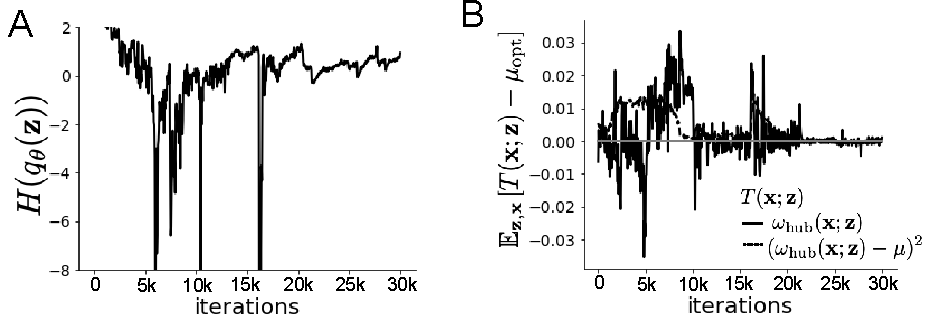
\includegraphics[scale=0.8]{figures/figSTG1/figSTG1.pdf}
\end{center}
\begin{flushleft}
\caption{\small (STG1): EPI optimization of the STG model producing network syncing. 
\textbf{A}. Entropy throughout optimization. 
\textbf{B}. The emergent property statistic means and variances converge to their constraints at 25,000 iterations following the fifth augmented Lagrangian epoch.}
\end{flushleft}
\label{fig:STG1}
\end{figure}

For EPI in Fig \ref{fig:STG}E, we used a real NVP architecture with three Real NVP coupling layers and two-layer neural networks of 25 units per layer.
The normalizing flow architecture mapped $z_0 \sim \mathcal{N}(\mathbf{0}, I)$ to a support of $\mathbf{z} = [g_{\text{el}}, g_{\text{synA}}] \in [4,8] \times [0.01,4]$, initialized to a gaussian approximation of samples returned by a preliminary ABC search.
We did not include $g_{\text{synA}} < 0.01$, for numerical stability.
EPI optimization was run using 5 different random seeds for architecture initialization $\bm{\theta}$ with an augmented Lagrangian coefficient of $c_0 = 10^{5}$, a batch size $n=400$, and $\beta = 2$.
The architecture converged with criteria $N_{\text{test}} = 100$.

In Figure \ref{fig:STG}D, the sensitivity dimension $v_1$ (solid) and the second eigenvector of the Hessian $v_2$ (dashed) are shown evaluated at the mode of the distribution.  
The length of the arrows is inversely proportional to the square root of the absolute value of their eigenvalues $\lambda_1 = -10.7$ and $\lambda_2 = -3.22$.
Since the Hessian eigenvectors have sign degeneracy, the visualized directions in 2-D parameter space were chosen to have positive $g_{\text{synA}}$.$  $
%We quantitatively measured the sensitivity of the model with respect to network syncing along the eigenvectors of the Hessian (Fig. \ref{fig:STG}B, inset).
%Sensitivity was measured as the slope coefficient of linear regression fit to network syncing error (the sum of squared differences of each neuron's frequency from 0.53Hz) as a function of parametric perturbation magnitude (maximum 0.25) away from the mode along both orientations indicated by the eigenvector with 100 equally spaced samples.
%The sensitivity slope coefficient of eigenvector $v_1$ with respect to network syncing was significant ($\beta = 4.82 \times 10^{-2}$, $p<10^{-4}$).
%In contrast, eigenvector $v_2$ did not identify a dimension of parameter space significantly sensitive to network syncing ($\beta = 8.65 \times 10^{-4}$ with $p=.67$).
%These sensitivities were compared to all other dimensions of parameter space (100 equally spaced angles from 0 to $\pi$), revealing that the Hessian eigenvectors indeed identified the directions of greatest sensitivity and degeneracy (Fig. \ref{fig:STG}B, inset).
%The contours of Figure \ref{fig:STG} were calculated as error in $T(\mathbf{x})$ from $\mu$ in both the first and second moment emergent property statistics.

\subsubsection{Scaling EPI for stable amplification in RNNs}\label{methods_RNN}
We examined the scaling properties of EPI by learning connectivities of RNNs of increasing size that exhibit stable amplification.
Rank-2 RNN connectivity was modeled as $W = UV^\top$, where $U = \begin{bmatrix} \mathbf{u}_1 & \mathbf{u}_2 \end{bmatrix} + g \chi^{(W)}$, $V = \begin{bmatrix} \mathbf{v}_1 & \mathbf{v}_2 \end{bmatrix} + g\chi^{(V)}$, and $\chi^{(W)}_{i,j}, \chi^{(V)}_{i,j} \sim \mathcal{N}(0, 1)$.
This RNN model has dynamics
\begin{equation}
\tau \dot{\mathbf{x}} = -\mathbf{x} + W\mathbf{x}.
\end{equation}
In this analysis, we inferred connectivity parameterizations $\mathbf{z} = \left[\mathbf{u}_1^\top, \mathbf{u}_2^\top, \mathbf{v}_1^\top, \mathbf{v}_2^\top \right]^\top \in \left[-1, 1 \right]^{(4N)}$   that produced stable amplification using EPI, SMC-ABC \cite{sisson2007sequential}, and SNPE \cite{gonccalves2019training} (see Section Related Methods).

For this RNN model to be stable, all real eigenvalues of $W$ must be less than 1:  $\text{real}(\lambda_1) < 1$, where $\lambda_1$ denotes the greatest real eigenvalue of $W$.
For a stable RNN to amplify at least one input pattern, the symmetric connectivity $W^s = \frac{W + W\top}{2}$ must have an eigenvalue greater than 1:
$\lambda^s_1 > 1$, where  $\lambda^s$ is the maximum eigenvalue of $W^s$.
These two conditions are necessary and sufficient for stable amplification in RNNs \cite{bondanelli2020coding}.
We defined the emergent property of stable amplification with means of these eigenvalues (0.5 and 1.5, respectively) that satisfy these conditions.
To complete the emergent property definition, we chose variances ($0.25^2$) about those means such that samples rarely violate the eigenvalue constraints.
In terms of the EPI optimization variables, this is written as
\begin{equation} 
T(\mathbf{x}; \mathbf{z}) = \begin{bmatrix} \text{real}(\lambda_1)(\mathbf{x}; \mathbf{z}) \\ \lambda_1^s(\mathbf{x}; \mathbf{z}) \\ \left(\text{real}(\lambda_1)(\mathbf{x}; \mathbf{z}) - 0.5 \right)^2 \\ \left( \lambda_1^s(\mathbf{x}; \mathbf{z})  - 1.5 \right)^2 \end{bmatrix},
\end{equation}
\begin{equation} 
\bm{\mu}_{\text{opt}} = \begin{bmatrix} 0.5 \\ 1.5 \\ 0.25^2 \\ 0.25^2 \end{bmatrix}.
\end{equation}
Gradients of maximum eigenvalues of Hermitian matrices like $W^s$ are available with modern automatic differentiation tools.
To differentiate through the $\text{real}(\lambda_1)$, we solved the following equation for eigenvalues of rank-2 matrices using the rank reduced matrix $W^r = V^{\top} U$
\begin{equation}
\lambda_{\pm} = \frac{\text{Tr}(W^r) \pm \sqrt{\text{Tr}(W^r)^2 - 4\text{Det}(W^r)}}{2}.
\end{equation}

For EPI in Fig. \ref{fig:LRRNN}, we used a real NVP architecture with three coupling layers of affine transformations parameterized by two-layer neural networks of 100 units per layer.
The initial distribution was a standard isotropic gaussian $z_0 \sim \mathcal{N}(\mathbf{0}, I)$ mapped to the support of $\mathbf{z}_i \in [-1, 1]$. 
We used an augmented Lagrangian coefficient of $c_0 = 10^{3}$, a batch size $n=200$, $\beta=4$, and chose to use $500$ iterations per augmented Lagrangian epoch and emergent property constraint convergence was evaluated at $N_{\text{test}} = 200$ (Fig. \ref{fig:LRRNN}B blue line, and Fig. \ref{fig:LRRNN}C-D blue).

We compared EPI to two alternative simulation-based inference techniques, since the likelihood of these eigenvalues given $\mathbf{z}$ is not available.
Approximate Bayesian computation (ABC) \cite{beaumont2002approximate} is a rejection sampling technique for obtaining sets of parameters $\mathbf{z}$ that produce activity $\mathbf{x}$ close to some observed data $\mathbf{x}_0$.
Sequential Monte Carlo approximate Bayesian computation (SMC-ABC) is the state-of-the-art ABC method, which leverages SMC techniques to improve sampling speed.
We ran SMC-ABC with the pyABC package \cite{klinger2018pyabc} to infer RNNs with stable amplification: connectivities having eigenvalues within an $\epsilon$-defined $l$-$2$ distance of
\begin{equation}\label{eq:stab_amp_x0}
x_0 = \begin{bmatrix} \text{real}(\lambda_1) \\ \lambda^s_1 \end{bmatrix} = \begin{bmatrix} 0.5 \\ 1.5 \end{bmatrix}.
\end{equation}
SMC-ABC was run with a uniform prior over $\mathbf{z} \in \left[-1, 1 \right]^{(4N)}$, a population size of 1,000 particles with simulations parallelized over 32 cores, and a multivariate normal transition model.

\begin{figure}
\begin{center}
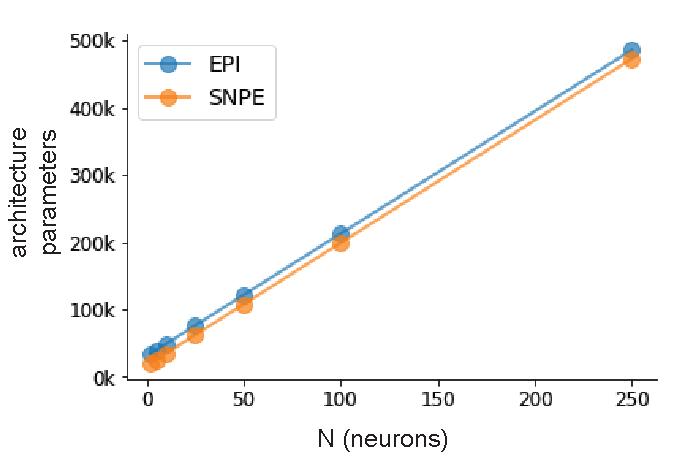
\includegraphics[scale=0.7]{figures/figRNN1/figRNN1.pdf}
\end{center}
\caption{\small (RNN1): 
Number of parameters in deep probability distribution architectures of EPI (blue) and SNPE (orange) by RNN size ($N$).
}
\label{fig:RNN1}
\end{figure}

SNPE, the next approach in our comparison, is far more similar to EPI.
Like EPI, SNPE treats parameters in mechanistic models with deep probability distributions, yet the two learning algorithms are categorically different.
SNPE uses a two-network architecture to approximate the posterior distribution of the model conditioned on observed data $\mathbf{x}_0$.
The amortizing network maps observations $\mathbf{x}_i$ to the parameters of the deep probability distribution. 
The weights and biases of the parameter network are optimized by sequentially augmenting the training data with additional pairs ($\mathbf{z}_i$, $\mathbf{x}_i$) based on the most recent posterior approximation.
This sequential procedure is important to get training data $\mathbf{z}_i$ to be closer to the true posterior, and $\mathbf{x}_i$ to be closer to the observed data.
For the deep probability distribution architecture, we chose a masked autoregressive flow with affine couplings (the default choice), three transforms, 50 hidden units, and a normalizing flow mapping to the support as in EPI.
This architectural choice closely tracked the size of the architecture used by EPI (Fig. \ref{fig:RNN1}).
As in SMC-ABC, we ran SNPE with $\mathbf{x}_0 = \mu$.
All SNPE optimizations were run for a limit of 1.5 days on a Tesla V100 GPU, or until two consecutive rounds resulted in a validation log probability lower than the maximum observed for that random seed.

\begin{figure}
\begin{center}
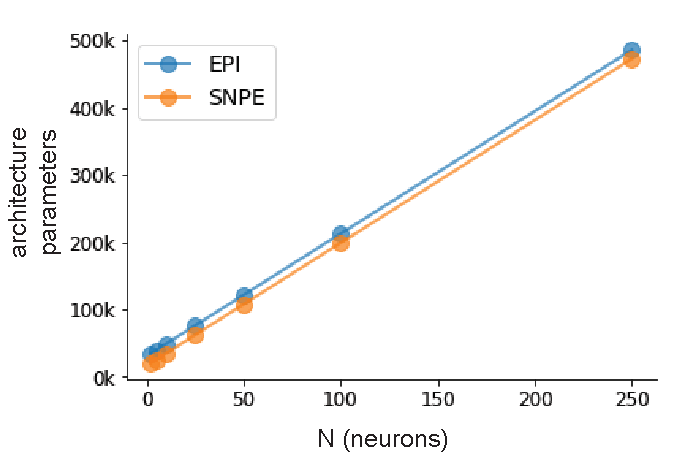
\includegraphics[scale=0.8]{figures/figRNN2/figRNN2.pdf}
\end{center}
\caption{\small (RNN2): Model characteristics affect predictions of posteriors inferred by SNPE, while predictions of parameters inferred by EPI remain fixed.
\textbf{A}. Predictive distribution of EPI (blue) and SNPE (orange) inferred connectivity of RNNs exhibiting stable amplification with $N=2$ (top), $N=10$ (bottom), $g=0.01$ (left), and $g=0.1$ (right).
\textbf{B}. Entropy of parameter distribution approximations throughout optimization with $N=2$ (top), $N=10$ (bottom), $g=0.1$ (dark shade), and $g=0.01$ (light shade).
\textbf{C}. Validation log probabilities throughout SNPE optimization. Same conventions as B.
\textbf{D}. Adherence to EPI constraints. Same conventions as B.
}
\label{fig:RNN2}
\end{figure}

To clarify the difference in objectives of EPI and SNPE, we show their results on RNN models with different numbers of neurons $N$ and random strength $g$.  
The parameters inferred by EPI consistently produces the same mean and variance of $\text{real}(\lambda_1)$ and $\lambda_1^s$, while those inferred by SNPE change according to the model definition (Fig. \ref{fig:RNN2}A).
For $N=2$ and $g=0.01$, the SNPE posterior has greater concentration in eigenvalues around $\mathbf{x}_0$ than at $g=0.1$, where the model has greater randomness (Fig. \ref{fig:RNN2}B top, orange).
At both levels of $g$ when $N=2$, the posterior of SNPE has lower entropy than EPI at convergence (Fig. \ref{fig:RNN2}B top).
However at $N=10$, SNPE results in a predictive distribution of more widely dispersed eigenvalues (Fig. \ref{fig:RNN2}A bottom), and an inferred posterior with greater entropy than EPI (Fig. \ref{fig:RNN2}B bottom).
We highlight these differences not to focus on an insightful trend, but to emphasize that these methods optimize different objectives with different implications.

Note that SNPE converges when it's validation log probability has saturated after several rounds of optimization (Fig. \ref{fig:RNN2}C), and that EPI converges after several epochs of its own optimization to enforce the emergent property constraints (Fig. \ref{fig:RNN2}D blue).
Importantly, as SNPE optimizes its posterior approximation, the predictive means change, and at convergence may be different than $\mathbf{x}_0$ (Fig. \ref{fig:RNN2}D orange, left).
It is sensible to assume that predictions of a well-approximated SNPE posterior should closely reflect the data on average (especially given a uniform prior and a low degree of stochasticity), however this is not a given.
Furthermore, no aspect of the SNPE optimization controls the variance of the predictions (Fig. \ref{fig:RNN2}D orange, right).

To compare the efficiency of these algorithms for inferring RNN connectivity distributions producing stable amplification, we develop a convergence criteria that can be used across methods.
While EPI has its own hypothesis testing convergence criteria for the emergent property, it would not make sense to use this criteria on SNPE and SMC-ABC which do not constrain the means and variances of their predictions.
Instead, we consider EPI and SNPE to have converged after completing its most recent optimization epoch (EPI) or round (SNPE) in which the distance
\begin{equation}
d(q_\theta(z)) = |\mathbb{E}_{\mathbf{z}, \mathbf{x}} \left[f(\mathbf{x}; \mathbf{z}) \right] - \bm{\mu}|_2
\end{equation}
is less than 0.5.
We consider SMC-ABC to have converged once the population produces samples within the $\epsilon = 0.5$ ball ensuring stable amplification.

\begin{figure}
\begin{center}
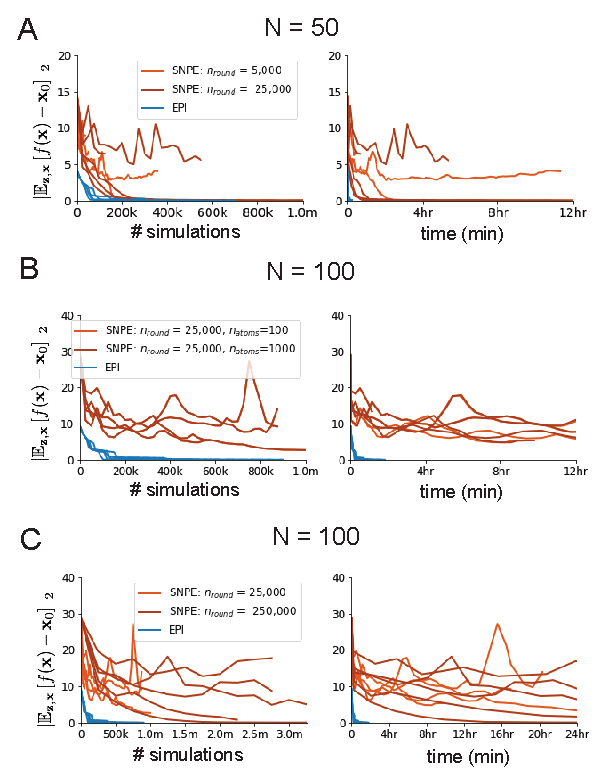
\includegraphics[scale=1.]{figures/figRNN3/figRNN3.pdf}
\end{center}
\caption{\small (RNN3): 
SNPE convergence was enabled by increasing $n_{\text{round}}$, not $n_{\text{atom}}$.
\textbf{A}. Difference of mean predictions $\mathbf{x}_0$ throughout optimization at $N=50$ with by simulation count (left) and wall time (right) of SNPE with $n_{\text{round}} = 5,000$ (light orange), SNPE with $n_{\text{round}} = 25,000$ (dark orange), and EPI (blue).
Each line shows an individual random seed.
\textbf{B}. Same conventions as A at $N=100$ of SNPE with $n_{\text{atom}} = 100$ (light orange) and $n_{\text{atom}} = 1,000$ (dark orange).
\textbf{C}. Same conventions as A at $N=100$ of SNPE with $n_{\text{round}} = 25,000$ (light orange) and $n_{\text{round}} = 250,000$ (dark orange).
}
\label{fig:RNN3}
\end{figure}

When assessing the scalability of SNPE, it is important to check that alternative hyperparamterizations could not yield better performance.
Key hyperparameters of the SNPE optimization are the number of simulations per round $n_{\text{round}}$, the number of atoms used in the atomic proposals of the SNPE-C algorithm \cite{greenberg2019automatic}, and the batch size $n$.
To match EPI, we used a batch size of $n = 200$ for $N <= 25$, however we found $n=1,000$ to be helpful for SNPE in higher dimensions.
While $n_{\text{round}} = 1,000$ yielded SNPE convergence for $N <= 25$, we found that a substantial increase to $n_{\text{round}} = 25,000$ yielded more consistent convergence at $N=50$ (Fig. \ref{fig:RNN3}A).
By increasing $n_{\text{round}}$, we also necessarily increase the duration of each round.
At $N=100$, we tried two hyperparameter modifications.
As suggested in \cite{greenberg2019automatic}, we increased $n_{\text{atom}}$ by an order of magnitude to improve gradient quality, but this had little effect on the optimization (much overlap between same random seeds) (Fig. \ref{fig:RNN3}B).
Finally, we increased $n_{\text{round}}$ by an order of magnitude, which yielded convergence in one case, but no others.
We found no way to improve the convergence rate of SNPE without making more aggressive hyperparameter choices requiring high numbers of simulations.

In Figure \ref{fig:LRRNN}C-D, we show samples form the random seed resulting in emergent property convergence at greatest entropy (EPI), the random seed resulting in greatest validation log probability (SNPE), and the result of all converged random seeds (SMC).


\subsubsection{Primary visual cortex}\label{methods_V1}
In the stochastic stabilized supralinear network \cite{hennequin2018dynamical}, population rate responses $\mathbf{x}$ to input $\mathbf{h}$, recurrent input $W\mathbf{x}$ and slow noise $\bm{\epsilon}$ are governed by
\begin{equation}
    \tau \frac{d\mathbf{x}}{dt} = -\mathbf{x} +\phi(W\mathbf{x} + \mathbf{h} + \bm{\epsilon}),
\end{equation}
where the noise is an Ornstein-Uhlenbeck process $\bm{\epsilon} \sim OU(\tau_{\text{noise}}, \bm{\sigma})$
\begin{equation}
\tau_{\text{noise}} d\epsilon_\alpha = -\epsilon_\alpha dt + \sqrt{2\tau_{\text{noise}}}\tilde{\sigma}_\alpha dB
\end{equation}
with $\tau_{\text{noise}} = 5\text{ms} > \tau = 1\text{ms}$.
The noisy process is parameterized as
\begin{equation}
\tilde{\sigma}_\alpha = \sigma_\alpha \sqrt{1 + \frac{\tau}{\tau_{\text{noise}}}},
\end{equation}
so that $\bm{\sigma}$ parameterizes the variance of the noisy input in the abscence of recurrent connectivity ($W = \bm{0}$).
As contrast $c \in [0, 1]$ increases, input to the E- and P-populations increases  relative to a baseline input $\mathbf{h} = \mathbf{h}_b + c\mathbf{h}_c$.
Connectivity ($W_{\text{fit}}$) and input ($\mathbf{h}_{b,\text{fit}}$ and $\mathbf{h}_{c,\text{fit}}$) parameters were fit using the deterministic V1 circuit model \cite{palmigiano2020structure} 

\begin{figure}
\begin{center}
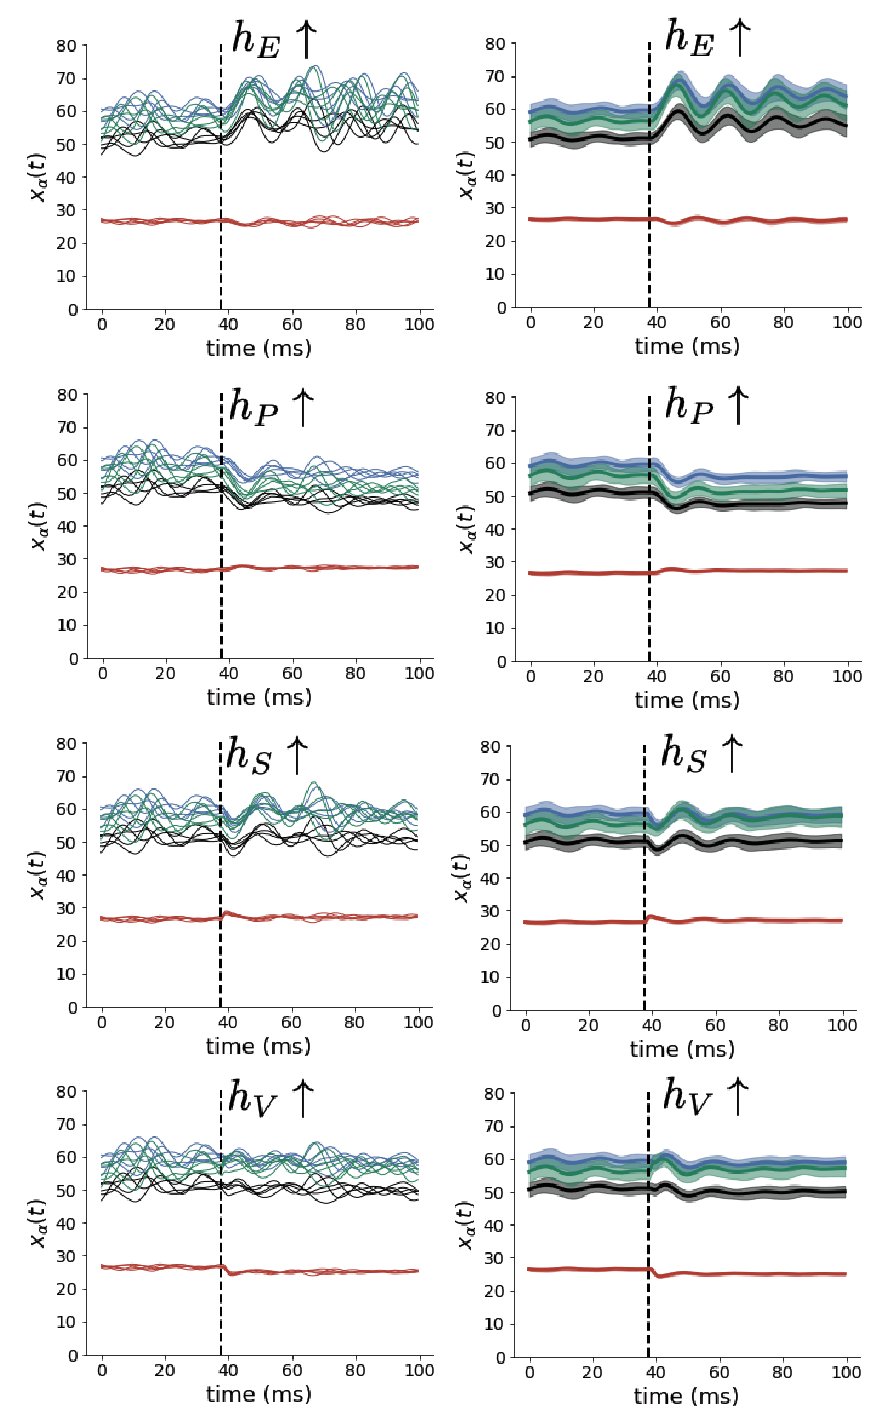
\includegraphics[scale=.8]{figures/figV1_1/figV1_1.pdf}
\end{center}
\caption{\small (V1 1)
(Left) Simulations for small increases in neuron-type population input.
Input magnitudes are chosen so that effect is salient ($0.002$ for E and P, but $0.02$ for S and V).
(Right) Average (solid) and standard deviation (shaded) of stochastic fluctuations of responses.
 }
 \label{fig:V1_1}
\end{figure}

\begin{figure}
\caption{\small (V1 2)
EPI predictive distributions of the sum of squares of each pair of noise parameters.
 }
 \label{fig:V1_2}
\begin{center}
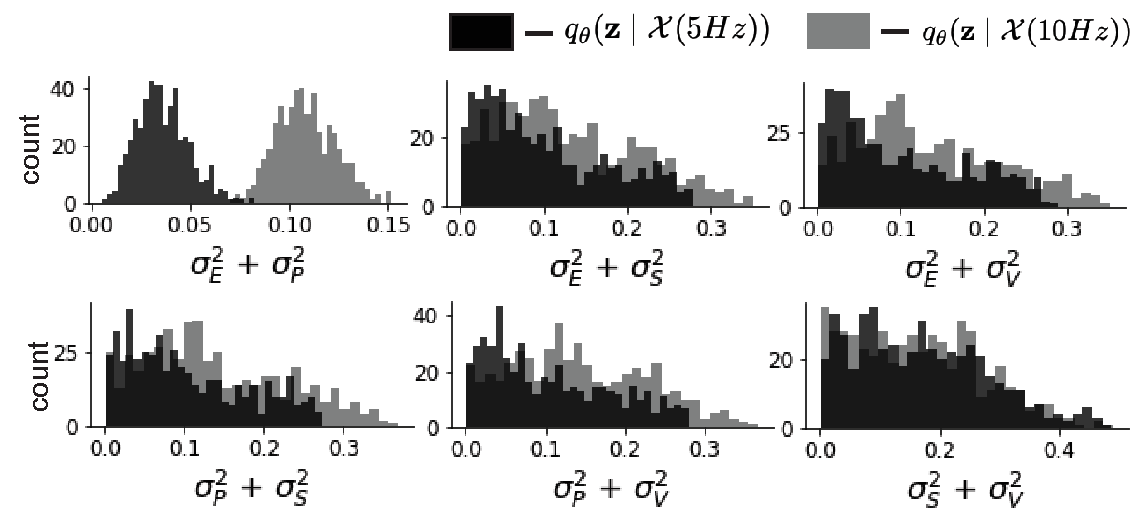
\includegraphics[scale=.8]{figures/figV1_2/figV1_2.pdf}
\end{center}
\end{figure}

\begin{equation}
W_{\text{fit}} =  \begin{bmatrix} W_{EE} & W_{EP} & W_{ES} & W_{EV} \\
W_{PE} & W_{PP} & W_{PS} & W_{PV} \\
W_{SE} & W_{SP} & W_{SS} & W_{SV} \\
W_{VE} & W_{VP} & W_{VS} & W_{VV}  \end{bmatrix} = 
 \begin{bmatrix} 2.18 & -1.19 & -.594 & -.229 \\
 1.66 & -.651 & -.680 & -.242 \\
 .895 & -5.22 \times 10^{-3} & -1.51 \times 10^{-4}   & -.761 \\
 3.34 &  -2.31 & -.254  & -2.52 \times 10^{-4} \\
 \end{bmatrix},
\end{equation} 

\begin{equation}
\mathbf{h}_{b,\text{fit}} =
 \begin{bmatrix} .416 \\ .429 \\ .491 \\ .486 \end{bmatrix} ,
\end{equation} 
and
\begin{equation} 
\mathbf{h}_{c,\text{fit}} = 
\begin{bmatrix} .359 \\ .403 \\ 0 \\ 0 \end{bmatrix}.
\end{equation} 

To obtain rates on a realistic scale (100-fold greater), we map these fitted parameters to an equivalence class

\begin{figure}[h]
\caption{\small (V1 3)
EPI inferred distribution for $\mathcal{X}(10\text{ Hz})$.
 }
 \label{fig:V1_3}
\begin{center}
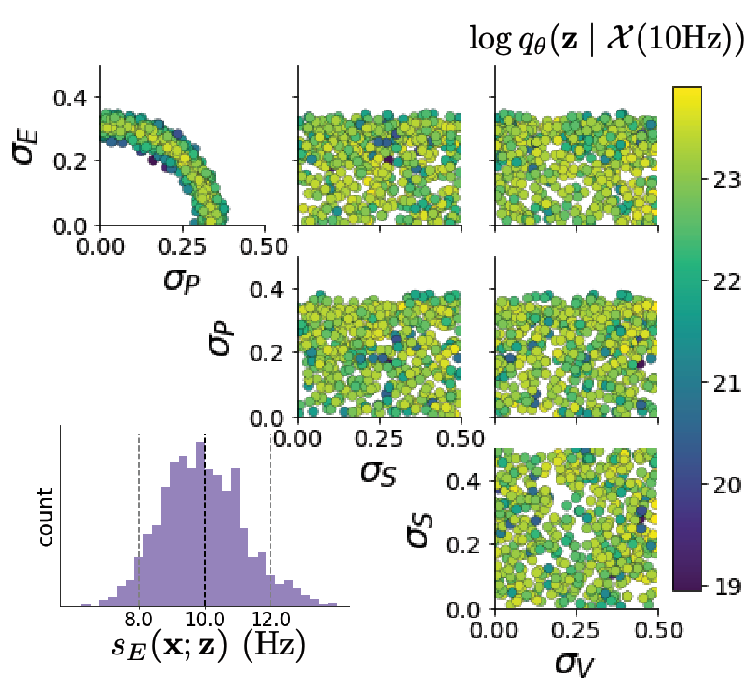
\includegraphics[scale=.8]{figures/figV1_3/figV1_3.pdf}
\end{center}
\end{figure}

\begin{equation}
W =  \begin{bmatrix} W_{EE} & W_{EP} & W_{ES} & W_{EV} \\
W_{PE} & W_{PP} & W_{PS} & W_{PV} \\
W_{SE} & W_{SP} & W_{SS} & W_{SV} \\
W_{VE} & W_{VP} & W_{VS} & W_{VV}  \end{bmatrix} = 
 \begin{bmatrix} .218 & -.119 & -.0594 & -.0229 \\
 .166 & -.0651 & -.068 & -.0242 \\
 .0895 & -5.22 \times 10^{-4} & -1.51 \times 10^{-5}   & -.0761 \\
 .334 &  -.231 & -.0254  & -2.52 \times 10^{-5} \\
 \end{bmatrix},
\end{equation} 

\begin{equation}
\mathbf{h}_b =  \begin{bmatrix} h_{b,E} \\ h_{b,P} \\ h_{b,S} \\ h_{b,V} \end{bmatrix} =
 \begin{bmatrix} 4.16 \\ 4.29 \\ 4.91 \\ 4.86 \end{bmatrix} ,
\end{equation} 
and
\begin{equation} 
\mathbf{h}_c = \begin{bmatrix} h_{c,E} \\ h_{c,P} \\ h_{c,S} \\ h_{c,V} \end{bmatrix} = 
\begin{bmatrix} 3.59 \\ 4.03 \\ 0 \\ 0 \end{bmatrix}.
\end{equation} 

Circuit responses are simulated using $T = 200$ time steps at $dt = 0.5\text{ms}$ from an initial condition drawn from $\mathbf{x}(0) \sim U\left[10\text{ Hz}, 25\text{ Hz}\right]$.
Standard deviation of the E-population $s_E(\mathbf{x}; \mathbf{z})$ is calculated as the square root of the temporal variance from $t_{ss} = 75\text{ms}$ to $Tdt = 100\text{ms}$ averaged over 100 independent trials.
\begin{equation}
s_E(\mathbf{x}; \mathbf{z}) =\mathbb{E}_{x}\left[\sqrt{\mathbb{E}_{t > t_{ss}}\left[\left(x_E(t) -\mathbb{E}_{t > t_{ss}}\left[ x_E(t) \right]\right)^2 \right]}\right]
\end{equation}

For EPI in Fig \ref{fig:V1}D-E, we used a real NVP architecture with three Real NVP coupling layers and two-layer neural networks of 50 units per layer.
The normalizing flow architecture mapped $z_0 \sim \mathcal{N}(\mathbf{0}, I)$ to a support of $\mathbf{z} = [\sigma_E, \sigma_P, \sigma_S, \sigma_V] \in [0.0, 0.5]^4$.
EPI optimization was run using three different random seeds for architecture initialization $\bm{\theta}$ with an augmented Lagrangian coefficient of $c_0 = 10^{-1}$, a batch size $n=100$, and $\beta = 2$.
The distributions shown are those of the architectures converging with criteria $N_{\text{test}} = 100$ at greatest entropy across random seeds.

In Fig. \ref{fig:V1}E, we visualize the modes of $q_{\bm{\theta}}(\mathbf{z} \mid \mathcal{X})$ throughout the $\sigma_E$-$\sigma_P$ marginal.
Specifically, we calculated
\begin{equation}
\begin{split}
\mathbf{z}^*(\sigma_{P,\text{fixed}}) = &\argmax_{\mathbf{z}} \log q_{\bm{\theta}}(\mathbf{z} \mid \mathcal{X}) \\
&\text{s.t. } \sigma_P = \sigma_{P,\text{fixed}}\
\end{split}
\end{equation}
At each mode $\mathbf{z}^*$, we calculated the Hessian and visualized the sensitivity dimension in the direction of positive $\sigma_E$.

\begin{figure}[h]
\caption{\small (V1 4)
Optimization for V1
 }
 \label{fig:V1_4}
\begin{center}
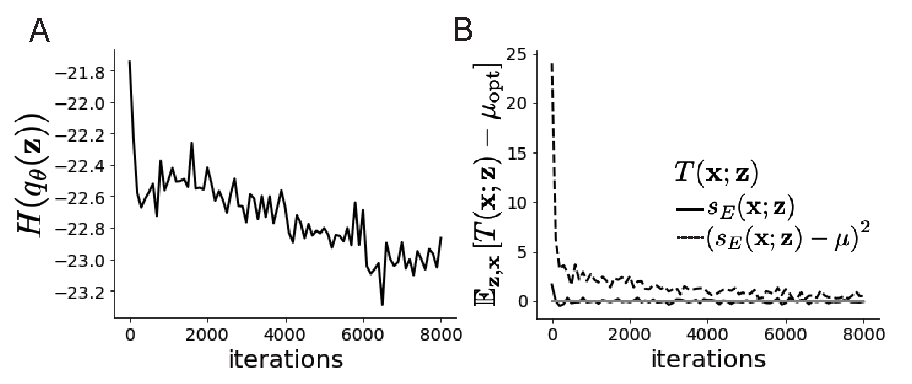
\includegraphics[scale=.8]{figures/figV1_4/figV1_4.pdf}
\end{center}
\end{figure}

\subsubsection{Primary visual cortex: challenges to analysis}\label{methods_V1_complexity}
TODO Agostina and I are putting this together now.

\subsubsection{Superior colliculus}\label{methods_SC}
The ability to switch between two separate tasks throughout randomly interleaved trials, or ``rapid task switching," has been studied in rats, and midbrain superior colliculus (SC) has been show to play an important in this computation \cite{duan2015requirement}.
Neural recordings in SC exhibited two populations of neurons that simultaneously represented both task context (Pro or Anti) and motor response (contralateral or ipsilateral to the recorded side), which led to the distinction of two functional classes: the Pro/Contra and Anti/Ipsi neurons \cite{duan2018collicular}.
Given this evidence, Duan et al. proposed a model with four functionally-defined neuron-type populations: two in each hemisphere corresponding to the Pro/Contra and Anti/Ipsi populations.  
We study how the connectivity of this neural circuit governs rapid task switching ability.

The four populations of this model are denoted as left Pro (LP), left Anti (LA), right Pro (RP) and right Anti (RA).  
Each unit has an activity ($x_\alpha$) and internal variable ($u_\alpha$) related by
\begin{equation}
x_\alpha = \phi(u_\alpha) = \left(\frac{1}{2}\tanh\left(\frac{u_\alpha - a}{b}\right)+ \frac{1}{2} \right),
\end{equation}
where $\alpha \in \{LP, LA, RA, RP\}$, $a = 0.05$ and $b = 0.5$ control the position and shape of the nonlinearity.
We order the neural populations of $x$ and $u$ in the following manner
\begin{equation}
\mathbf{x} = \begin{bmatrix} x_{LP} \\ x_{LA} \\ x_{RP} \\ x_{RA} \end{bmatrix} \hspace{2cm} \mathbf{u} = \begin{bmatrix} u_{LP} \\ u_{LA} \\ u_{RP} \\ u_{RA} \end{bmatrix},
\end{equation}
which evolve according to
\begin{equation}
\tau \frac{d\mathbf{u}}{dt} = -\mathbf{u} + W\mathbf{x} + \mathbf{h} + d\mathbf{B}.
\end{equation}
with time constant $\tau = 0.09s$, step size 24ms and Gaussian noise $d\mathbf{B}$ of variance $0.2^2$.
These hyperparameter values are motivated by modeling choices and results from \cite{duan2018collicular}.

\begin{figure}
\begin{center}
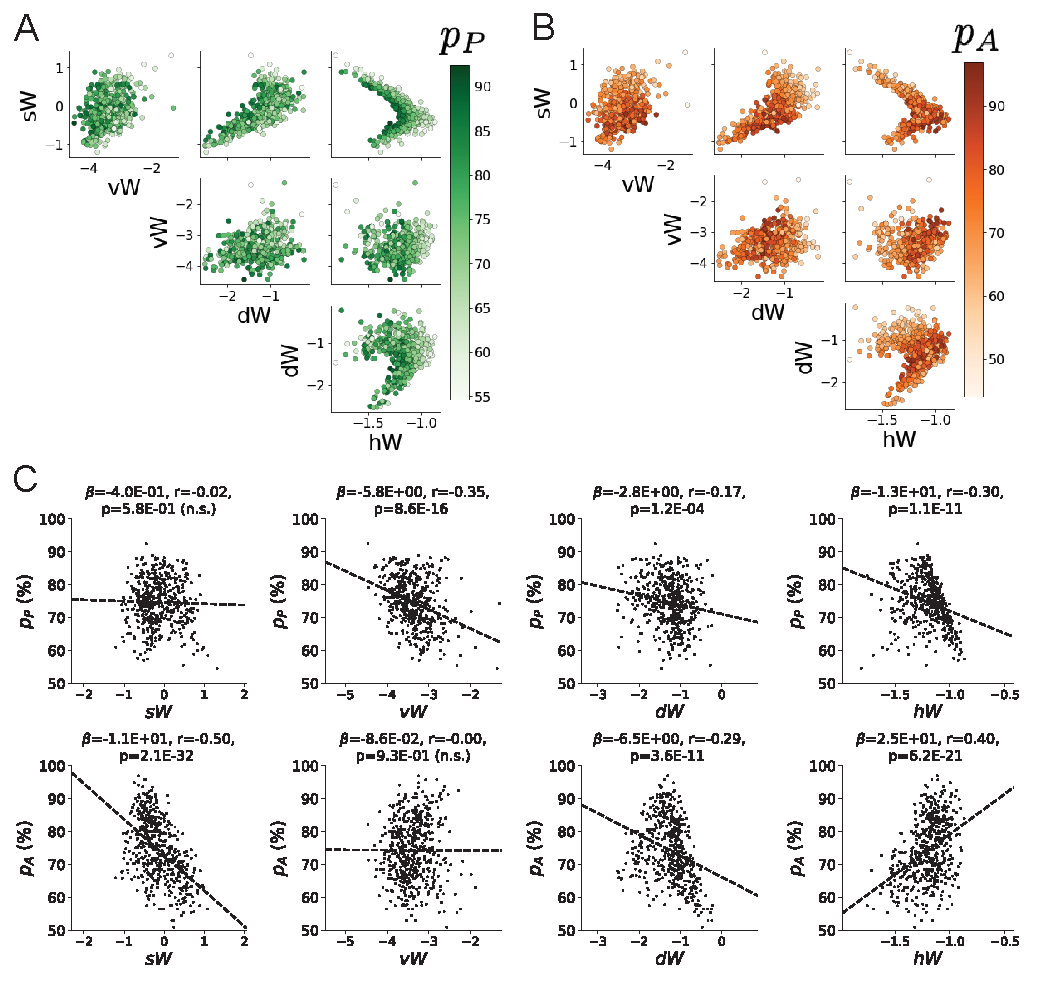
\includegraphics[scale=0.9]{figures/figSC1/figSC1.pdf}
\end{center}
\caption{\small (SC1): \textbf{A}. Same pairplot as Fig. \ref{fig:SC}C colored by Pro task accuracy.  
\textbf{B}. Same as A colored by Anti task accuracy.  
\textbf{C}. Connectivity parameters of EPI distributions versus task accuracies.  $\beta$ is slope coefficient of linear regression, $r$ is correlation, and $p$ is the two-tailed p-value.
}
\label{fig:SC1}
\end{figure}

\begin{figure}
\begin{center}
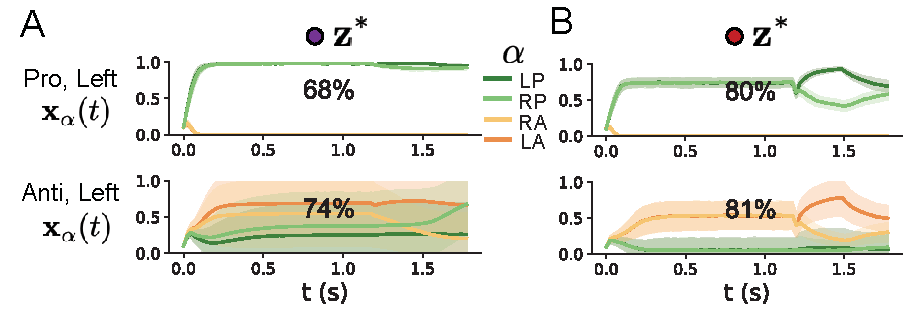
\includegraphics[scale=0.7]{figures/figSC2/figSC2.pdf}
\end{center}
\caption{\small (SC2):  
\textbf{A}. Simulations in network regime 1 ($hW_{\text{fixed}} = -1.2$) (center) with simulations given connectivity perturbations in the negative direction of the sensitivity vector $\mathbf{v}_1$ (left) and positive direction (right).
\textbf{B}. Same as A for network regime 2.
}
\label{fig:SC2}
\end{figure}

The weight matrix has 4 parameters for self $sW$, vertical $vW$, horizontal $hW$, and diagonal $dW$ connections:
\begin{equation}
W = \begin{bmatrix} sW & vW & hW & dW \\ vW & sW & dW  & hW \\ hW & dW & sW & vW \\ dW  & hW & vW  & sW \end{bmatrix}.
\end{equation}
We study the role of parameters $\mathbf{z} = [sW, vW, hW, dW]^\top$ in rapid task switching.

The circuit receives four different inputs throughout each trial, which has a total length of 1.8s.
\begin{equation}
\mathbf{h} = \mathbf{h}_{\text{constant}}  + \mathbf{h}_{\text{P,bias}} + \mathbf{h}_{\text{rule}} +  \mathbf{h}_{\text{choice-period}} + \mathbf{h}_{\text{light}}.
\end{equation}
There is a constant input to every population,
\begin{equation}\mathbf{h}_{\text{constant}} = I_{\text{constant}} [1, 1, 1, 1]\top,
\end{equation}
 a bias to the Pro populations
\begin{equation}\mathbf{h}_{\text{P,bias}} = I_{\text{P,bias}} [1, 0, 1, 0]\top,
\end{equation}
rule-based input depending on the condition
\begin{equation}\mathbf{h}_{\text{P,rule}}(t) = \begin{cases}
                           I_{\text{P,rule}} [1, 0, 1, 0]^\top,& \text{if } t\leq 1.2s \\
                            0,              & \text{otherwise}
                         \end{cases}
\end{equation}
\begin{equation} \mathbf{h}_{\text{A,rule}}(t) = \begin{cases}
                           I_{\text{A,rule}} [0, 1, 0, 1]^\top,& \text{if } t\leq 1.2s \\
                            0,              & \text{otherwise}
                         \end{cases},
\end{equation}
a choice-period input
\begin{equation} \mathbf{h}_{\text{choice}}(t) = \begin{cases}
                           I_{\text{choice}} [1, 1, 1, 1]^\top,& \text{if } t > 1.2s \\
                            0,              & \text{otherwise}
                         \end{cases},
\end{equation}
and an input to the right or left-side depending on where the light stimulus is delivered    
\begin{equation}  \mathbf{h}_{\text{light}}(t) = \begin{cases}
                           I_{\text{light}} [1, 1, 0, 0]^\top,& \text{if } 1.2s < t < 1.5s \text{ and Left} \\
                           I_{\text{light}} [0, 0, 1, 1]^\top,& \text{if } 1.2s < t < 1.5s \text{ and Right} \\
                            0,              & \text{otherwise}
                         \end{cases}.
\end{equation}
The input parameterization was fixed to $I_{\text{constant}} = 0.75$, $I_{\text{P,bias}} = 0.5 $, $I_{\text{P,rule}} = 0.6$,  $I_{\text{A,rule}} = 0.6$,  $I_{\text{choice}} = 0.25$,  and $I_{\text{light}} = 0.5$.


\begin{figure}
\begin{center}
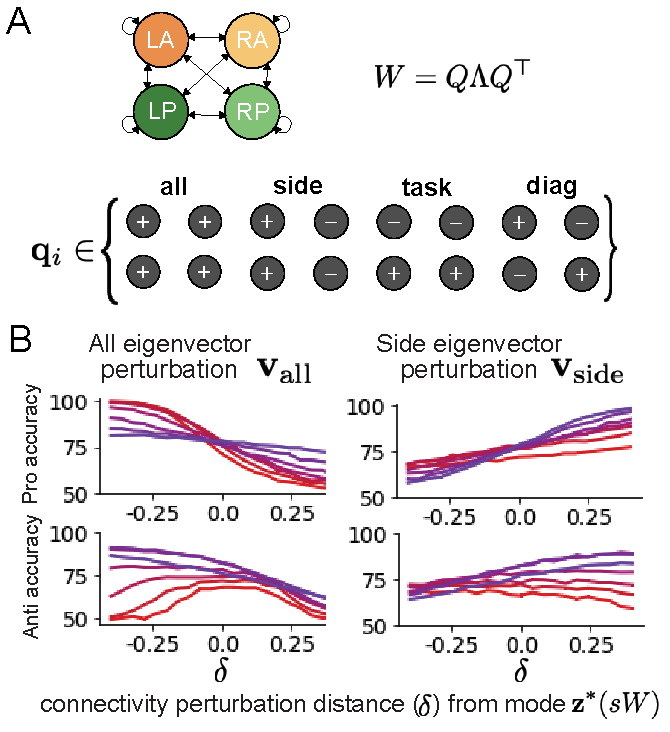
\includegraphics[scale=0.9]{figures/figSC3/figSC3.pdf}
\end{center}
\caption{\small (SC3):  
\textbf{A}. Invariant eigenvectors of connectivity matrix $W$.
\textbf{B}. Accuracies for connectivity perturbations for increasing $\lambda_{\text{all}}$ and $\lambda_{\text{side}}$ (rest shown in Fig. \ref{fig:SC}D).
}
\label{fig:SC3}
\end{figure}

The accuracies of each task $p_P$ and $p_A$ are calculated as
\begin{equation}
p_P(\mathbf{x}; \mathbf{z}) = \mathbb{E}_{\mathbf{x}}\left[\Theta[x_{LP}(t=1.8s) - x_{RP}(t=1.8s)]\right]
\end{equation}
and 
\begin{equation}
p_A(\mathbf{x}; \mathbf{z}) = \mathbb{E}_{\mathbf{x}}\left[\Theta[x_{RP}(t=1.8s) - x_{LP}(t=1.8s)]\right]
\end{equation}
given that the stimulus is on the left side, where $\Theta$ is the Heaviside step function, and the accuracy is averaged over 200 independent trials.  The Heaviside step function is approximated as
\begin{equation}
\Theta(\mathbf{x}) = \text{sigmoid}(\beta \mathbf{x}),
\end{equation}
where $\beta = 100$.

\begin{figure}
\begin{center}
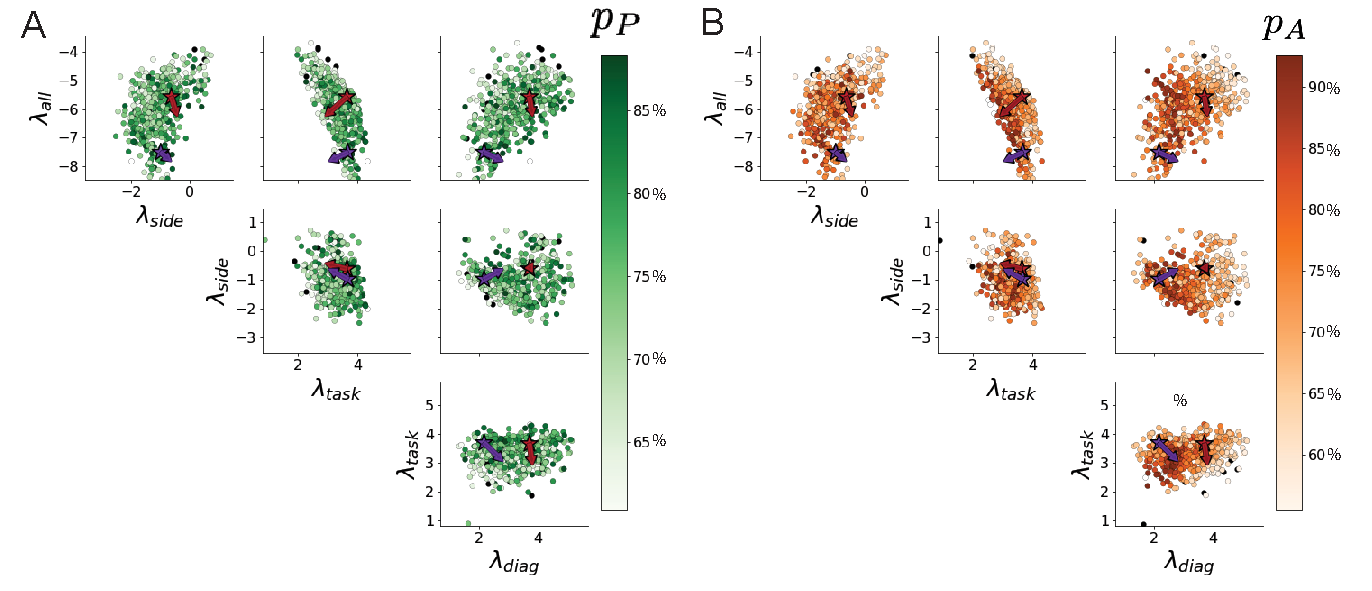
\includegraphics[scale=0.8]{figures/figSC4/figSC4.pdf}
\end{center}
\caption{\small (SC4):  \textbf{A}. The individual parameters of each mode throughout the two regimes.
\textbf{B}. The individual sensitivities of parameters of each mode throughout the two regimes.
}
\label{fig:SC4}
\end{figure}

\begin{figure}
\begin{center}
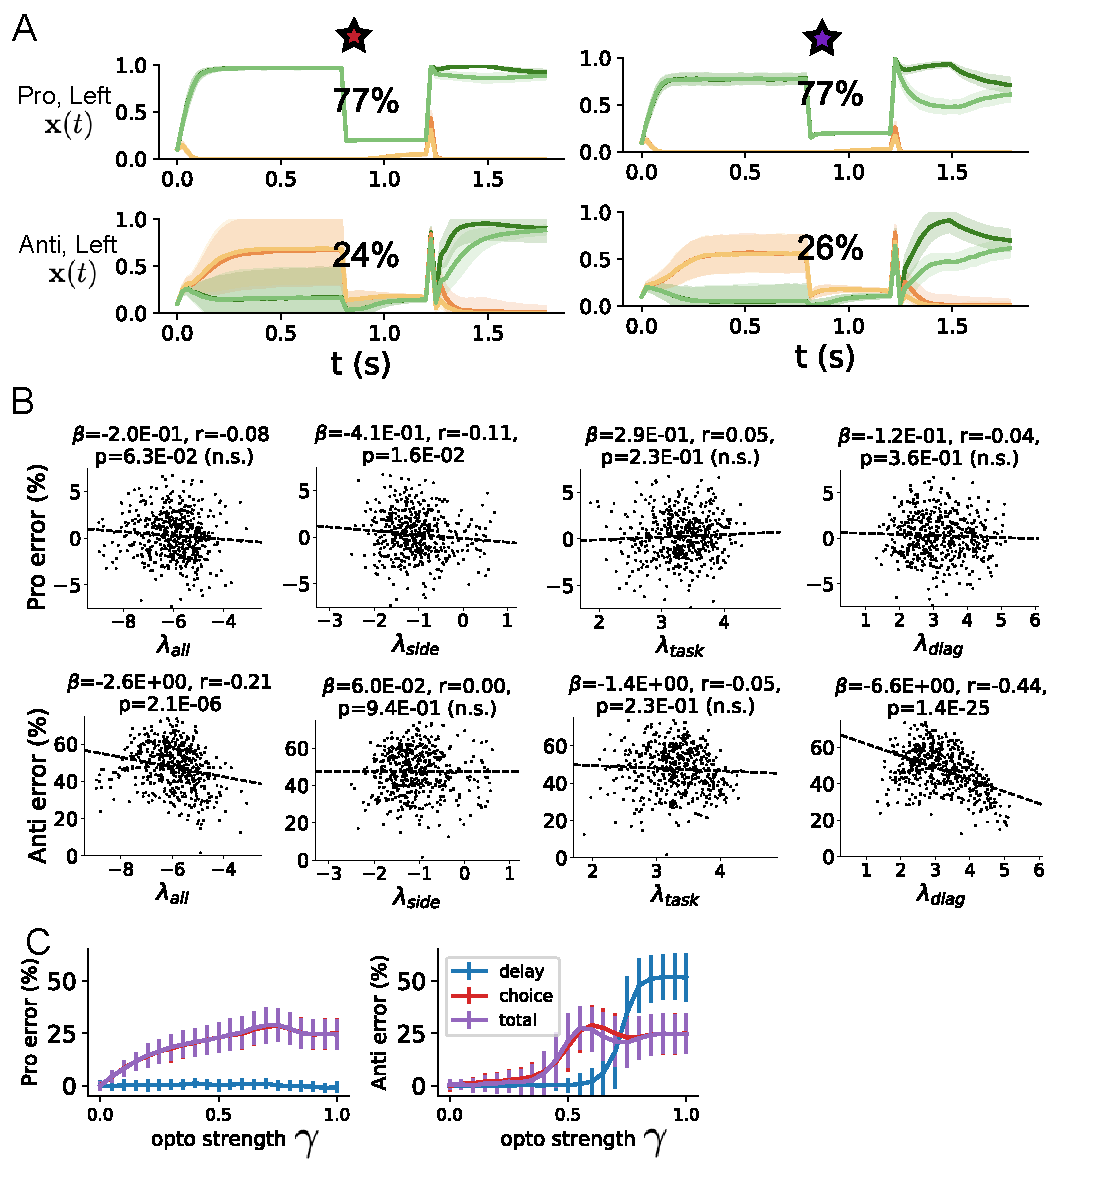
\includegraphics[scale=0.8]{figures/figSC5/figSC5.pdf}
\end{center}
\caption{\small (SC5): 
\textbf{A}. Response of each parameter regime to optogenetic silencing during the delay period.
\textbf{B}. Error induced by delay period inactivation with increasing optogenetic strength.  Means and standard deviations are calculated across the entire EPI distribution.
}
\label{fig:SC5}
\end{figure}

Writing the EPI distribution as a maximum entropy distribution, $T(\mathbf{x}, \mathbf{z})$ is comprised of both these first and second moments of the accuracy in each task (as in Equations \ref{eq:moments} and \ref{eq:mu_opt})
\begin{equation} 
T(\mathbf{x}; \mathbf{z}) = \begin{bmatrix} p_P(\mathbf{x}; \mathbf{z}) \\ p_A(\mathbf{x}; \mathbf{z}) \\ \left(p_P(\mathbf{x}; \mathbf{z}) - 75\% \right)^2 \\ \left(p_A(\mathbf{x}; \mathbf{z}) - 75\% \right)^2 \end{bmatrix},
\end{equation}
\begin{equation} 
\bm{\mu}_{\text{opt}} = \begin{bmatrix} 75\% \\ 75\% \\ 7.5\%^2 \\ 7.5\%^2 \end{bmatrix}.
\end{equation}
Throughout optimization, the augmented Lagrangian parameters $\eta$ and $c$, were updated after each epoch of 2,000 iterations (see Section \ref{methods_AL_opt}).  
The optimization converged after ten epochs (Fig. \ref{fig:SC6}).


\begin{figure}
\begin{center}
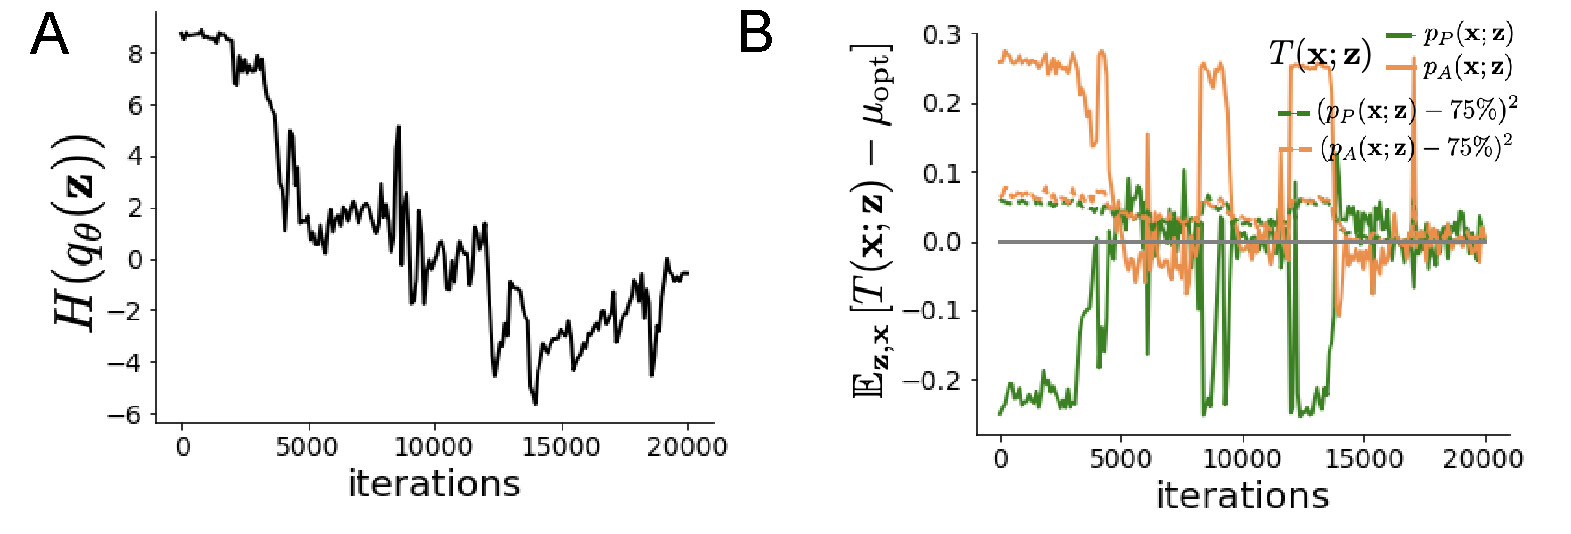
\includegraphics[scale=0.5]{figures/figSC6/figSC6.pdf}
\end{center}
\caption{\small (SC6): 
\textbf{A}. Entropy throughout optimization. 
\textbf{B}. The emergent property statistic means and variances converge to their constraints at 20,000 iterations following the tenth augmented Lagrangian epoch.
}
\label{fig:SC6}
\end{figure}

For EPI in Fig. \ref{fig:SC}C, we used a real NVP architecture with three coupling layers of affine transformations parameterized by two-layer neural networks of 50 units per layer.
The initial distribution was a standard isotropic gaussian $z_0 \sim \mathcal{N}(\mathbf{0}, I)$ mapped to a support of $\mathbf{z}_i \in [-5, 5]$. 
We used an augmented Lagrangian coefficient of $c_0 = 10^{2}$, a batch size $n=100$, and $\beta=2$.
The distribution converged with criteria $N_{\text{test}} = 25$.

The EPI distribution of SC model connectivities producing rapid task switching has interesting structure.
Throughout $q_{\bm{theta}}(\mathbf{z} \mid \mathcal{X})$, we see that the probability distribution is narrow in $hW$ (Fig. \ref{fig:SC}C).
This suggests that rapid task switching is sensitive to changes in $hW$, but this is only a single parameter.
The local structure of the distribution varies across parameter space, and thus the nature in which parameter combinations affect rapid task switching.
From visual inspection, we may hypothesize that there are two distinct regimes, most easily visualized in the $sW$-$hW$ marginal distribution: one where $sW$ and $hW$ are correlated for greater $sW$ and one where $sW$ and $hW$ are anticorrelated for lesser $sW$.

We sought two sets of parameters in this distribution representative of each regime, so that we could assess their implications on computation.
For fixed values of $hW$, we hypothesized that there are two modes: one in each regime of greater and lesser $sW$.
To begin, we found one mode for each regime at $hW_{\text{fixed}} = -1.5$ using 200 steps of gradient ascent of the deep probability distribution $q_{\bm{\theta}}(\mathbf{z} \mid \mathcal{X})$.
In regime 1, the initialization had positive $sW$, and the initialization had negative $sW$ in regime 2, which led to disparate modes (Fig. \ref{fig:SC4} top).
These modes were then used as the initialization to find the next mode at $hW_{\text{fixed}} = -1.4$ and so on.
200 steps of gradient ascent were always taken, and learning rates of $2.5 \times 10^-4$ and $5 \times 10^-4$ were used for regimes 1 and 2, respectively.
Each of these modes is denoted $\mathbf{z}^*(hW_{\text{fixed}}, r)$ for regime $r \in \{1, 2\}$.

At each mode, we measure the sensitivity dimension (that of most negative eigenvalue in the Hessian of the EPI distribution) $\mathbf{v}_1(\mathbf{z}^*)$.
To resolve sign degeneracy in eigenvectors, we chose $\mathbf{v}_1(\mathbf{z}^*)$ to have negative element in $hW$.
This tells us what parameter combination rapid task switching is most sensitive to at this parameter choice in the regime.
We see that while the modes of each regime gradually converge to similar connectivities at $hW_{\text{fixed}} = -1.05$ (Fig. \ref{fig:SC4} top), the sensitivity dimensions remain categorically different throughout the two regimes (Fig. \ref{fig:SC4} bottom)
Only at $hW_{\text{fixed}} = -1.05$ is there a flip in sensitivity from regime 2 to regime 1 (in $\mathbf{v}_1(\mathbf{z}^*)_{sW}$ and $\mathbf{v}_1(\mathbf{z}^*)_{hW}$).
There is thus some ambiguity regarding the ``regime" of $\mathbf{z}^*(-1.05, 2)$, since the mode is derived from an initialization in regime 2, but has sensitivity like regime 1.
We can consider this as an intermediate transitionary region of parameter space between the two regimes.
To emphasize this, $\mathbf{z}^*(-1.05, 1)$ and $\mathbf{z}^*(-1.05, 2)$ have the same color.

To understand the connectivity mechanisms governing task accuracy, we took the eigendecomposition of the symmetric connectivity matrices $W = Q\Lambda Q^{-1}$, which results in the same basis vectors $\mathbf{q}_i$ for all $W$ parameterized by $\mathbf{z}$ (Fig. \ref{fig:SC3}A). 
These basis vectors have intuitive roles in processing for this task, and are accordingly named the \textit{all} eigenmode - all neurons co-fluctuate, \textit{side} eigenmode - one side dominates the other, \textit{task} eigenmode - the Pro or Anti populations dominate the other, and \textit{diag} mode - Pro- and Anti-populations of opposite hemispheres dominate the opposite pair. 
Due to the parametric structure of the connectivity matrix, the parameters $\mathbf{z}$ are a linear function of the eigenvalues $\bm{\lambda} = [\lambda_{\text{all}}, \lambda_{\text{side}}, \lambda_{\text{task}}\lambda_{\text{diag}}]^\top$ associated with these eigenmodes.
\begin{equation}
\mathbf{z} = A\bm{\lambda}
\end{equation}
\begin{equation}
A = \frac{1}{4} \begin{bmatrix} 1 & 1 & 1 & 1 \\ 1 & -1 & -1 & 1 \\ 1 & 1 & -1 & -1 \\ 1 & -1 & 1 & -1 \end{bmatrix}.
\end{equation}

We are interested in the effect of raising or lowering the amplification of each eigenmode in the connectivity matrix.
To test this, we calculate the unit vector of changes in the connectivity $\mathbf{z}$ that result from a change in the associated eigenvalues
\begin{equation}
\mathbf{v}_{\text{a}} = \frac{\frac{\partial \mathbf{z}}{\partial \lambda_{\text{a}}}}{|\frac{\partial \mathbf{z}}{\partial \lambda_{\text{a}}}|_2},
\end{equation}
where
\begin{equation} \label{eq:dzdlambda}
\frac{\partial \mathbf{z}}{\partial \lambda_{\text{a}}} = A\mathbf{e}_{\text{a}},
\end{equation}
and e.g. $\mathbf{e}_{\text{all}} = [1, 0, 0, 0]^\top$.
So $\mathbf{v}_{\text{a}}$ is the normalized column of A corresponding to eigenmode $a$.
While perturbations in the sensitivity dimension $\mathbf{v}_1(\mathbf{z}^*)$ adapt with the mode $\mathbf{z}^*$ chosen, perturbations in $\mathbf{v}_a$ for $a \in \{\text{all}, \text{side}, \text{text}, \text{diag}\}$ are invariant to $\mathbf{z}$ (Equation \ref{eq:dzdlambda}).

To understand the connectivity mechanisms that distinguish these two regimes, we perturb connectivity at each mode in dimensions that have well defined roles in processing for the Pro and Anti tasks.
A convenient property of this connectivity parameterization is that there are $\mathbf{z}$-invariant eigenmodes of connectivity, whose eigenvalues (or degree of amplification) change with $\mathbf{z}$.
These eigenmodes have intuitive roles in processing in each task, and are accordingly named the \textit{all}, \textit{side}, \textit{task}, and \textit{diag} eigenmodes (see Section \ref{methods_SC}).
Furthermore, the parameter dimension $\mathbf{v}_a$ ($a \in \{\text{all}, \text{side}, \text{task}, \text{ and diag}\}$) that increases the eigenvalue of connectivity $\lambda_a$ is $\mathbf{z}$-invariant (unlike the sensitivity dimension $\mathbf{v}_1(\mathbf{z})$) and $\mathbf{v}_a \perp \mathbf{v}_{b \neq a}$.
Thus, by changing the degree of amplification of each processing mode by  perturbing $\mathbf{z}$ along $\mathbf{v}_a$, we can elicit the differentiating properties of the two regimes.

Through these connectivity perturbation analyses, we found that increasing $\lambda_{\text{task}}$ strongly reduced Pro accuracy in regime 1, yet strongly reduced Anti accuracy in regime 2.
This suggests that stronger task representations can inhibit both Pro and Anti task performance in different contexts.
Furthermore, changing $\lambda_{\text{task}}$ in either direction decreases Anti performance in regime 1, showing that Anti task performance in regime 1 is dependent on a specific level of task representation.
We also found that with increasing $\lambda_{\text{diag}}$, Pro accuracy increased in both regimes, but there were opposite effects on Anti accuracy.
In regime 1, stronger amplification of diagonal population patterns decreased Anti accuracy, while in regime 2 accuracy increased.
These findings give us an understanding of the mechanistic differences in computation enabling rapid task switching in each regime.


%
%These eigenvalue changes are evident in the simulations of connectivity perturbations away from the modes (Fig. \ref{fig:SC2}).
%As the component of connectivity along $\mathbf{v}_1$ and $\mathbf{v}_2$ becomes stronger (left-to-right), there is less separation between Pro an Anti populations (lower $\lambda_{\text{task}}$) and greater separation between Left and Right populations following stimulus presentation (greater $\lambda_{\text{side}}$).
%A key differentiating factor is that $\mathbf{v}_1$ substantially increases $\lambda_{\text{diag}}$, while $\mathbf{v}_2$ does not.

We tested whether the inferred SC model connectivities could reproduce experimental effects of optogenetic inactivation in rats \cite{duan2015requirement}.
During periods of simulated optogenetic inactivation, activity was decreased proportional to the optogenetic strength $\gamma$
\begin{equation}
x_\alpha = (1-\gamma)\phi(u_\alpha).
\end{equation}
Delay period inactivation was from $0.8 < t < 1.2$, choice period inactivation was for $t > 1.2$ and total inactivation was for the entire trial.

\end{document}

